%!TEX root = ../thesis.tex

\chapter{Application of tipping point techniques to tropical cyclones}
\label{chap:cyclones}
\graphicspath{{Chap_Cyclones/Figs/}} % Define Graphics Path 
% References in this chapter have the identifier "TC"
% for Tropical Cyclones

In this chapter, we apply the techniques described previously to the real geophysical problem of providing an early warning signal for the approach of a moving tropical cyclone\footnote{A tropical cyclone is referred to as a ‘hurricane' when it occurs in the Atlantic Ocean and north-eastern Pacific Ocean  and a ‘typhoon' when in the north-western Pacific Ocean. In the south Pacific or Indian Ocean, comparable storms are referred to simply as ‘tropical cyclones' or ‘cyclones' \citep{NOAA_cyclones}. These naming conventions are not always abided by (e.g. Australian ‘hurricanes') and do not denote any differences in the physical properties of the storms other than geographic location.}. Typically, a steep drop in sea-level pressure is observed at the arrival of a cyclone, as shown in figure~\ref{fig:TC:SLP14}. {\Red{ This sudden, or `abrupt', change in the state of the system is not bifurcational in the sense that there are multiple stable system states, but it is nonetheless a tipping event in the general sense as defined by \cite{kuehn2011mathematical}, and we note that non-bifurcational tipping points (e.g. rate-induced tipping, noise-induced tipping, etc.) have previously been analysed using techniques similar to the ones used in this thesis \citep{livina2011,ashwin2012}. Similarly, there is a steep rise in wind speed at the same time (the same tipping point) and the early warning indicators we have developed may also be applied to the  wind speed time series beside the sea-level pressure.

The hypothesis is that it is possible to detect or predict this observed tipping point (the abrupt change in pressure and wind speed) using the same methods previously used to analyse examples of noise-induced, transitional or bifurcational tipping points. }}

A large tropical cyclone may extend hundreds of kilometres from its centre and a location on the future trajectory of such a storm experiences high winds several hours or days before the arrival of 200km/h winds. We expect, therefore, that the study of the weather variable at a fixed location will provide an early warning signal for the arrival of a tropical cyclone. The rise in wind speed itself acts as such a signal in a short (12 hour) period, but we are interested in the possibility that the tipping point techniques described in chapters~\ref{chap:1D} and~\ref{chap:2D} will provide an early warning signal when applied in this context.

{\Red{ We have no specific reason to expect that these EWS methods will be effective in this particular application but, in general, the sudden qualitative change in the system and the fact the a cyclone can be felt some way off make this a good candidate for investigation and experimentation.}}

In section~\ref{sec:TC:data} we give a description of the data used throughout this chapter, which has been obtained from the NOAA HURDAT2 database  \citep{HURDAT2} and the Met Office HadISD database \citep{HadISD}. In section~\ref{sec:TC:1Dtechniques} we apply the ACF1, DFA and PS indicators (see chapter~\ref{chap:1D}) to the sea-level pressure time series data from locations on the paths of fourteen tropical cyclones. In section~\ref{sec:TC:2Dtechniques} the same fourteen {\Red data sets} are used but both the sea-level pressure and the wind speed variables are considered and the techniques described in chapter~\ref{chap:2D} are applied to the two variables.

In section~\ref{sec:TC:field_data} we use sea-level pressure time series from several locations in a region through which a tropical cyclone passes. We apply the techniques introduced in section~\ref{sec:2D:ExtensionToGridded} to visualise the rise of a tipping point indicator over the area as the tropical cyclone approaches. This idea is further developed in section~\ref{sec:TC:Model} {\Red{where a model of the approaching cyclone is parametrised using the observed values of the tipping point indicators. The model is developed in order to verify the use of these indicators in the study of the tropical cyclone system.}}

\section{Description of data}
\label{sec:TC:data}

\subsection{The HURDAT2 database}
\label{subsec:TC:data:HURDAT}

During this study it was necessary to have track data of several Atlantic hurricanes, this was obtained from the NOAA national hurricane centre's HURDAT2 database \citep{landsea2013, HURDAT2}. This dataset is presented as a comma-delimited, text format with six-hourly information on the location, maximum winds, central pressure, and size of all known tropical cyclones and subtropical cyclones. We have only used the location data (given as latitude-longitude coordinates) and have not performed any additional processing of this data.


\subsection{The HadISD database}
\label{subsec:TC:data:HadISD}

For the purposes of our study we use sea-level pressure (SLP) and wind speed data from weather stations. These data are obtained from the HadISD 2017 data set \citep{HadISD_smith,HadISD_dunn12,HadISD_dunn14,HadISD_dunn16,HadISD} maintained by, and available from, the UK Met Office. The sea-level pressure and wind speed data provided by HadISD are raw data given at one-hour intervals, the Met Office applies a filter so that weather stations which provide very sparse data are disregarded \citep{HadISD_dunn12}, no other processing is applied.

The weather stations used in this study are selected for proximity to the landfall locations of tropical cyclones, and data are considered in a fifteen-day (360 hour) period before the time when the cyclone passes closest to the station. However, some of the weather stations provide very sparse data even after the Met Office's filtering, this is common at times when a tropical cyclone passes close to a station (presumably due to infrastructural damage). If fewer than 80\% of the time points have associated data, the time series is disregarded. Otherwise the data are interpolated linearly onto the entire hourly time series. We notice that weather stations on the United States mainland are more numerous than in other regions affected by tropical cyclones and also provide more consistent data. The examples used in this chapter are therefore dominated by Atlantic hurricanes making landfall in the USA.

In sections~\ref{sec:TC:1Dtechniques} and~\ref{sec:TC:2Dtechniques} we consider a single weather station associated with each cyclone, as close as possible to the landfall location, and we look at the single sea-level pressure and wind speed time series given at these stations. We consider 14 tropical cyclones selected for proximity of a weather station to the landfall location with reasonable data. Most of the cyclones selected, with the exceptions of Hurricane Jeanne and Hurricane Ernesto, are ranked category 4 or 5, using the SSHWS\footnote{The Saffir-Simpson hurricane wind scale (SSHWS) ranks cyclones based only on maximum one-minute sustained wind speeds. A cyclone with a wind speed of 209km/h or more is Category 4, with 251km/h or over is Category 5 \citep{NOAA_saffir}.}, at the time of landfall. These exceptions were included to broaden the scope of the study and because, although with a lower maximum wind speed, they exhibit a pronounced drop in pressure similar to the stronger cyclones. All 14 tropical cyclones are listed in table~\ref{tab:TC:14cyclones}, and the sea-level pressure time series are shown in figure~\ref{fig:TC:SLP14}. Many more than these 14 were considered initially, but in many cases a HadISD weather station did not exist close to the landfall location or, when it did, the data were sparse. 


\begin{table}
	\centering
	\begin{tabular}{ l  c  l  c  c  c }
		\hline
		\multirow{2}{*}{Name} & \multirow{2}{*}{Year} & \multirow{2}{*}{Location} & Min pressure & Max speed & Osc. amp. \\
		& & & (hPa) & (km/h) & (hPa) \\ 
		\hline \hline
		Flo     &  1990 & Shionomisaki (Japan)  & 890 & 270  & 0.91\\
		
		Andrew  &  1992 & Florida Keys (USA) & 922 & 280 & 1.09  \\

		Opal    &  1995 & Pensacola (USA) & 916 & 240 & 1.22\\
		
		Zeb	    &  1998 & Tuguegarao (Philippines)  & 900 & 285 & 1.15\\

		Floyd   &  1999 & Florida Keys (USA) & 921 & 250 & 1.15\\
		
		Charley &  2004 & Fort Myers (USA) & 941 & 240 & 1.17 \\
		
		Frances &  2004 & Florida Keys (USA) & 935 & 230 & 1.15 \\
		
		Jeanne  &  2004 & Florida Keys (USA) & 950 & 195 & 1.21 \\
		
		Katrina &  2005 & New Orleans (USA) & 902 & 280 & 1.24   \\
		
		Rita    &  2005 & Lake Charles (USA)  & 895 & 285 & 1.29  \\
		
		Ivan    &  2006 & Mobile (USA) & 910 & 270 & 1.18\\
		
		Ernesto &  2006 & Florida Keys (USA)  & 985 & 120 & 1.05\\
				
		Megi    &  2010 & Tuguegarao (Philippines) & 885 & 295 & 1.31  \\
		
		Hudhud  &  2014 & Vishakhapatnam (India)   & 950 & 260 & 1.29   \\
		\hline
	\end{tabular}
	\caption{The dates and locations of each of the 14 tropical cyclones considered. The "Location" column data is the identifying location recorded on the HadISD database for the weather station used in this study. The "Max speed" column gives the highest one-minute sustained wind speed (a value over 209~km/h puts the cyclone into SSHWS category 4 or higher). The data in the pressure and wind speed columns is not used in this study and is given for information only. It is obtained from the NOAA archive \citep{NOAA_archive} in the cases of the Atlantic hurricanes (those in the USA), and from \protect\url{www.wikipedia.org} otherwise. The column "Osc. amp." gives the amplitudes of the 12-hourly oscillations in the sea level pressure data from that weather station but in a period 50 to 15 days before the cyclone event (this is discussed in section~\ref{subsec:TC:data:oscillations}).}
	\label{tab:TC:14cyclones}
\end{table}

\begin{figure}
\centering
	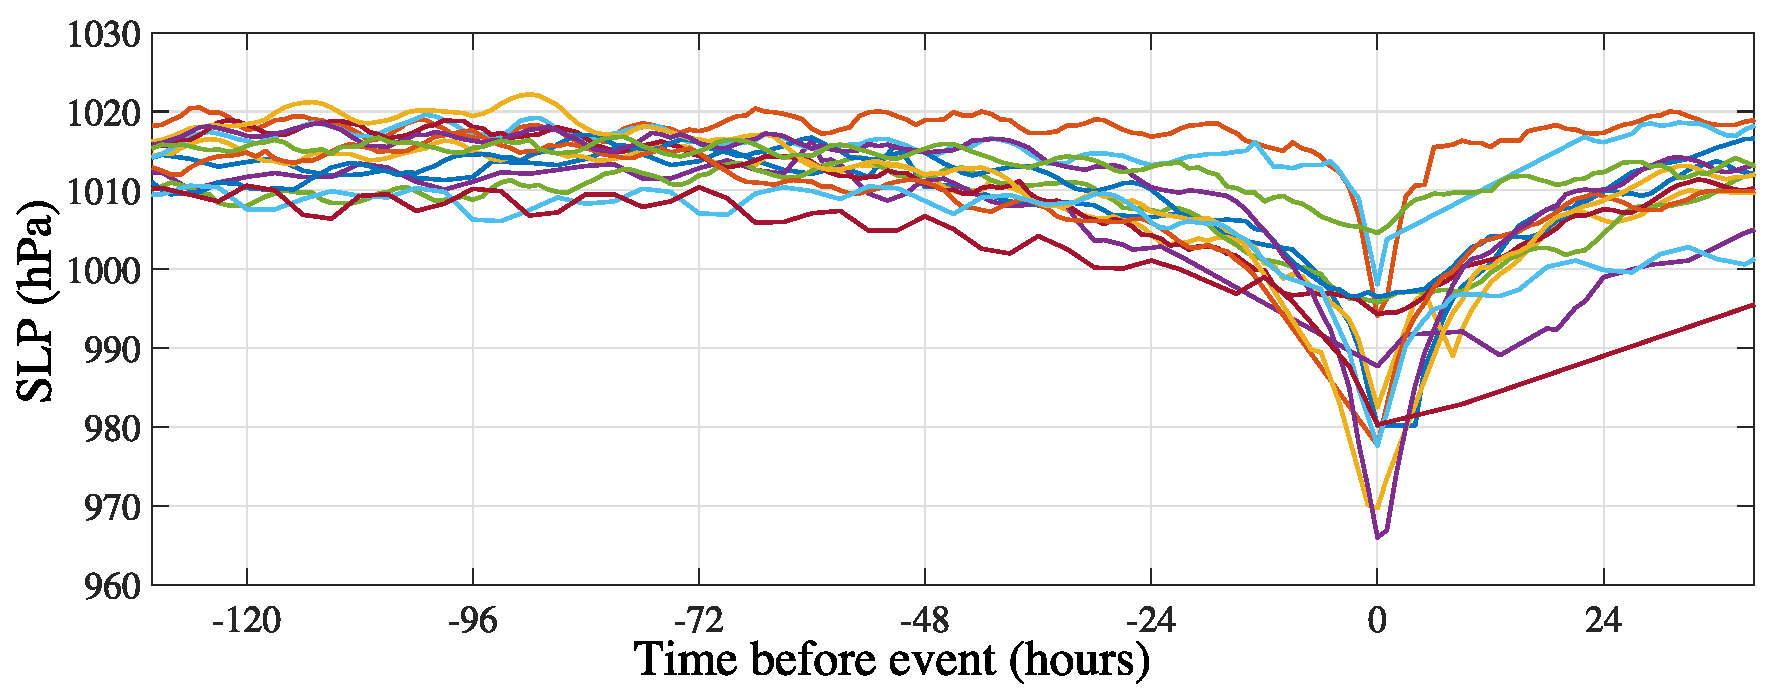
\includegraphics[width = 0.9\textwidth]{PlotSLP14}
	\caption{Sea-level pressure time series for the fourteen tropical cyclones selected in table~\ref{tab:TC:14cyclones}. The minimum point in the data is presumed to be the point closest to the time at which the cyclone was closest to the station and is set as time zero.
		\label{fig:TC:SLP14}}
\end{figure}

In section~\ref{sec:TC:field_data} we consider the data given by several weather stations in a region surrounding the path of the cyclone. Because of better availability of data, all the cyclones in this case are Atlantic hurricanes making landfall on the Caribbean or Florida coastlines of the United States. The eight hurricanes considered are listed in table \ref{tab:TC:9hurricanes}, Hurricane Andrew appears twice (labelled Andrew 1 and Andrew 2) because it made landfall twice: over Florida and then, two days later, over Louisiana. We therefore have a total of nine hurricanes. Again, we use the HadISD 2017 data set \citep{HadISD_dunn12,HadISD_dunn14,HadISD_dunn16,HadISD_smith}. {\Red{We take data from stations within 200~km of the landfall of each hurricane and a region is formed by the minimal rectangle containing all of the weather stations used, which amounts to $65$ stations at separate locations. In some cases the stations did not provide `good' time series data and so the number used in the analysis of each hurricane is lower than $65$ in each case and is between $21$ and $48$ stations depending on the hurricane (see column ``\# stations'' in table~\ref{tab:TC:9hurricanes})}}. We use the HURDAT2 track data \citep{landsea2013} (see section~\ref{subsec:TC:data:HURDAT}) in each case to find the point at which the hurricane entered this region. 

\begin{table}
	\centering
	\begin{tabular}{ l  l  l  c c }
		\hline
		Name & Date & Region & Entry point & \# stations\\
		\hline \hline
		Andrew 1 &  24 August 1992 &      Florida     &   [25.4N,    -79.0E] &21\\

		Andrew 2 &  26 August 1992 &      Louisiana  &  [29.8N,  -91.6E]&34\\

		Katrina &   29 August 2005 &     Louisiana &   [29.3N,   -89.6E]&45\\

		Wilma &     24 October 2005 &   Florida     &   [25.3N,    -82.7E]&34\\

		Gustav &  1 September 2008 &   Louisiana & [29.3N,    -90.8E]&46\\

		Matthew &  7 October 2016 & Florida     & [26.7N,    -79.0E]&32\\

		Harvey  &  25 August 2017 &      Texas       &  [25.2N,    -94.6E]&29\\

		Irma &        10 September 2017 & Florida    &  [24.5N,    -81.5E]&34\\

		Nate &       8 October 2017 &    Louisiana &   [29.3N,   -89.2E]&48\\
		\hline
	\end{tabular}
	\caption{\Red{ The dates and locations of each of the nine hurricanes selected. The entry point column gives the coordinates at which each hurricane entered the region, calculated using the HURDAT2 track data. Hurricane Andrew appears twice (labeled Andrew 1 and Andrew 2) because it made landfall twice: over Florida and then, two days later, over Louisiana. The column `\# stations' gives the number of weather stations in the region from which data was used when analysing each hurricane. }}\label{tab:TC:9hurricanes}
	% for i = 1:9
	% disp([SuperStruct(i).name,': ',num2str(size(SuperStruct(i).allValues,1))])
	% end
\end{table}

\subsection{Filtering sea-level pressure oscillations}
\label{subsec:TC:data:oscillations}

Upon inspection of the sea-level pressure data we see that there is a small, regular oscillation superimposed on the longer term fluctuations, figure~\ref{fig:TC:osc_and_powerspectrum}a shows this phenomenon at the Florida Keys station prior to Hurricane Andrew. An inspection of the power spectrum shows that the oscillations have a period of 12 hours (see figure~\ref{fig:TC:osc_and_powerspectrum}b) and are due to the daily tidal cycle. We calculate the mean amplitude of the oscillations over a given time period by subtracting the minimum pressure from the maximum pressure in a 12-hour sliding window and taking the mean. The "Osc. amp." column in table~\ref{tab:TC:14cyclones} records the mean amplitude found in the sea-level pressure data at each station in a period from 50 days before to 15 days before each of the tropical cyclone events: despite being recorded at different locations around the world over a period of 20 years, there is little variation in the size of these oscillations (mean: 1.17, variance: 0.011, range: $[0.91, 1.31]$). Because of this regularity, the possibility of removing the oscillations was proposed, and the effects of doing this were studied in the context of early warning signals, that is, we asked how the autocorrelation of the time series would be affected by the removal of the oscillations. 
	\begin{figure}
		\centering
		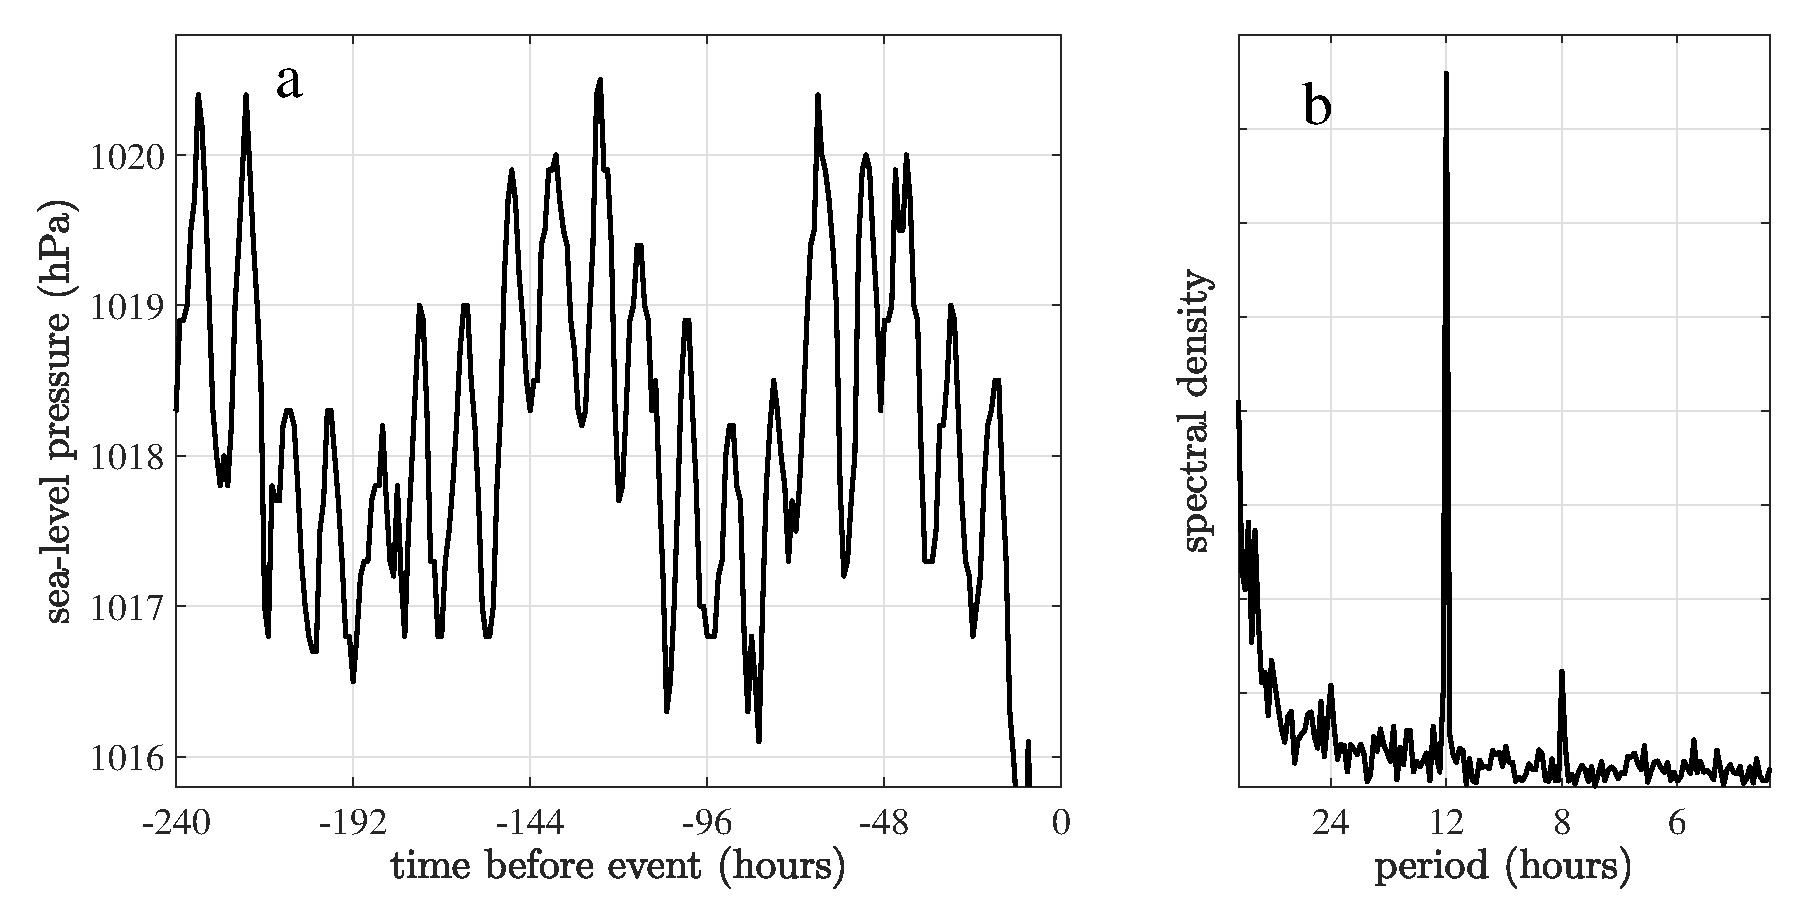
\includegraphics[width = 0.9\textwidth]{osc_and_powerspectrum}
		\caption{Sea-level pressure periodic oscillations. Panel \textbf{a}: A 240 hour segment of the sea-level pressure data preceding the Hurricane Andrew event, we note the 12-hour oscillations on the longer term fluctuations. Panel \textbf{b}: The periodogram obtained from a 35 day segment of the same time series (between 15 and 50 days before the event), we note the spike at 12 hours.
			\label{fig:TC:osc_and_powerspectrum}}
	\end{figure}
Two approaches were employed. First, a filtering approach where, given a time series $[Z]_k$ a deseasonalised series $[Z_\textrm{D}]_k$ is created according to the formula
	\begin{equation}
		Z_\textrm{D}(k) = Z(k)-\underset{_{i = k~\textrm{mod}12}}{\textrm{mean}}\left({Z(i)}\right).
		\label{eqn:TC:deseasonalise}
	\end{equation}
The other approach is to subtract a sine wave with 12 hour period, that is, a new series $[Z_\textrm{S}]_k$ is given according to
	\begin{equation}
		Z_\textrm{S}(k) = Z(k) - A\sin\left(\frac{2\pi}{12}(k - \phi)\right)
		\label{eqn:TC:subtractsinewave}
	\end{equation}
where $A$ is the mean amplitude found over the entire series, as described above, and $\phi$ is required to align the series $Z$ with the sine wave. In practice, the phase $\phi$ was found in each case by minimising the variance of $Z_\textrm{S}$ over values of $\phi\in[0,12)$. 

{\Red{
Both of these approaches are applied to pressure data from the Florida Keys station in the period of 50 to 15 days before the appearance of Hurricane Andrew, and for both of the new series, as well as the original raw series, the ACF1, DFA and PS indicators are calculated and the results are shown in figure~\ref{fig:TC:removeOsc}. In the calculation of the indicators, the sliding window used is $90$~points for ACF1, $90$~points for DFA, and $102$~points for PS; these window sizes are chosen according to the sensitivity analysis (see section~\ref{subsec:TC:1D_SA}) and are consistent with those used throughout this chapter.

We note that both methods of removing oscillations give almost identical results, both qualitatively and when considering the autocorrelation of the resulting series.

The effect on the ACF1 indicator is, effectively, of smoothing out the larger fluctuations but it does not appear to change the general shape of the indicator series (that is, longer scale increases or decreases). The same is true of the DFA and PS indicators, although in the case of the DFA indicator there is apparently some extra detail visible when using the filtered series (red and blue lines) which is not visible when using the original, oscillating data: specifically, there appears an increase in the DFA indicator (both red and blue lines) starting after $\m 600$ hours, which cannot be seen in the grey line. 

We suggest it may be beneficial, especially when using the DFA indicator, to first filter the tidal oscillations in the sea-level pressure data before attempting to produce an early warning signal. However, it is not apparently important whether the deseasonalising approach or sine-wave approach is used. For the remainder of this chapter, the deseasonalising approach (see equation~\ref{eqn:TC:deseasonalise}) is used whenever oscillations are removed from data in this way.



%For this reason the 12-hour oscillations in pressure were not removed in further analysis of the tropical cyclone data.
}}

\begin{figure}
	\centering
	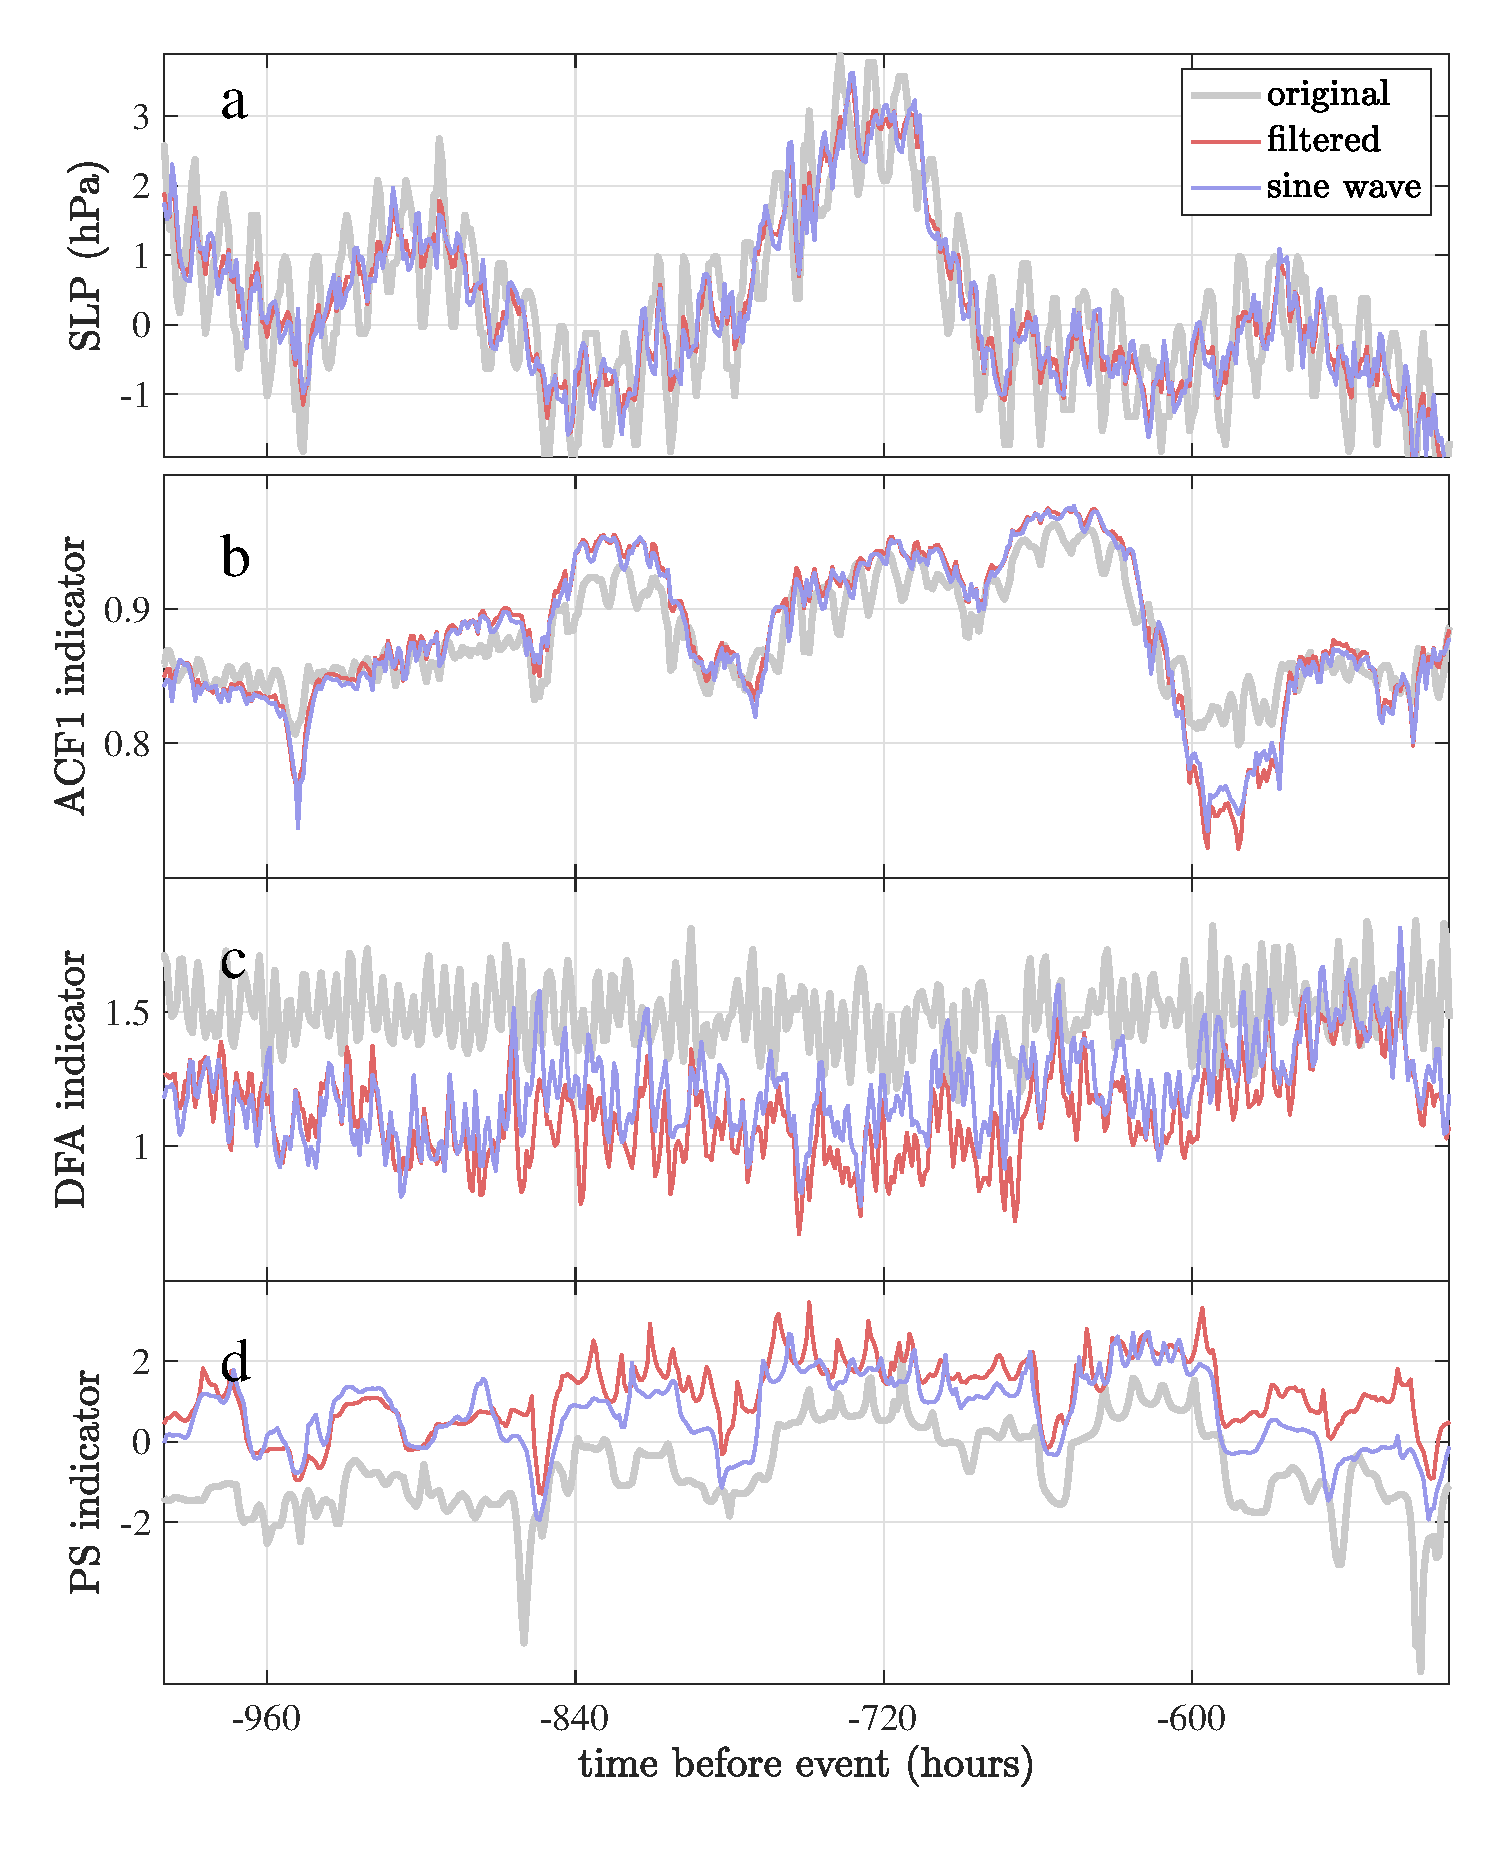
\includegraphics[width = 0.9\columnwidth]{removeOsc_all3}
	\caption{\Red{Sea-level pressure deviation from the mean at the Florida Keys station in a period from 15 to 50 days before Hurricane Andrew. Three time series are considered: the original raw data (grey line); the same data with oscillations removed by filtering (red, see equation~\ref{eqn:TC:deseasonalise}); and the data with oscillations removed by subtracting a sine wave (blue, see equation~\ref{eqn:TC:subtractsinewave}). Panel \textbf{a} shows the sea-level pressure deviation from the mean whilst panels \textbf{b}, \textbf{c} and \textbf{d} show the ACF1, DFA and PS indicators (respectively) of the three series.}}
	\label{fig:TC:removeOsc}
\end{figure}


\subsection{Evidence of scaling in the sea level pressure series}
\label{subsec:TC:evidenceOfScaling}

{\Red{
In figure~\ref{fig:TC:osc_and_powerspectrum} (page~\pageref{fig:TC:osc_and_powerspectrum}) we presented the periodogram of the sea level pressure time series from the weather station chosen for its proximity to the landfall location of Hurricane Andrew. Now, in figure~\ref{fig:TC:PS_loglog_RO12}, we present the periodograms from all fourteen stations chosen for each of the fourteen tropical cyclones detailed in table~\ref{tab:TC:14cyclones}. In each case we use a time series of length 2400 hours which terminates 96 hours before the cyclone event, so that this is not included. Additionally, the spike at the 12-hour period has been removed by removing the oscillations, as discussed in the previous section. The periodograms are plotted on a log-log scale so that a linear trend, which is evidence of power-law scaling, may be apparent. The periodograms are plotted in the frequency range $\m2\leq\log f\leq\m1$ since this is the range used for the estimation of the PS exponent.

We note that in some cases there appears to be definite power-law scaling, such as in the example of Flo (top left panel), whereas other periodograms appear to contain crossovers in the given frequency range, or show little evidence of any correlation. In general the periodograms show a negative linear gradient as expected in correlated (red noise) signals. 

As we have remarked in section~\ref{subsec:1D:Exponents_as_EWS:nopowerlawsacaling}, the estimation of the PS exponent for use as the PS indicator does not assume power-law scaling and merely seeks to detect a `reddening' of the signal, which is present even in systems such as the AR(1) process which do not exhibit true power-law scaling in the asymptotic. 
}}

\begin{landscape}
	\begin{figure}
		\centering
		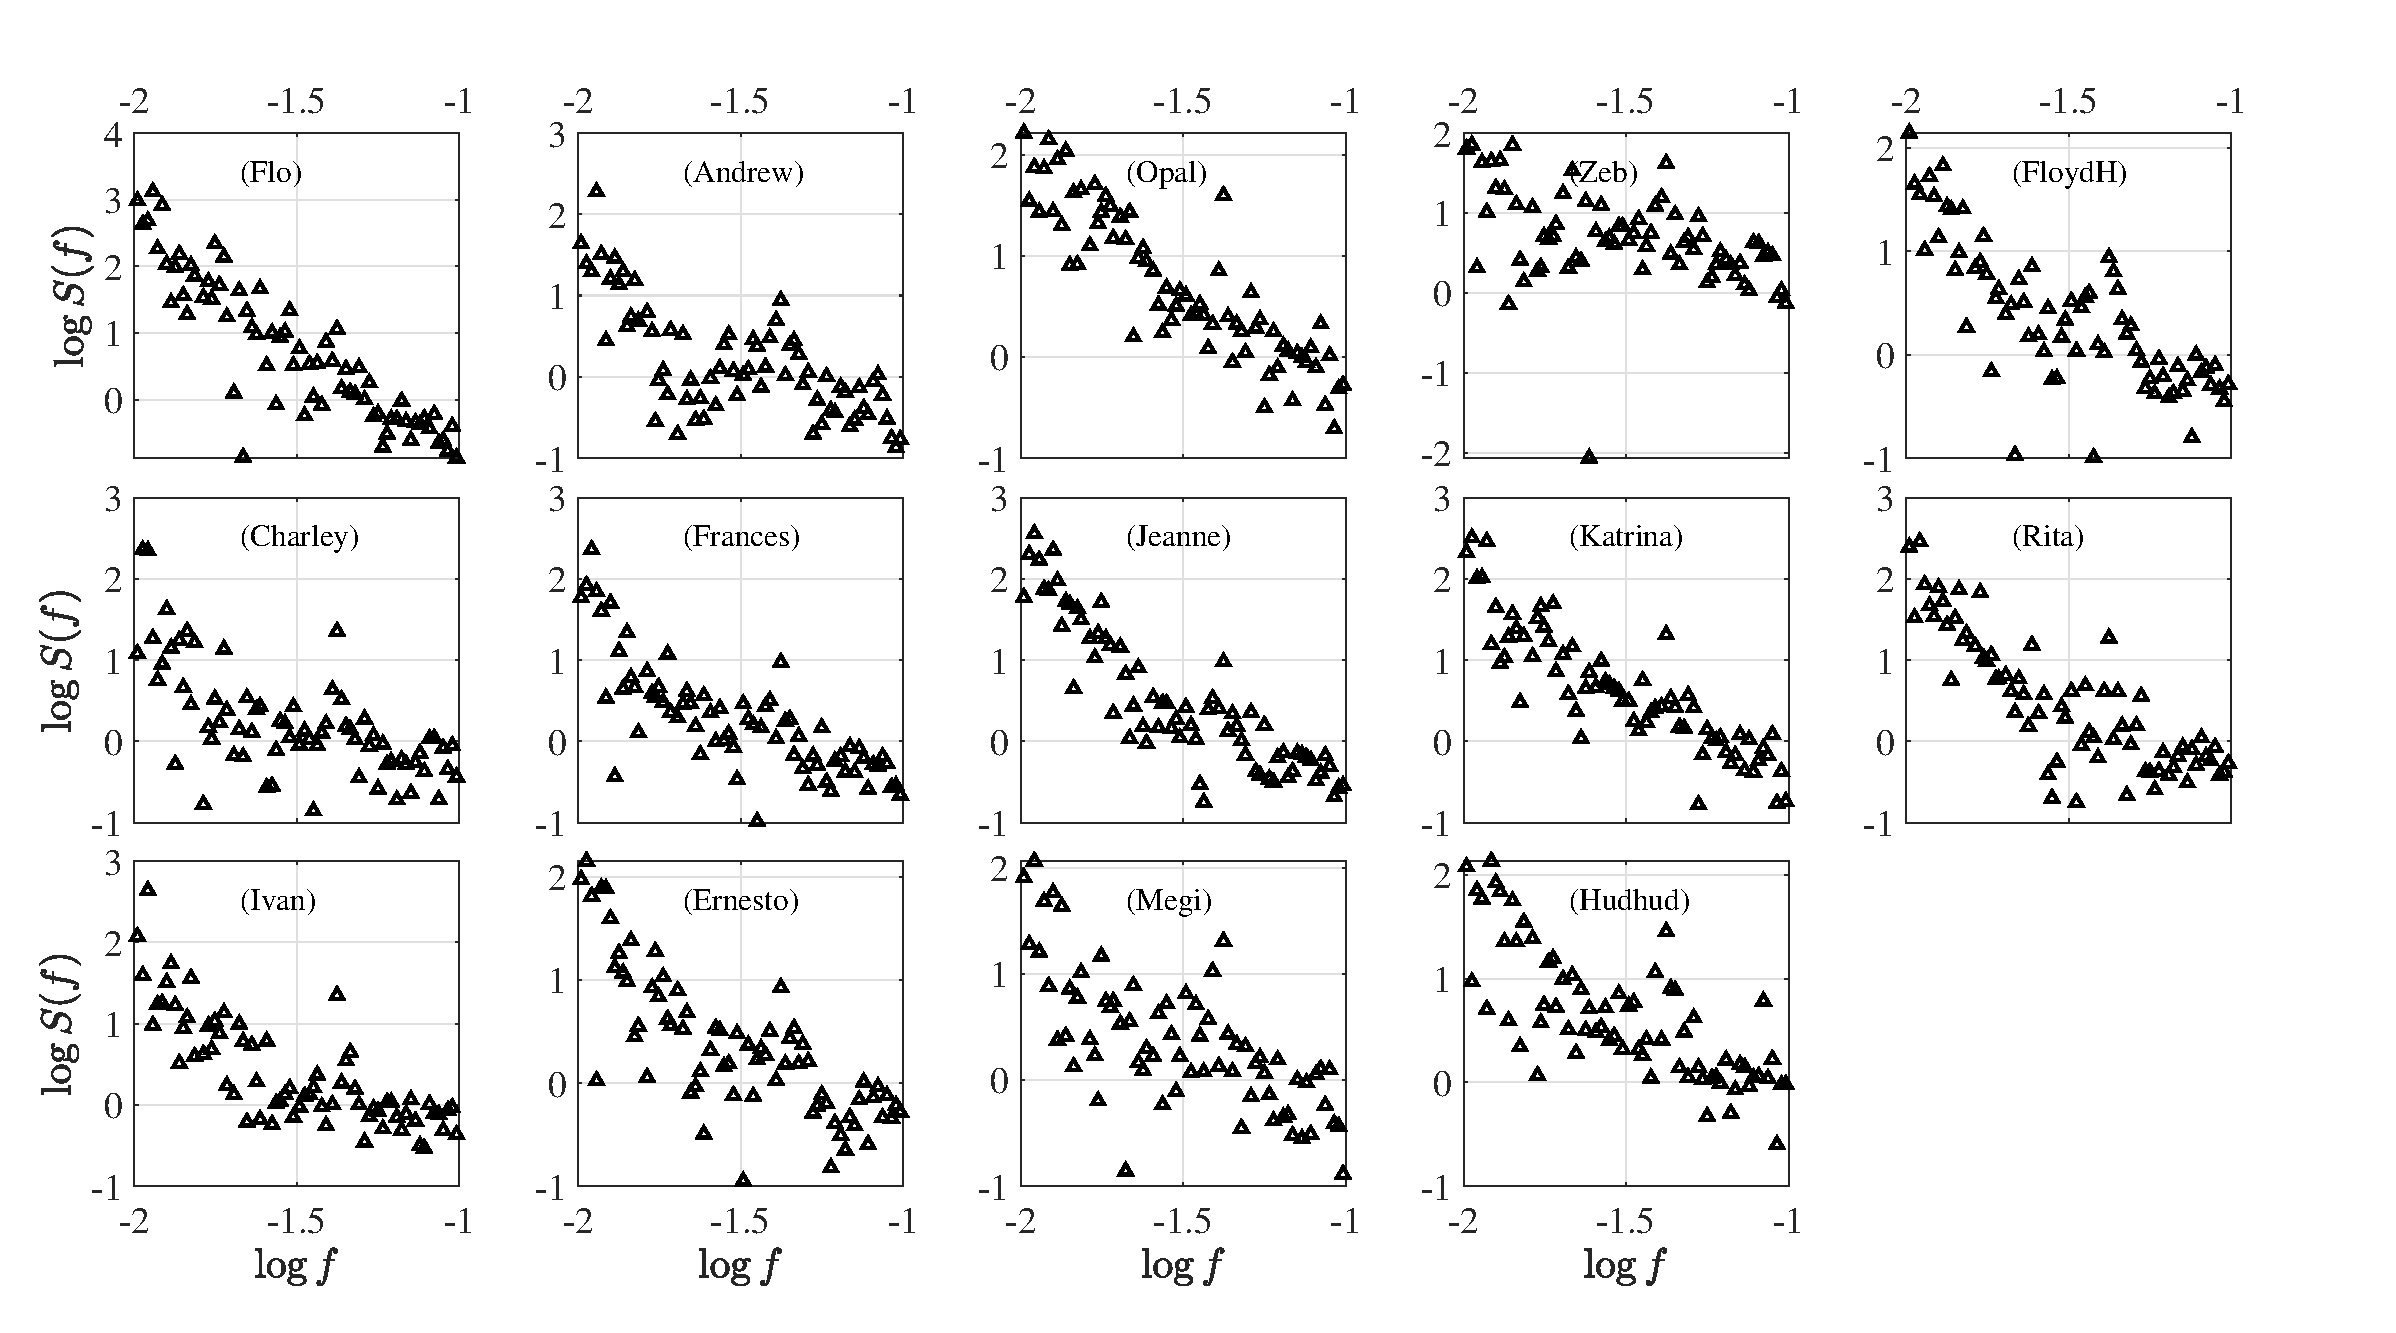
\includegraphics[width=\linewidth,keepaspectratio]{PS_loglog_RO12}
		\caption{\Red{The periodogram for each of the sea level pressure series from weather stations chosen for each of the fourteen tropical cyclones detailed in table~\ref{tab:TC:14cyclones}. In each case we use a time series of length 2400 hours which terminates 96 hours before the cyclone event, and the 12-hour period oscillations have been removed.
		}}
		\label{fig:TC:PS_loglog_RO12}
	\end{figure}
\end{landscape}


\section{Application of one-dimensional tipping point techniques}
\label{sec:TC:1Dtechniques}

In this section we consider the time series of the sea-level pressure variable at a fixed location in the time immediately before the arrival of a tropical cyclone in that location. We use the fourteen tropical cyclones that are detailed in table~\ref{tab:TC:14cyclones} (see section~\ref{subsec:TC:data:HadISD}). 

In the case of each of the fourteen cyclones, the sea-level pressure time series is centred on the minimum pressure value which is labelled $t=0$. This cannot be called analogous to the bifurcation point in the pitchfork bifurcation example of chapter~\ref{chap:1D}  (figure~\ref{fig:1D:pitchforkEWS}, page~\pageref{fig:1D:pitchforkEWS}) but is a common feature of all time series which is convenient to use for the purpose of comparison. {\Red{The results presented in this section have previously been published in \cite{prettyman2018}.}}

\subsection{Method}
\label{subsec:TC:1Dmethod}

The same methods are applied to the sea-level pressure time series here as are applied to the model examples in section~\ref{sec:1D:indicatorComparison}. The ACF1, DFA and PS indicators {\Red (definitions \ref{def:1D:indicator:ACF1}, \ref{def:1D:indicator:DFA} and \ref{def:1D:indicator:PS} respectively, see section~\ref{sec:1D:Exponents_as_EWS}, page~\pageref{sec:1D:Exponents_as_EWS}) } are applied to the times series with a sliding window of approximately 100 points, equivalent to 100 hours in this data. The exact window sizes used, for each indicator, are: ACF1: $90$~points; DFA: $90$~points; PS: $102$~points. These values are determined by the sensitivity analysis which will be explained in section~\ref{subsec:TC:1D_SA}. Each of the three indicator series is calculated for each of the fourteen time series and then the mean over these fourteen series is calculated.

\begin{figure}
	\centering
	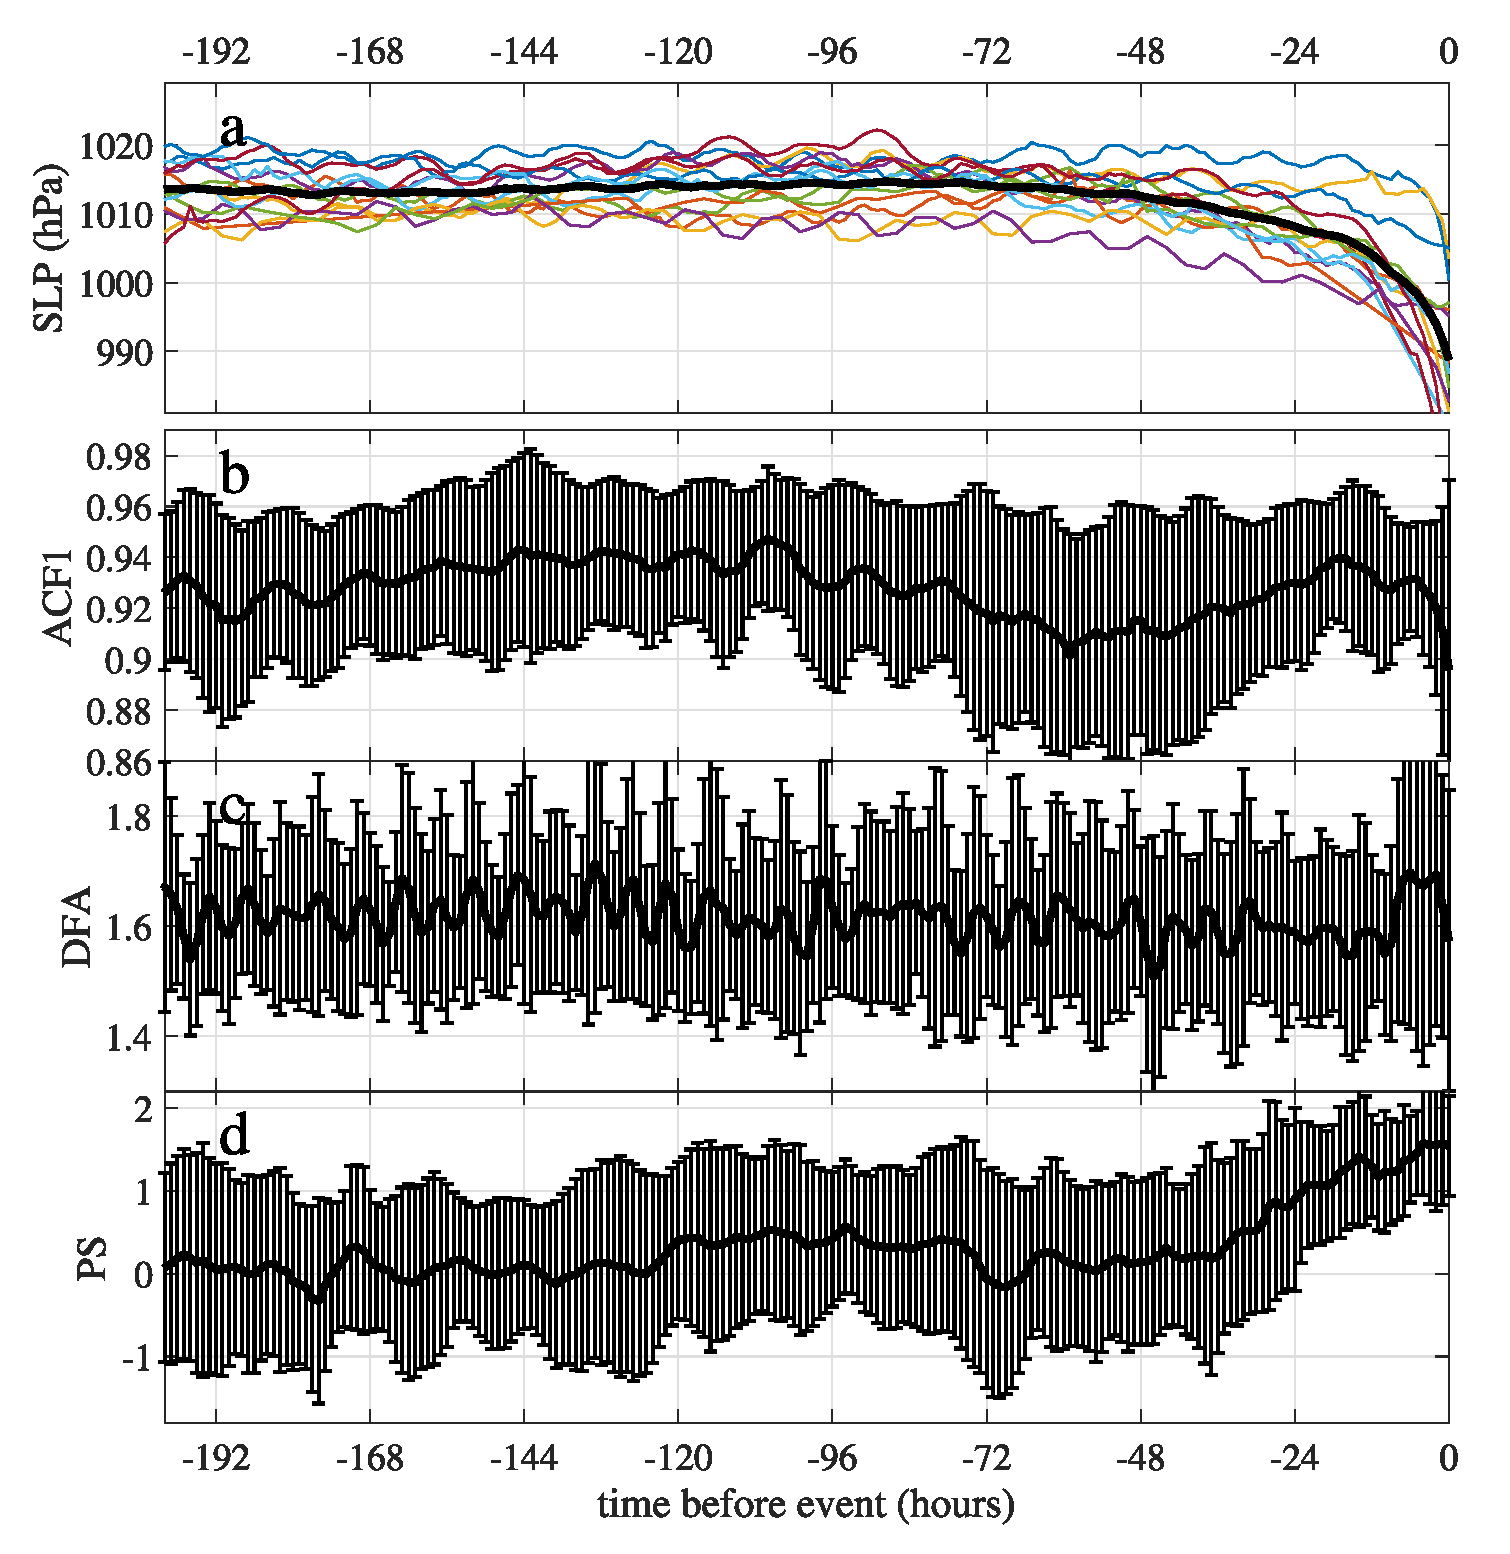
\includegraphics[width = 0.9\textwidth]{indicators14_slp}
	\caption{ACF1, DFA and PS indicators applied to sea-level pressure data. Panel {\bf a}: Data from the 14 tropical cyclones, mean shown in black. Panels {\bf b}, {\bf c}, {\bf d}: The mean ACF1, DFA and PS indicators, with error bars of 1 standard deviation. The ACF1 indicator does not provide a clear EWS in this case. The DFA indicator shows a small, sudden increase just before the event. The PS indicator begins to rise around 48 hours before the cyclone event. \label{fig:TC:1DindicatorsSLP}}
\end{figure}

\subsection{Results}
\label{subsec:TC:1Dresults}


Figure~\ref{fig:TC:1DindicatorsSLP} shows the fourteen sea-level pressure time series centred at the point of minimum pressure (panel \textbf{a}) and the mean of the three indicator series (ACF1, DFA and PS indicators in panels \textbf{a}, \textbf{b} and \textbf{c}). The mean indicator series are shown with error bars of one standard deviation. 

We note that the ACF1 indicator is consistently high (greater than $0.9$) over the entire series and does not apparently rise as a precursor of the cyclone event. The mean of the DFA indicator increases within the time period that the drop in pressure is obvious in the time series (24 hours before the event), and so the increase cannot be said to be an early warning signal. The PS indicator, however, does show an increasing trend starting at around 50 hours before the minimum pressure, although it is not significant at the level of one standard deviation. 

{\Red{We note that the consistently high value of the ACF1 indicator may be due simply to the one-hourly sampling rate of the data points. By using a different autocorrelation lag we can compensate for this effect by simulating different sampling rates, in which case an EWS may be visible. In figure~\ref{fig:TC:ACF_lags_comp} we repeat the same experiment as before but instead of using the ACF1, DFA and PS indicators, we use the ACF1, ACF2, ACF3, etc. indicators corresponding to using a higher-lagged autocorrelation function. The results are presented for lags 1, 2, 3, 4, 5, 6, 8, 10 and 12. We see that a better EWS is visible in the lag-4 autocorrelation indicator than in the previously-used ACF1. In figure~\ref{fig:TC:ACF_lags_comp_RO} we present the same results again but, in this case, the oscillations have been removed from the sea-level pressure data as explained in section~\ref{subsec:TC:data:oscillations}. Again, we see that removing the oscillations does not appear to improve performance of the EWS indicators in this example, even when using lag-4 autocorrelation. 
}}

\begin{landscape}
	\begin{figure}
		\centering
		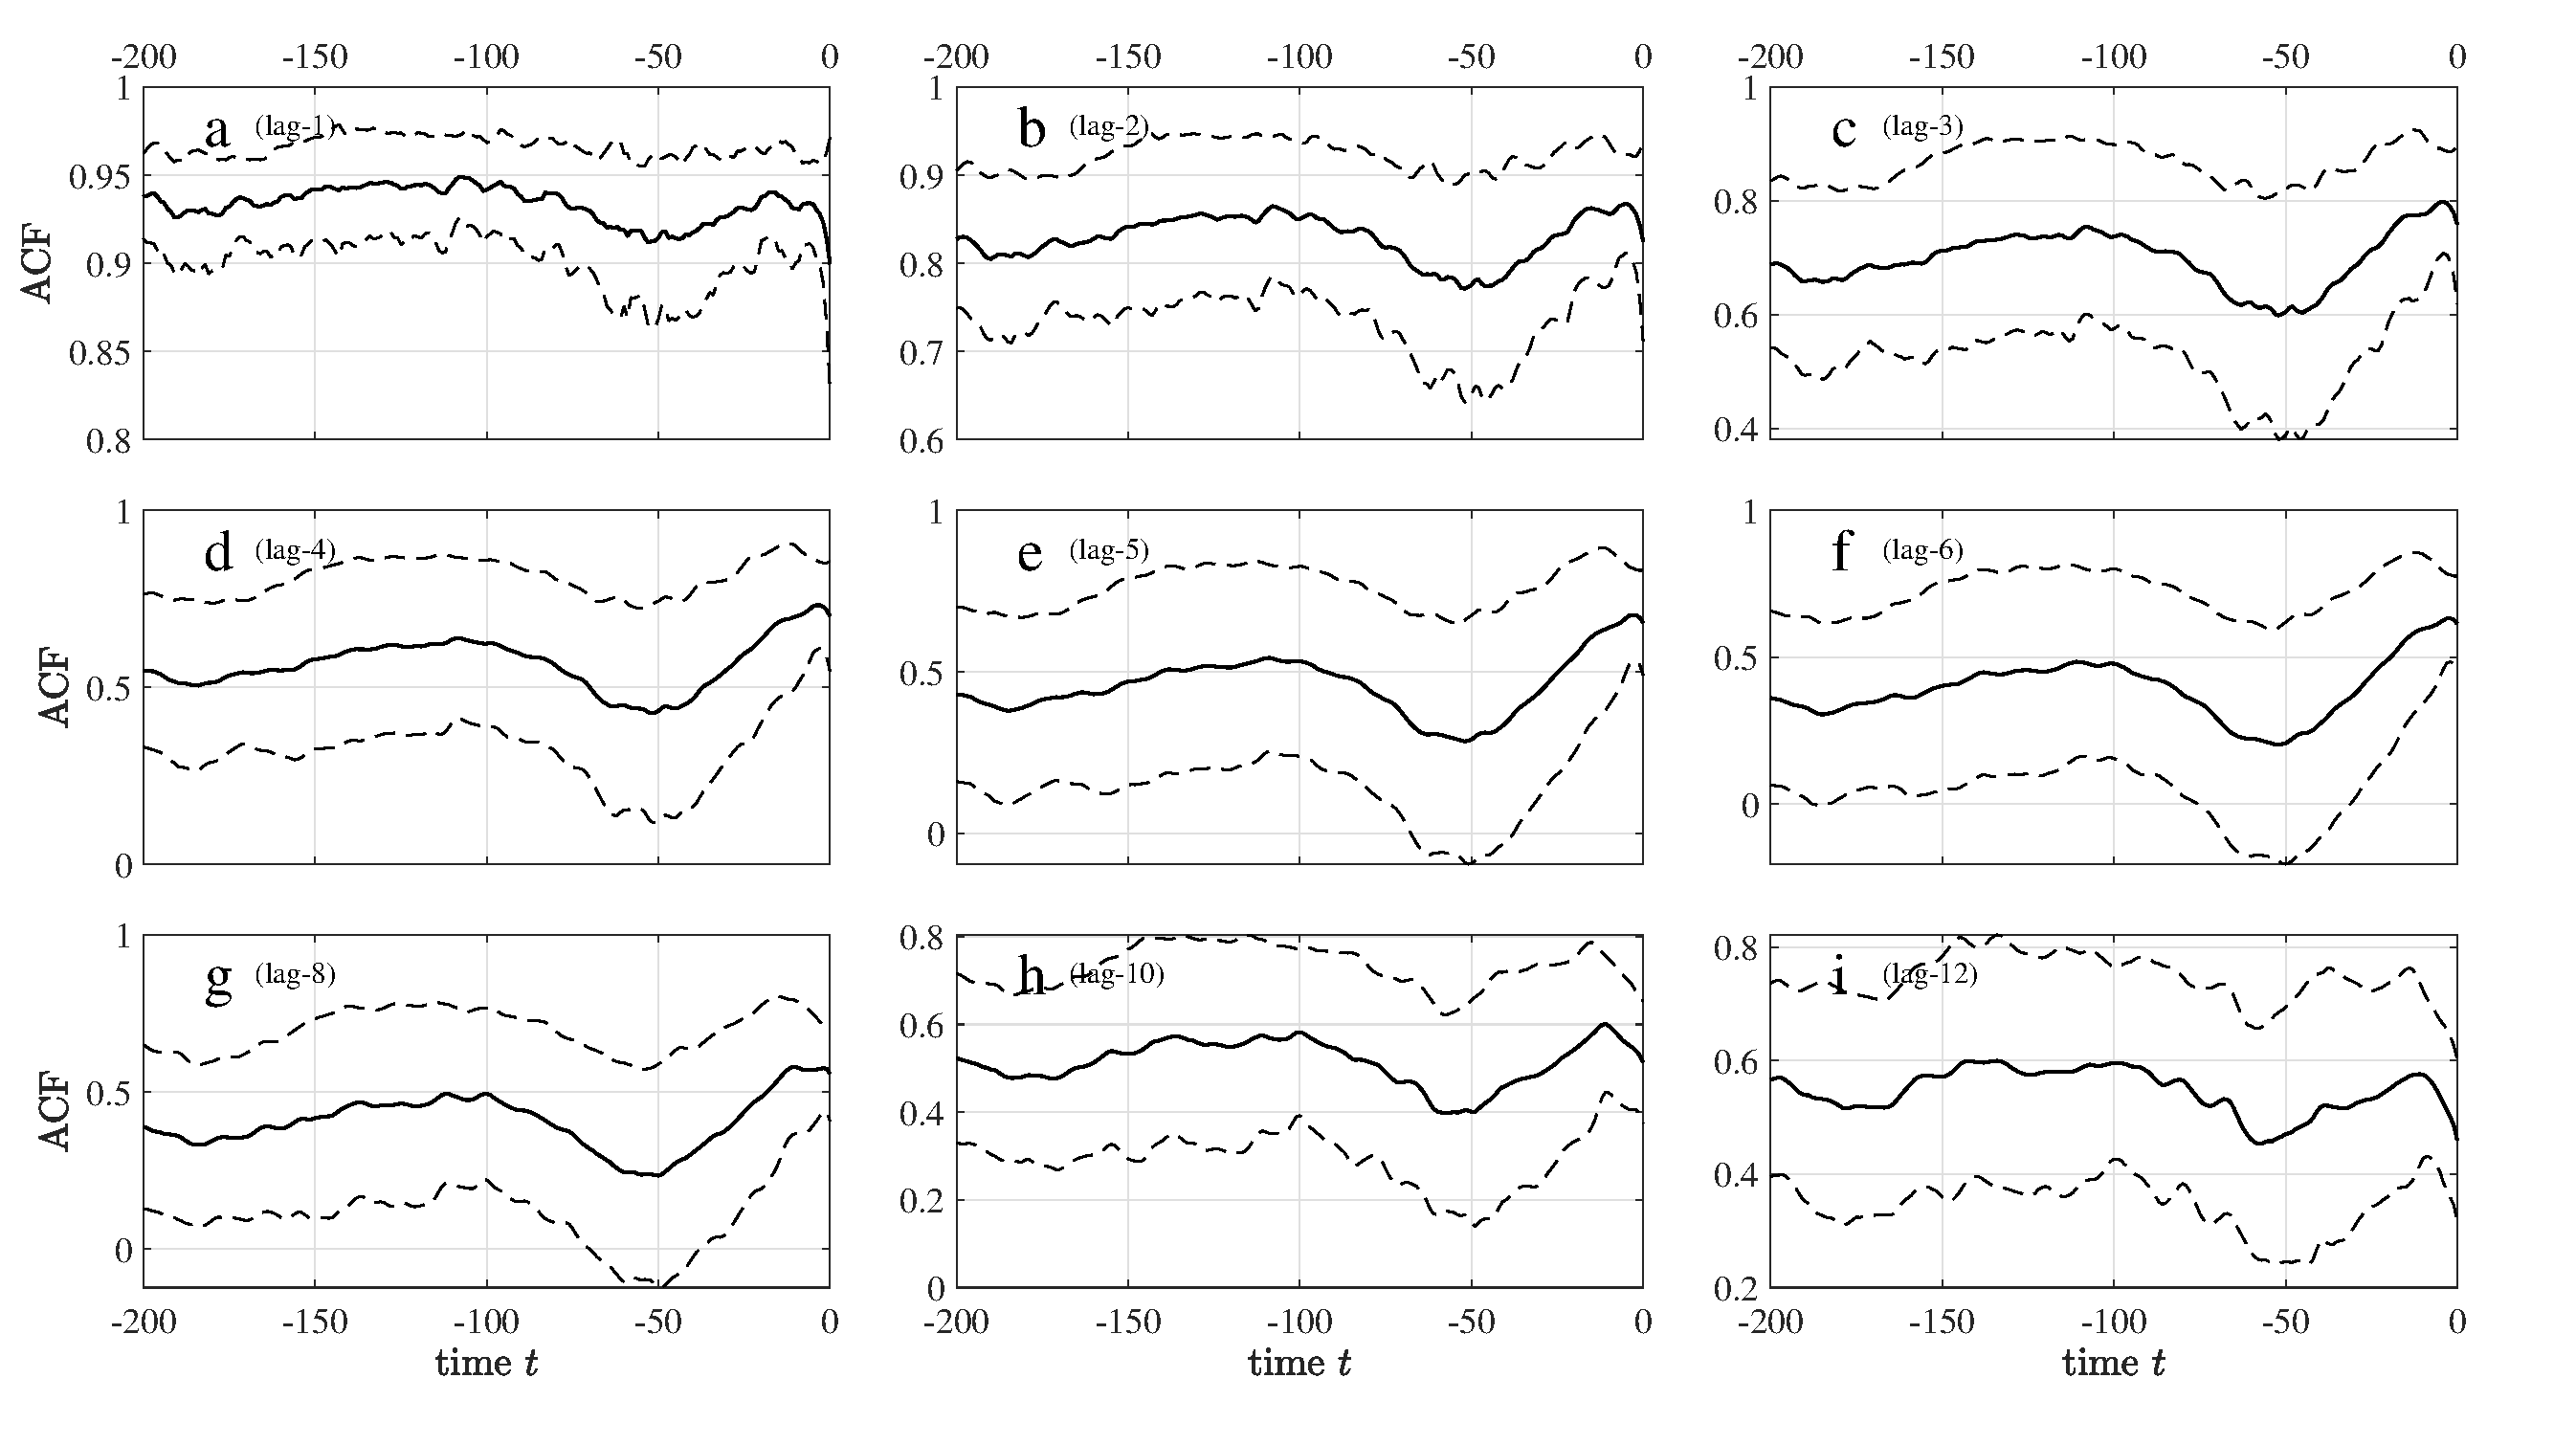
\includegraphics[width=\linewidth,keepaspectratio]{ACF_lags_comp}
		\caption{\Red{The ACF indicator is applied to the sea-level pressure time series of the fourteen tropical cyclones using an autocorrelation function with lags 1, 2, 3, 4, 5, 6, 8, 10 and 12 (in panels {\bf a}-{\bf i} respectively). The best EWS is visible when using a lag-4 ACF. }
		}
		\label{fig:TC:ACF_lags_comp}
	\end{figure}
\end{landscape}

\begin{landscape}
	\begin{figure}
		\centering
		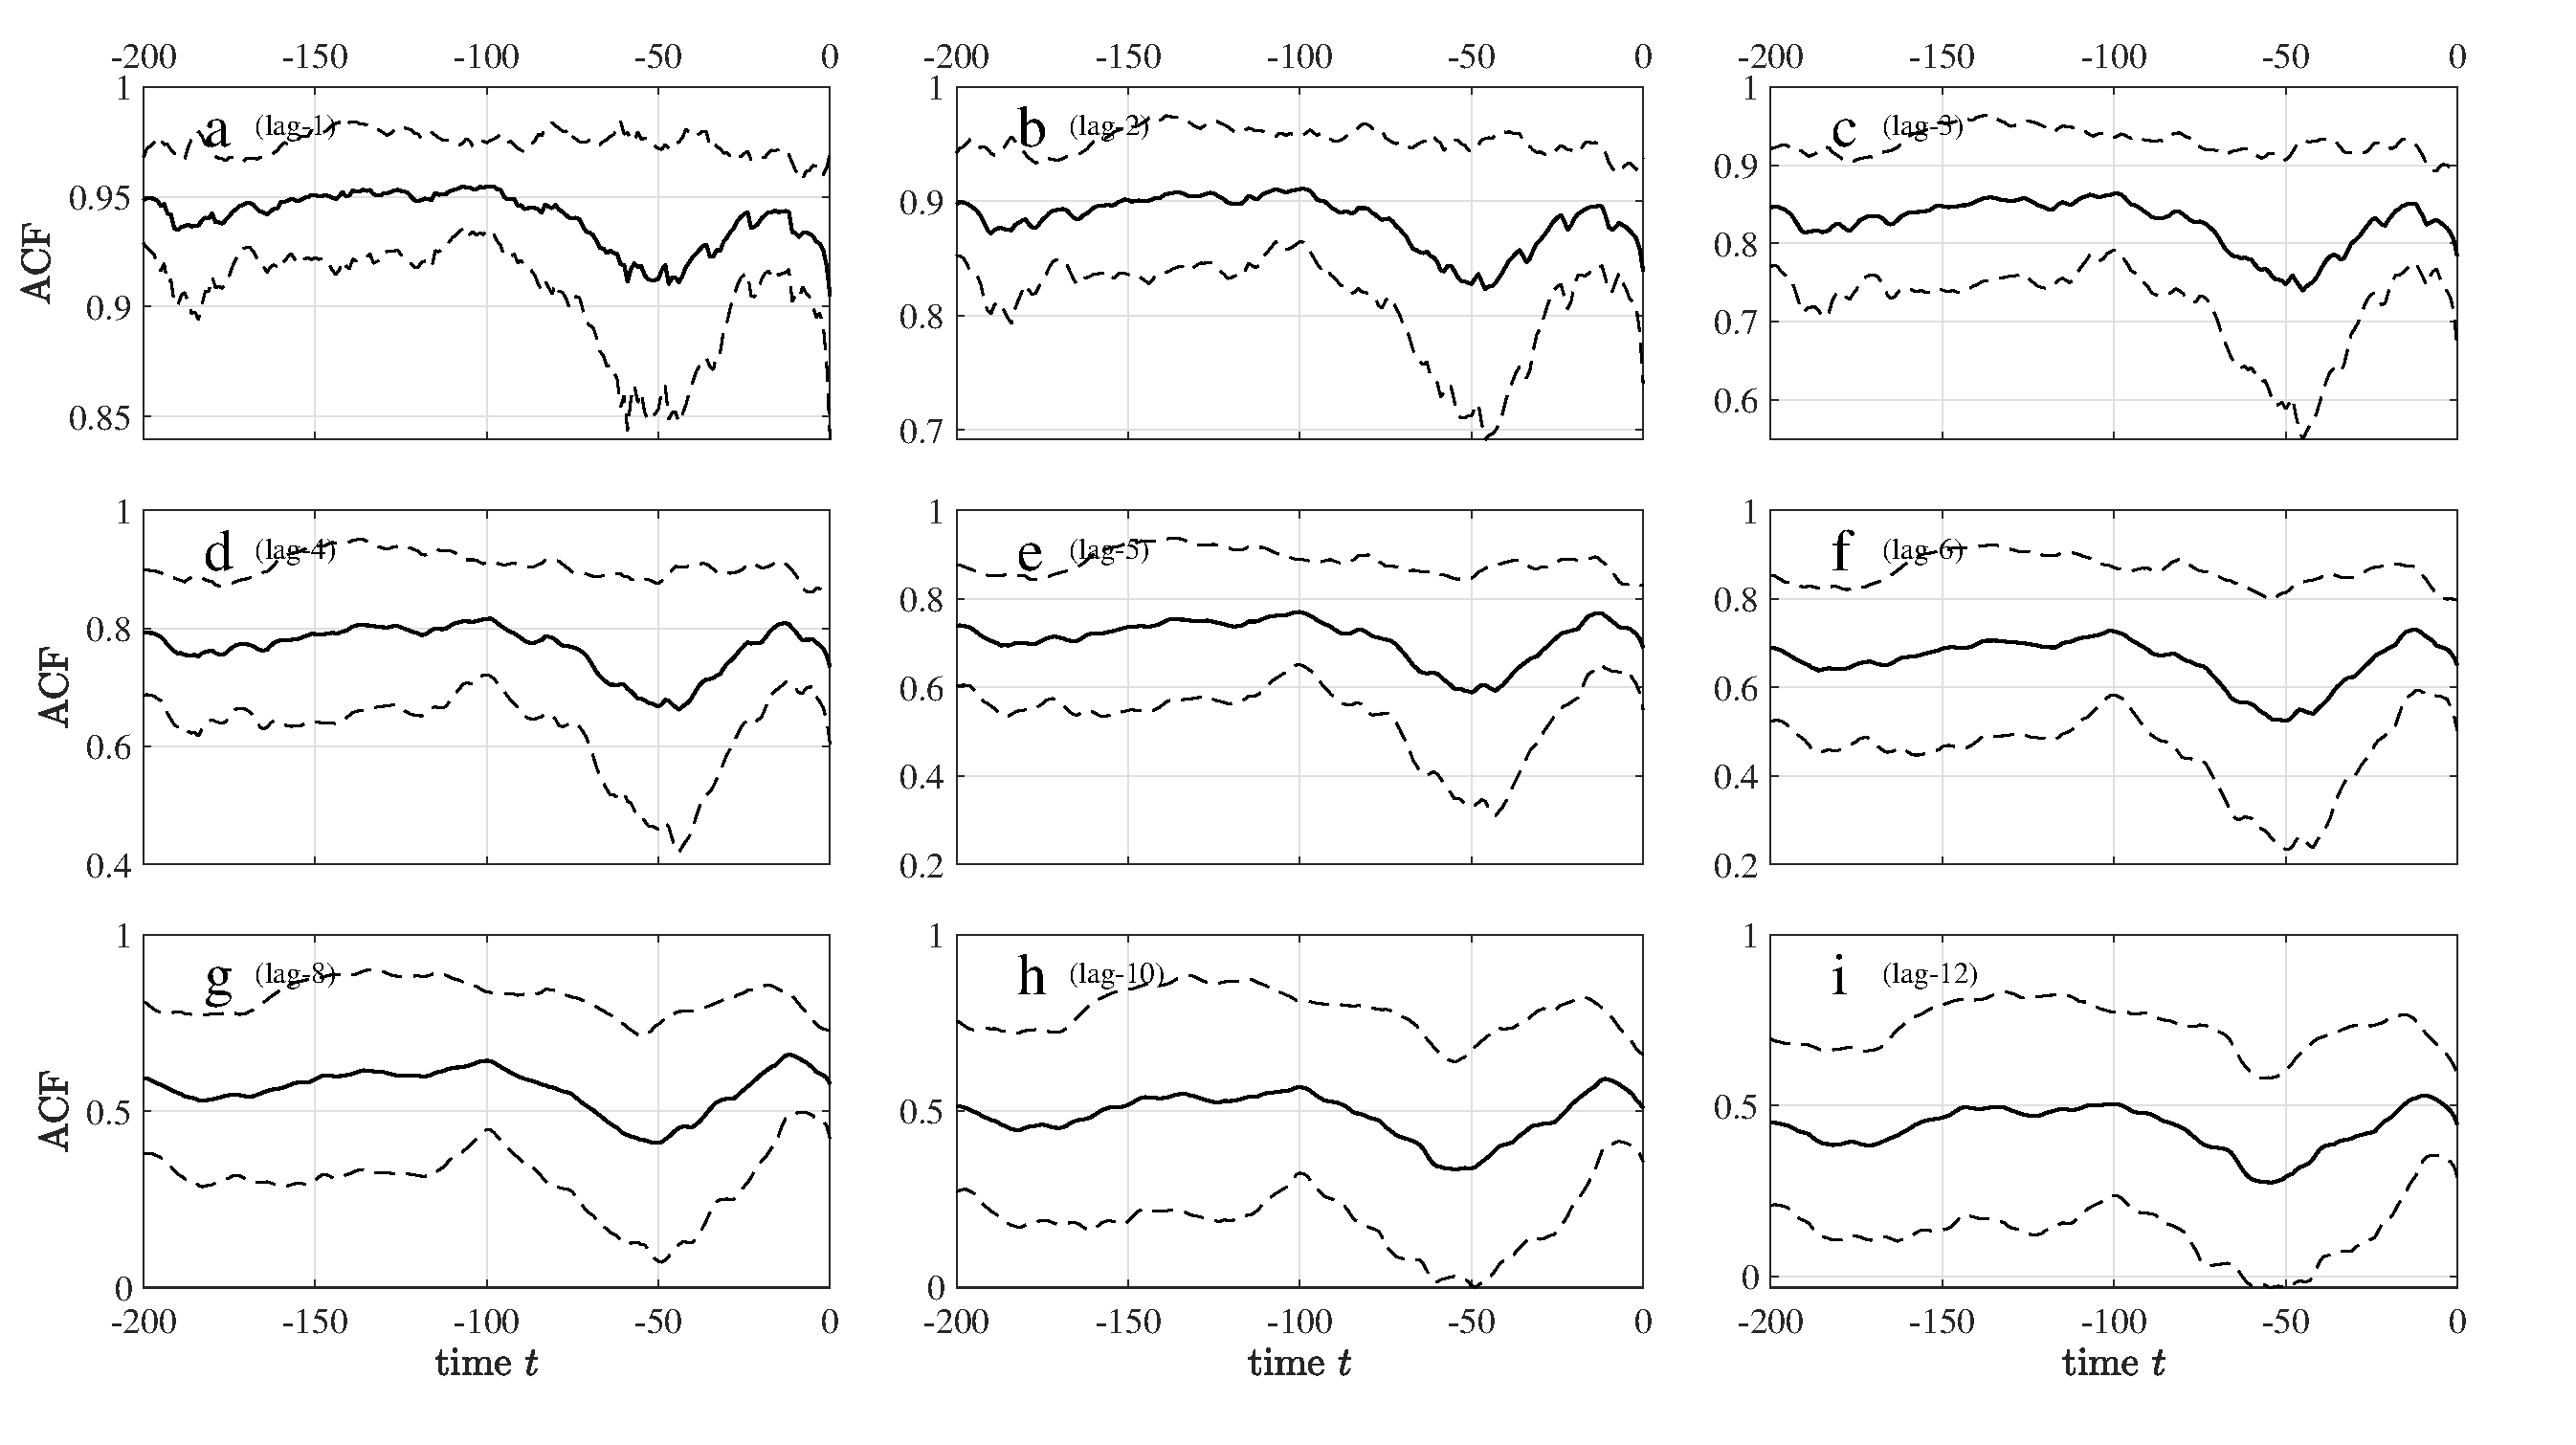
\includegraphics[width=\linewidth,keepaspectratio]{ACF_lags_comp_RO}
		\caption{\Red{A repeat of the method presented in figure~\ref{fig:TC:ACF_lags_comp}, but the oscillations have been removed from the sea-level pressure data as explained in section~\ref{subsec:TC:data:oscillations}. Again, the ACF indicator is applied to the sea-level pressure time series of the fourteen tropical cyclones using an autocorrelation function with lags 1, 2, 3, 4, 5, 6, 8, 10 and 12 (in panels {\bf a}-{\bf i} respectively). }
		}
		\label{fig:TC:ACF_lags_comp_RO}
	\end{figure}
\end{landscape}

\subsection{Sensitivity analysis}
\label{subsec:TC:1D_SA}

In order to calculate the indicator series shown in figure~\ref{fig:TC:1DindicatorsSLP}, it is necessary to select an appropriate window size. The calculation of each of the indicator series requires an appropriately large window size in order to yield an accurate calculation of the scaling exponent. The calculation of the power spectrum scaling exponent from the periodogram obtained using the fast Fourier transform is particularly inaccurate when only a small number of points are available. 

Besides the error due to the noise in the periodogram, the actual periodic spikes in the periodogram, such as the spike representing the 12-hour oscillations, have a greater influence on the calculation of the scaling exponent when fewer points are used. Furthermore, the calculation of the DFA exponent requires a minimum number of points depending on the parameters selected. The lag-1 autocorrelation could reasonably be calculated for a series of only three points, but the ACF1 indicator exhibits large variability, as with the PS and DFA indicators, for small window sizes.

It is therefore desirable to use a sufficiently large number of points to give an accurate estimate of the scaling exponent with less noisy temporal variability. However, one must attain a compromise against the competing requirement for a short time window corresponding to the time scale of the phenomenon under investigation. For example, when we consider the sea-level pressure time series in figure~\ref{fig:TC:1DindicatorsSLP} we note that the visible influence of the cyclone on the pressure begins only around 24 hours before the minimum. When attempting to detect an early warning signal, using an indicator series calculated with a window of several weeks would clearly not be useful: the large number of points relative to the actual period of interest will smooth out any significant increase or decrease. There is also a limit imposed by the length of the time series data. We require a window size such that the indicator variance is significantly small that we can see the EWS, but that the rise in the indicator value before the tipping event is large enough so that we can recognise it as an EWS.

Here we analyse the sensitivity of each indicator to the window size used, in order to ascertain the optimal window size in this particular example of a physical phenomenon, if such a universal optimum exists.

We expect that the EWS apparently becomes stronger with decreasing window size, above a certain size where the variability becomes so large that it is not possible to detect an EWS. In this way, we make a subjective choice as to the optimum window size to use in this context. The hypothesis is that all cases considered here (all fourteen cyclones and their corresponding sea-level pressure time series) are sufficiently similar in the way that the scaling exponents behave that a general optimum (or near-optimum) window size exists. In this case, it will be possible to apply these indicator methods to new data from similar sources.

It is useful to produce a contour plot of the mean value of the indicator over time, with window-size on the $y$-axis. In this way we are able to visualise hundreds of indicator series simultaneously. In figure~\ref{fig:TC:PS_sensitivity} we present the PS indicator series calculated for window sizes from 40 points to 160 points. We see that there is an increasing trend in the PS indicator towards the end of the time series with almost all window sizes. The exceptions occur periodically where the window size is a multiple of twelve: using these window sizes the indicator has a high value ($\approx1.5$) over the entire series. The most obvious early warning signals occur with window sizes which are an odd multiple of $6$, that is, 90, 102, 114, etc.. Using larger values (e.g. 174) the useful variability in the indicator is smoothed out so that the trend towards the end of the series is less obvious. We hypothesise that this 12-hour pattern is created by the 12-hour oscillations present in the sea-level pressure data, which particularly influences the power spectrum (the pattern is not observed in the ACF1 and DFA indicators, see figures~\ref{fig:TC:ACF1_sensitivity} and~\ref{fig:TC:DFA_sensitivity}). We also observe that there is a qualitative change in the nature of the pattern as the window size is increased from 99 points to 100 points, at which point, on the $y$-axis, all of the contour lines are lined up horizontally. This observation has been mentioned to the team behind the HadISD dataset, namely the authors of \cite{HadISD_dunn16}, and it has been ruled out that this is an artefact of the data collection or filtering. The investigation of the cause of this effect may be a topic for future work involving the PS indicator applied to sea-level pressure data. The 12-hour pattern serves to highlight the necessity of considering such sensitivity of the method to the window size parameter.

\begin{figure}
	\centering
	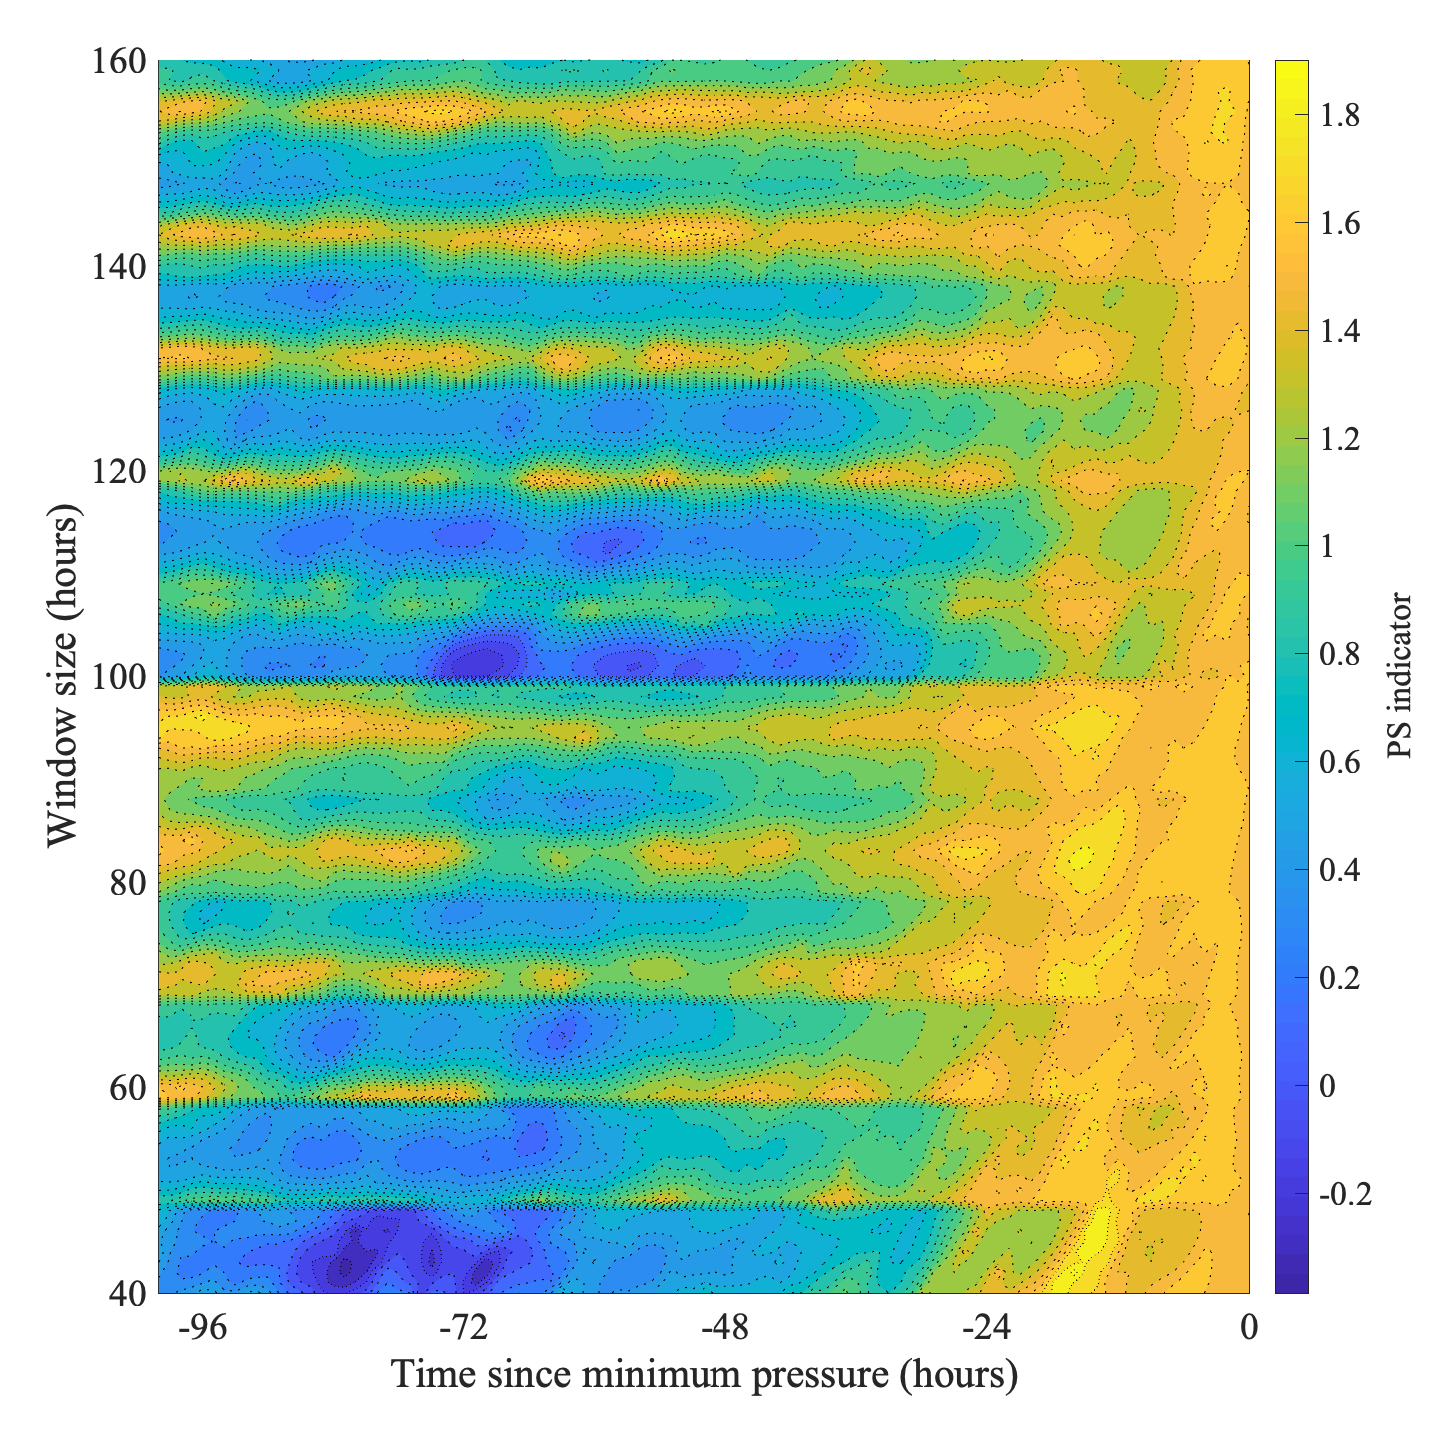
\includegraphics[width = 0.9\textwidth]{PS_sensitivity_mean}
	\caption{Mean over 14 tropical cyclones of PS indicator of the SLP data (see fig. \ref{fig:TC:1DindicatorsSLP}) calculated using window sizes from 40 to 160. The PS indicator appears to rise around 40 hours before the cyclone event in almost all cases, the exceptions occur when the window size is a multiple of 12, in these cases the indicator is high (greater than $1$) over the entire series. \label{fig:TC:PS_sensitivity}}
\end{figure}

We hypothesise that a time scale of about 100 hours, or four days, is a cut-off for the study of tropical cyclone in the context of early warning signals. A longer window encompasses too much of the time series before any forewarning signal is created, that is, before the cyclone has any influence on the autocorrelation of the sea-level pressure. Since the data available is hourly, this promotes an unfortunately short window of 100 points or fewer, which introduces a large amount of variability into the indicator series due to noise-sensitivity in the scaling exponent calculations. For this reason we proceed, in sections~\ref{sec:TC:2Dtechniques} and~\ref{sec:TC:field_data}, to incorporate more data into the calculation of a tipping point indicator series.

In keeping with the decision to select a window size of about 100 points, we selected a window size of 102 points when calculating the PS indicator in figure~\ref{fig:TC:1DindicatorsSLP}. At 90 points, the indication does not provide such an obvious early warning signal. In figure~\ref{fig:TC:PS_windows_indicators} we present the PS indicator, as in figure~\ref{fig:TC:1DindicatorsSLP}d, but using window sizes of 54, 90, 102 and 150 points (in panels \textbf{a}, \textbf{b}, \textbf{c} and \textbf{d} respectively). Since the fast Fourier transform periodogram is a less accurate approximation of the power spectrum when using fewer points, we might expect there to be greater variability when using a short window: both less agreement between the fourteen time series, and more variability within each individual time series along the time scale. We observe, in figure~\ref{fig:TC:PS_windows_indicators}, that the former is not apparently the case: the size of the error bars, which is one standard deviation over the fourteen sea-level pressure series, is largest when using a window size of 102 points, which is our chosen value based on the more obvious early warning signal in the mean. 

In figure~\ref{fig:TC:stdSensitivity} we investigate in what way the variance in the indicator series is effected by the window size. We expect, since the estimation of the DFA and PS scaling exponents is less accurate for shorter time series, that using a shorter window would result in a noisier indicator series, regardless of the nature of the input data. For each window size we calculate the standard deviation in the indicator series for each of the fourteen tropical cyclones, then take the mean of the fourteen values of standard deviations. The indicator series is calculated between 300 hours and 48 hours before the event, so that any anticipated increase prior to the event (in the 48 to 0 hours range) is not confused with noise. The hypothesis proves correct for the DFA indicator, shown in red, until the window size reaches around 100 points, after which the standard deviation remains constant. For the PS indicator, the standard deviation also decreases with increasing window size, as expected, but jumps up again for window size 100 points, after which it continues to decrease steadily. This jump is presumably related to the qualitative change in the mean which also occurs at window size 100 points (see figure~\ref{fig:TC:PS_sensitivity}). As we have remarked above, it is not know why this occurs but the investigation of the effect is an interesting topic of future work. 

The PS indicator series is less noisy for window size 90 points, and also has less variability across the fourteen cyclones, than for 102 points. However, this must be balanced by the consideration that the early warning signal, if present at all, is more obvious in the 102 point window series. 

\begin{figure}
	\centering
	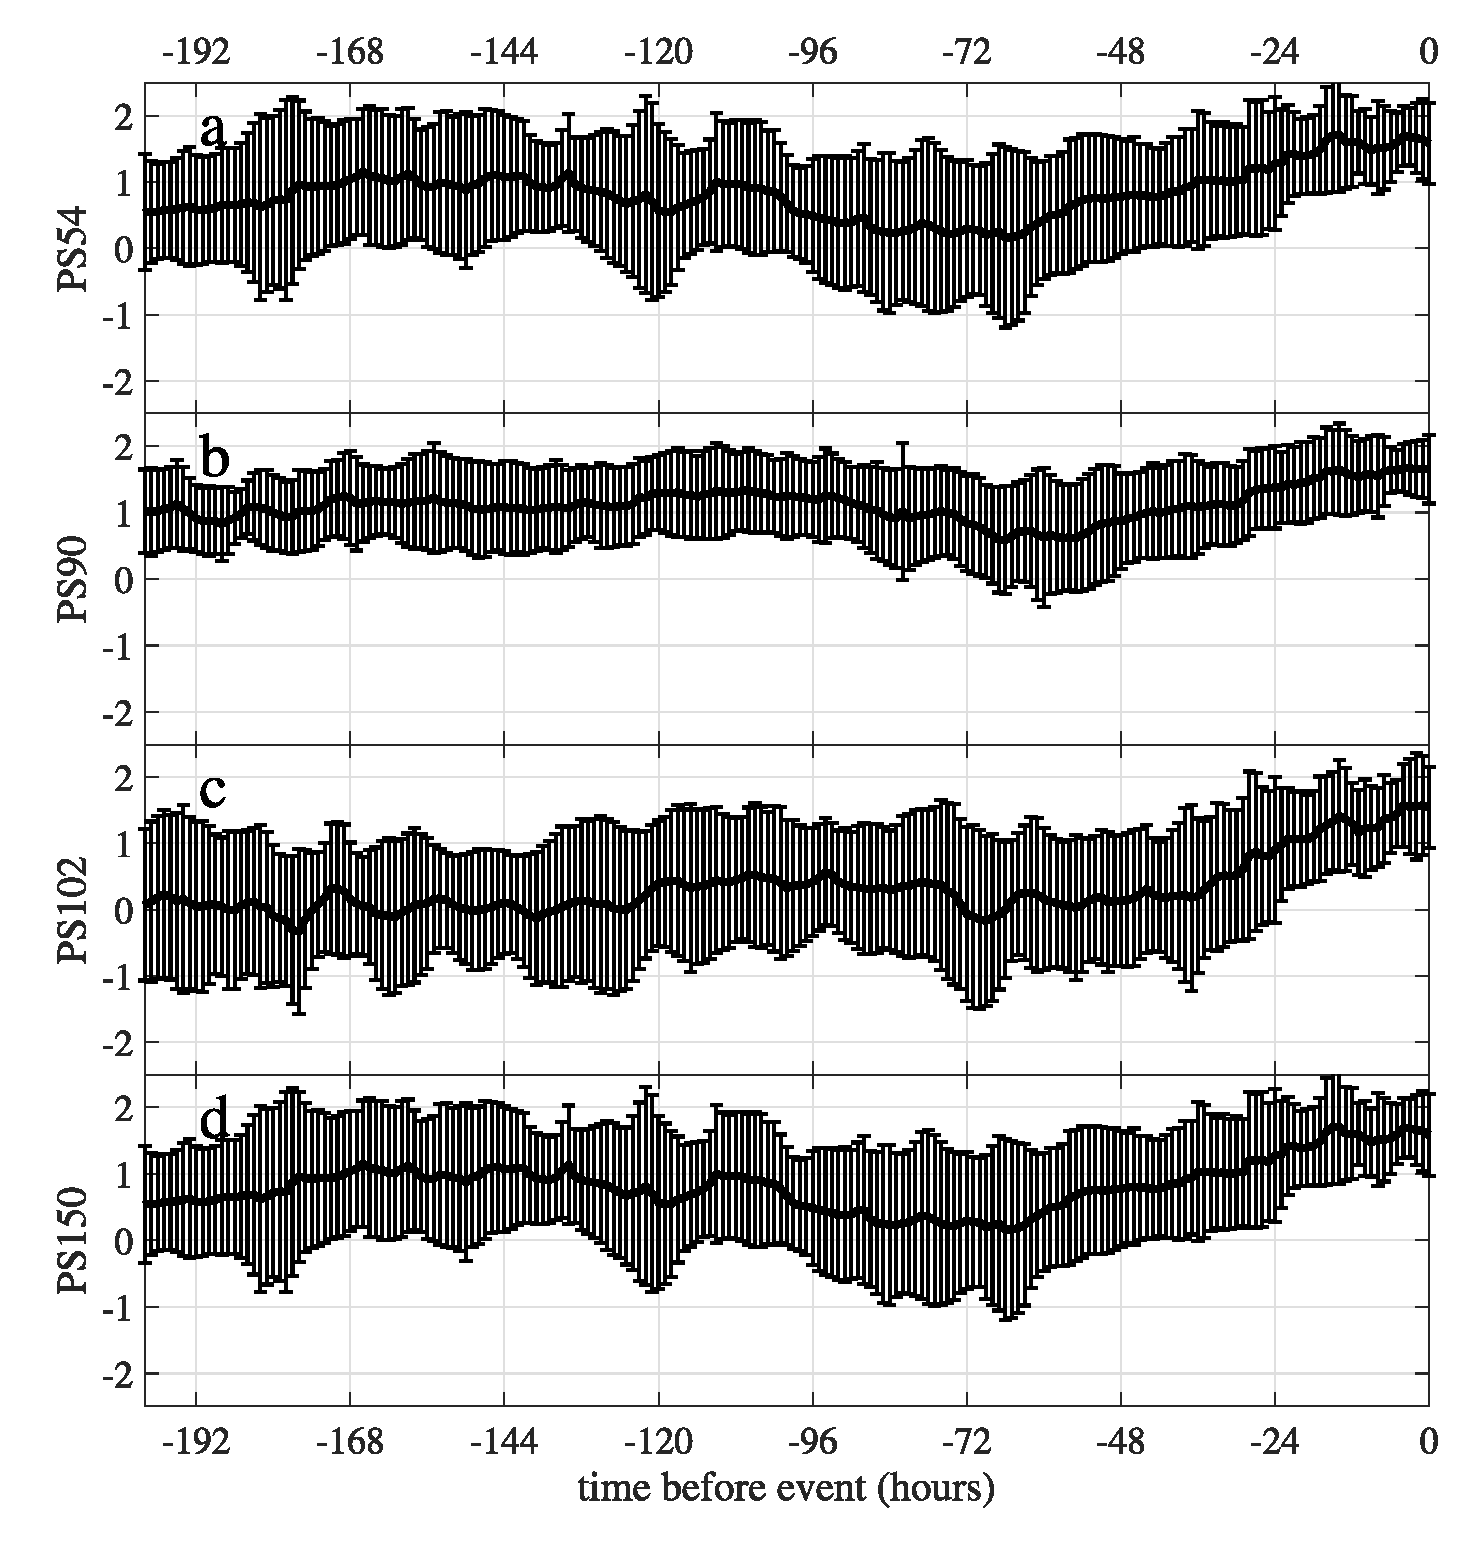
\includegraphics[width = 0.9\textwidth]{PS_windows_indicators}
	\caption{The PS indicator is calculated for the fourteen tropical cyclone sea-level pressure series and the mean, with error bars of one standard deviation, is shown. The method is the same as in figure~\ref{fig:TC:1DindicatorsSLP}d, but using window sizes 54, 90, 102 and 150 points (in panels \textbf{a}, \textbf{b}, \textbf{c} and \textbf{d} respectively). \label{fig:TC:PS_windows_indicators} }
\end{figure}

\begin{figure}
	\centering
	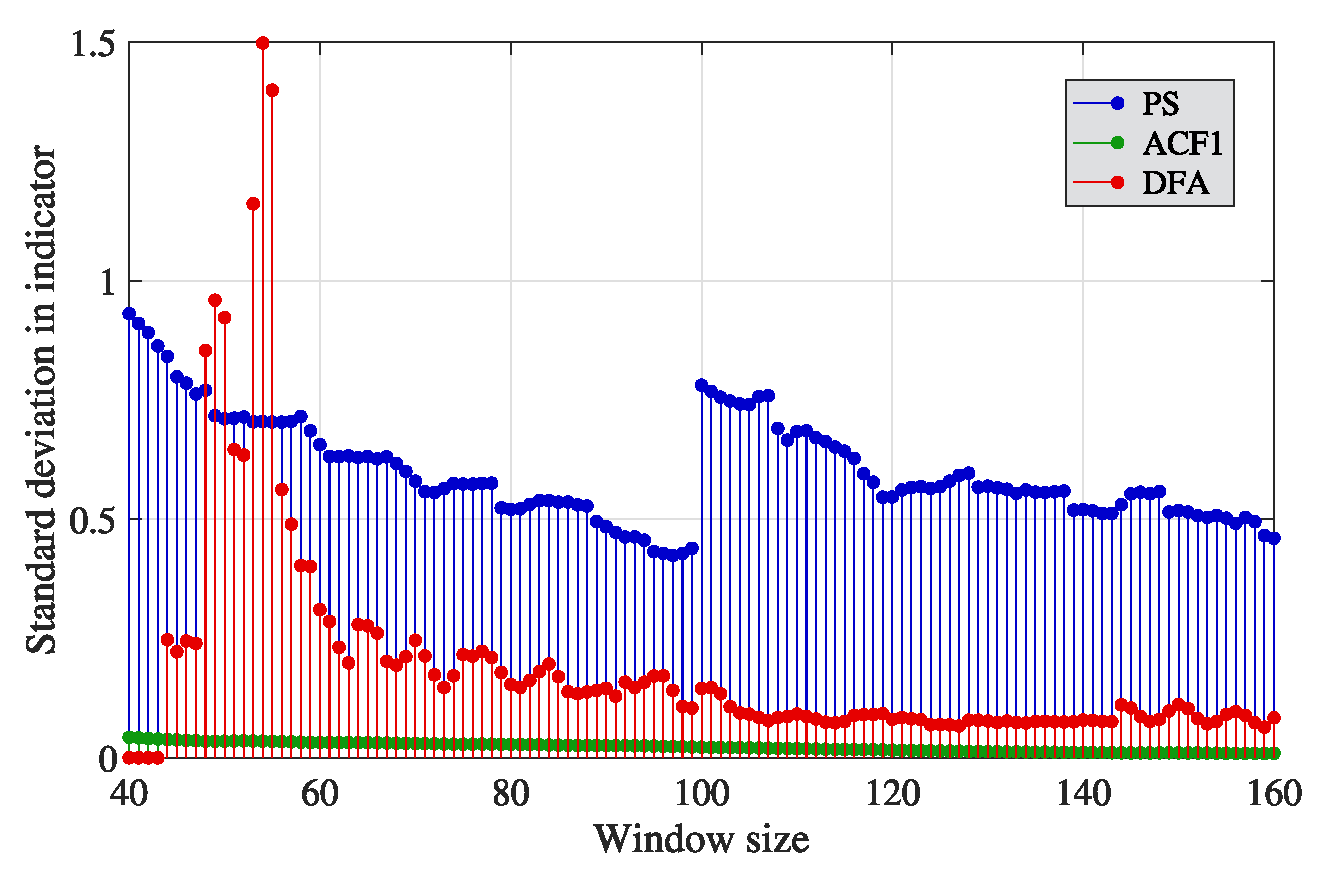
\includegraphics[width = 0.9\textwidth]{stdSensitivity}
	\caption{Sensitivity of the variance in the tipping point indicators to window size. For each window size the standard deviation in the indicator series is calculated for each of the fourteen tropical cyclones and the mean over the fourteen values is plotted.
		\label{fig:TC:stdSensitivity} }
\end{figure}

Figure~\ref{fig:TC:ACF1_sensitivity} is produced by the same method as figure~\ref{fig:TC:PS_sensitivity} but uses the ACF1 indicator. The range of window sizes is also smaller: from 40 to 120, because for sizes over 120 the indicator was consistently above 0.95 and showed no change over the time period. In this case, we notice that the indicator rises, for all window sizes, to a maximum value at around 16 hours before the event, before decreasing sharply. Unfortunately there is something just before -100 hours which causes the ACF1 indicator, particularly with a window size above 60, to be very high –higher than the highest value immediately preceding the cyclone event– which is not visible in the PS and DFA indicators (figures~\ref{fig:TC:PS_sensitivity} and~\ref{fig:TC:DFA_sensitivity}). {\Red{The same pattern is evident in figure~\ref{fig:TC:ACF4_sensitivity} where the ACF4 indicator has been used rather than the ACF1 indicator (that is, the lag-4 autocorrelation function is used in the calculation) since the results presented in figure~\ref{fig:TC:ACF_lags_comp} (see page~\pageref{fig:TC:ACF_lags_comp}) show that a better EWS is visible when lag-4 ACF is used. We note that in this case the value of the indicator is lower (<0.9) over most of the time series and so the increase just before the tipping event is more visible. Additionally, the sharp decrease at the end of the ACF1 indicator signals is not present in the ACF4 indicator signals. }}

\begin{figure}
	\centering
	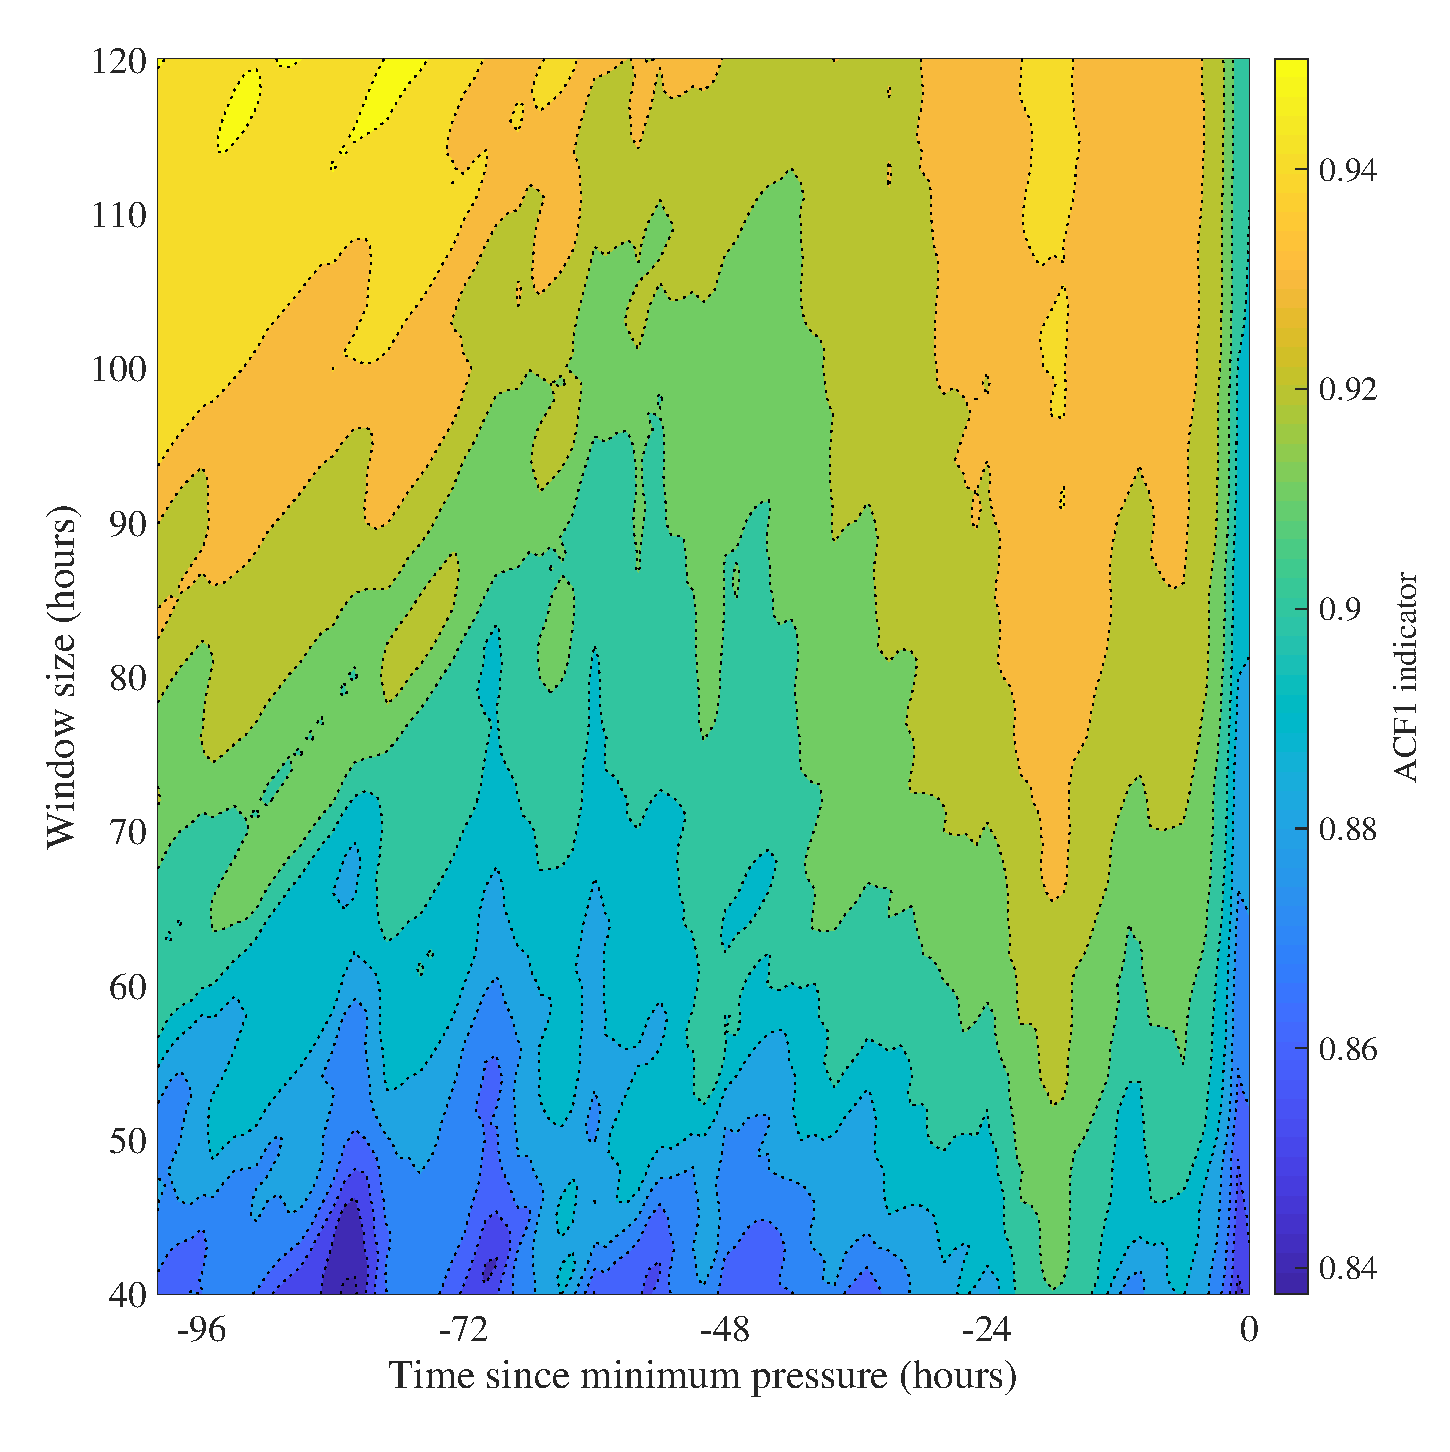
\includegraphics[width = 0.9\textwidth]{ACF1_sensitivity_mean}
	\caption{Mean over 14 tropical cyclones of the ACF1 indicator of the SLP data (see fig. \ref{fig:TC:1DindicatorsSLP}) calculated using window sizes from 40 to 120. The ACF1 indicator appears to rise around 30 hours before the cyclone event in almost all cases. The increase is more pronounced when using a larger window size. \label{fig:TC:ACF1_sensitivity}}
\end{figure}

\begin{figure}
	\centering
	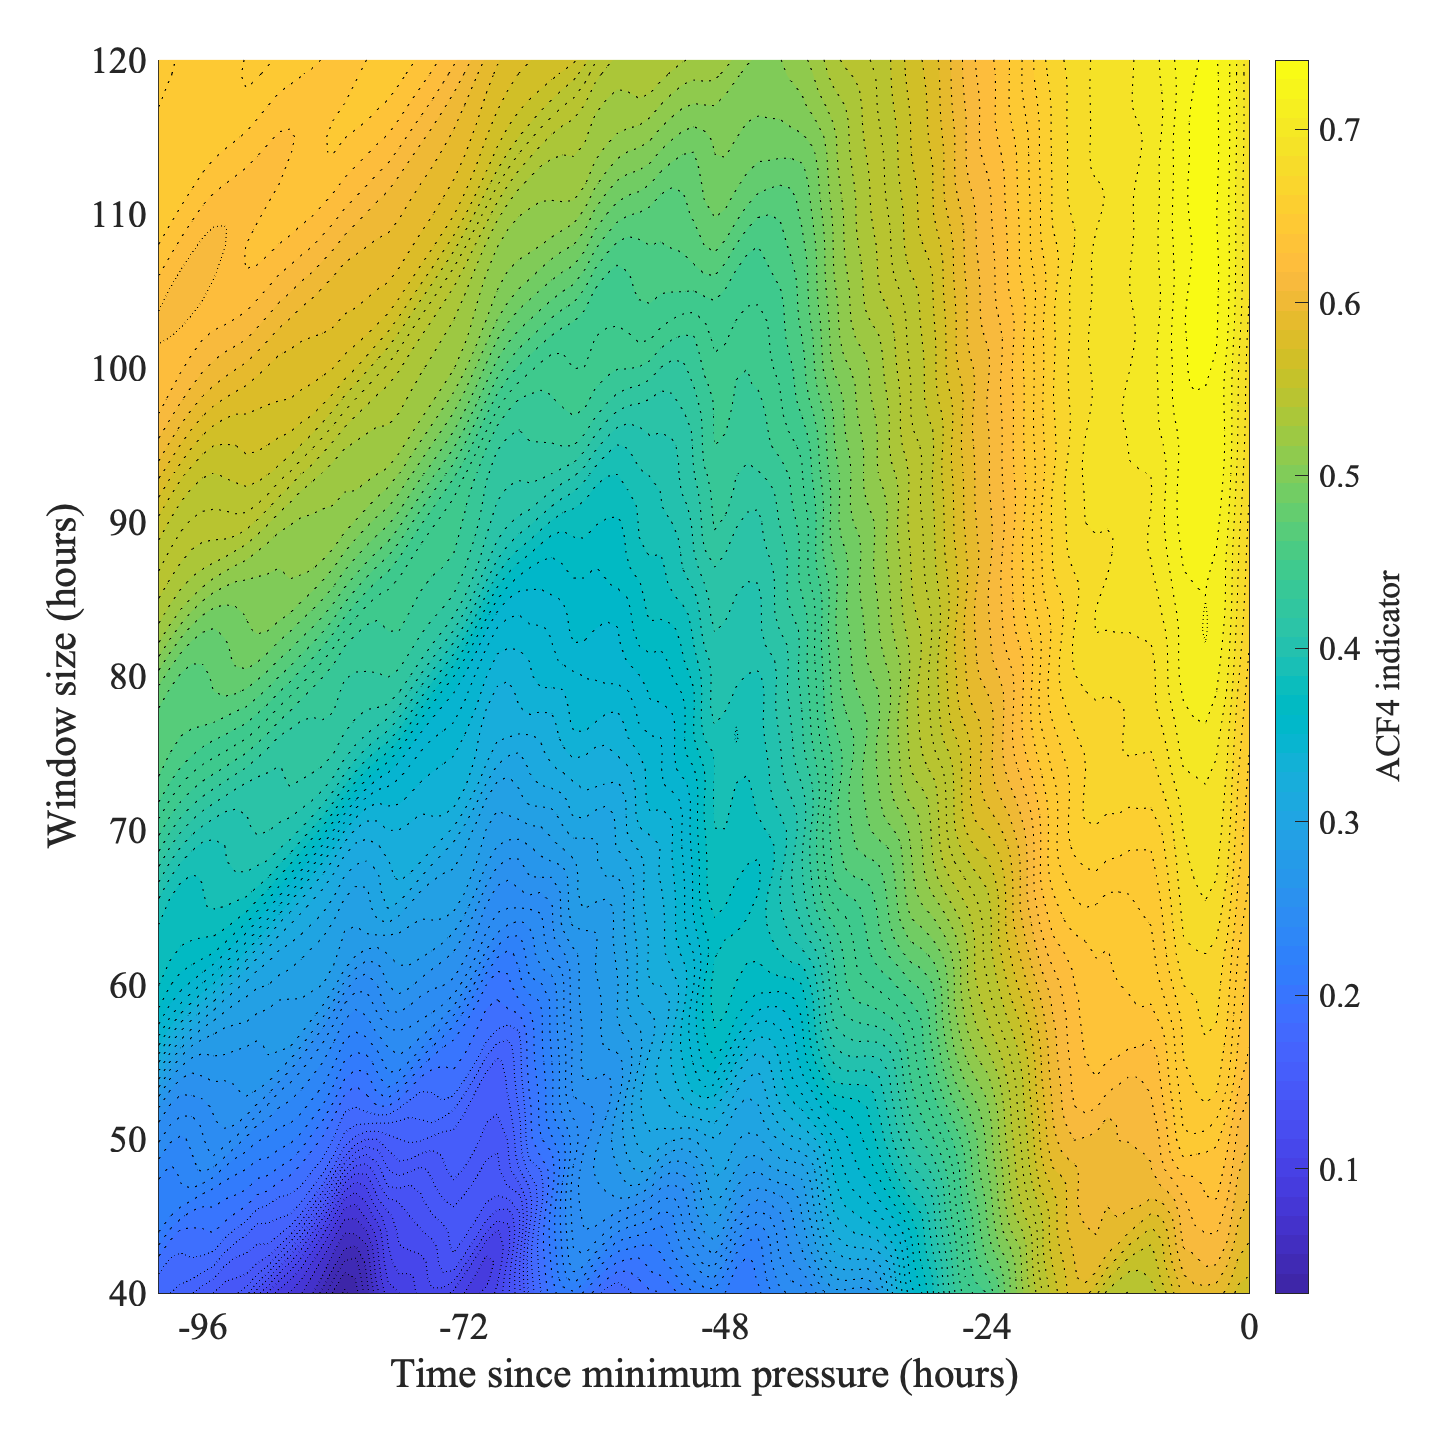
\includegraphics[width = 0.9\textwidth]{ACF4_sensitivity_mean}
	\caption{\Red{Mean over 14 tropical cyclones of the ACF4 indicator (using lag-4 autocorrelation) of the SLP data (see fig. \ref{fig:TC:1DindicatorsSLP}) calculated using window sizes from 40 to 120. The ACF1 indicator appears to rise around 30 hours before the cyclone event in almost all cases. The increase is more pronounced when using a larger window size. We note a similar pattern to the ACF1 indicator in figure~\ref{fig:TC:ACF1_sensitivity}, but the picture is clearer and a clear increase in the indicator can be observed before the tipping event even using very short window sizes.  }}
	\label{fig:TC:ACF4_sensitivity}
\end{figure}

Figure~\ref{fig:TC:DFA_sensitivity} is produced using the DFA indicator, again with a range of window sizes from 40 to 120. The calculation of the DFA scaling exponent is not possible for very short series, depending on how the series is segmented before each segment is detrended by subtracting a polynomial\footnote{In this study we consistently use quadratic detrending to address non-linear effects.}. So as to be able to estimate the scaling exponent, we use eight different segment sizes increasing logarithmically from the smallest to the largest, the smallest being ten points and the largest being $\lfloor N/4\rfloor$ where $N$ is the length of the series. In this way it is always possible to get at least four segments from the series. Using this method it does not make sense to calculate the DFA exponent with a series shorter than 44 points because only one distinct segment size is used, 10, and therefore the relationship between the segment size and the fluctuations coefficient is estimated from a single point.

Table~\ref{tab:TC:DFAsegmentSizes} shows the eight segment sizes used for series lengths 40, 54, 100 and 400. A series length of at least 400 would be ideal, giving a range of segment sizes between 10 and 100 with which to be able to calculate the correlation between the segment size and fluctuations coefficient (see section~\ref{subsec:1D:scaling_exponents:DFA}). With the available data for the sea-level pressure, a window size of 400 points cannot be used. We use a window size of 90 points because there appears to be a slightly stronger early warning signal (an increase in the indicator prior to the event) than with other window sizes. However, the DFA indicator is practically useless when applied to this data.

A series length of 54 is considered in table~\ref{tab:TC:DFAsegmentSizes} because there appears to be interesting oscillating behaviour in figure~\ref{fig:TC:DFA_sensitivity} with a window size of 54. The oscillation has a period of six hours, which suggests a connection with the 12-hour oscillations present in the sea-level pressure data. We also note that there is a qualitative change in the behaviour of the DFA indicator as the window size reaches 80, 91 and (more weakly) 100 points, similar to the change observed in the PS indicator at 100 points (see figure~\ref{fig:TC:PS_sensitivity}). Again, it is not known why this occurs and should be the subject of further investigation. 


\begin{figure}
	\centering
	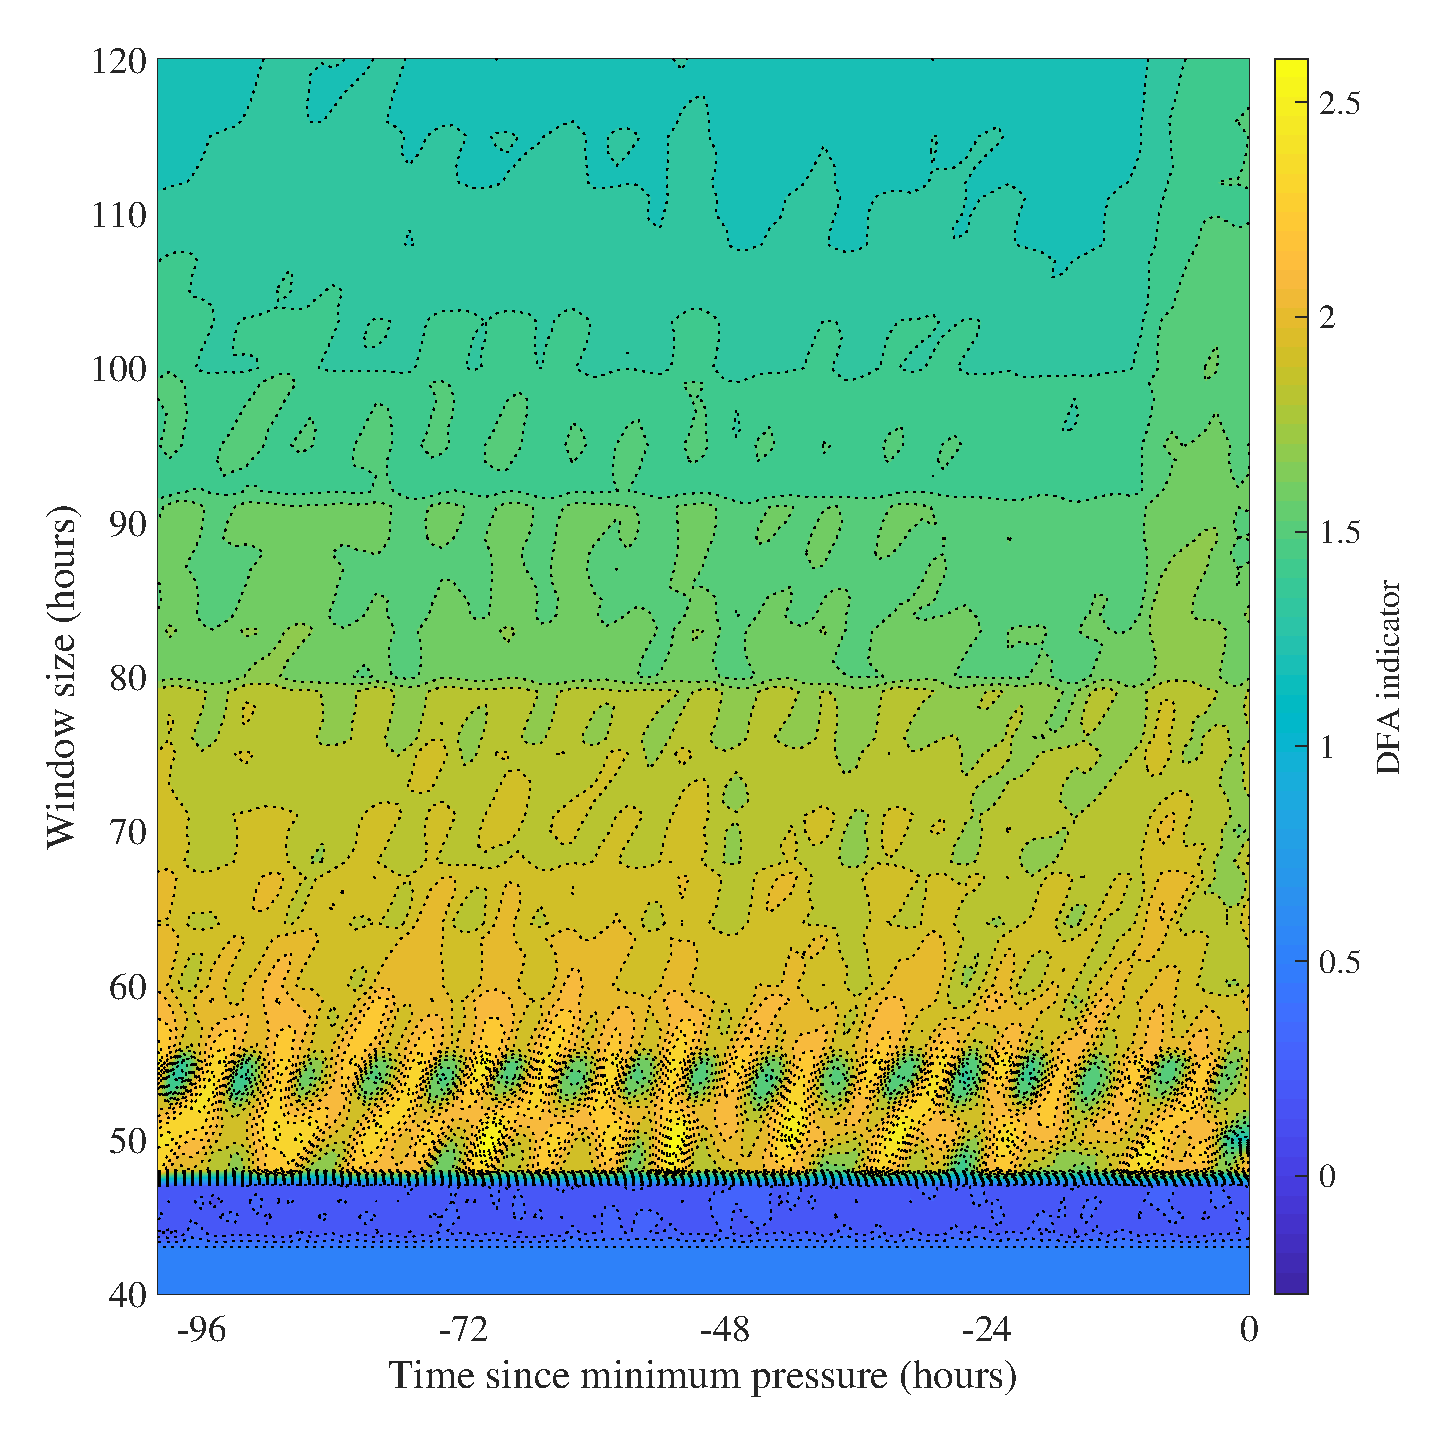
\includegraphics[width = 0.9\textwidth]{DFA_sensitivity_mean}
	\caption{Mean over 14 tropical cyclones of DFA indicator of the SLP data (see fig. \ref{fig:TC:1DindicatorsSLP}) calculated using window sizes from 40 to 120. There is a very small apparent rise in the DFA indicator at -12 hours for window sizes greater than 80 hours. \label{fig:TC:DFA_sensitivity}}
\end{figure}


\begin{table}
	\centering
	\begin{tabular}{c l}
		\hline
		Series length & Segment sizes\\
		\hline
		40  & 10\\
		54  & 10, 11, 12\\
		100 & 10, 11, 12, 14, 16, 19, 21, 25\\
		400 & 10, 13, 19, 26, 37, 51, 71, 100\\
		\hline
	\end{tabular}
	
	\caption{During the calculation of the DFA scaling exponent, a series of length $N$ is segmented eight times, the sizes of the non-overlapping segments increase logarithmically from 10 to $\lfloor N/4\rfloor$. The segment sizes used for four example series lengths are shown. For very short series, fewer than eight different segment sizes may be used.}\label{tab:TC:DFAsegmentSizes}
\end{table}

%\subsection{Investigating autocorrelation with different lags}
%\label{subsec:TC:1D_Lags}
%{\noteRed Maybe? not much to see.}


\section{Application of multi-variable tipping point techniques}
\label{sec:TC:2Dtechniques}

In this section we consider the same fourteen tropical cyclones detailed in table~\ref{tab:TC:14cyclones}. In section~\ref{sec:TC:1Dtechniques}, tipping point indicators were applied to the one-dimensional time series of the sea-level pressure variable at each station. Here, both the wind speed and sea-level pressure are considered together. We first calculate the ACF1, DFA and PS indicator series for the wind speed variable. Using the exact same process by which figure~\ref{fig:TC:1DindicatorsSLP} was produced, showing the indicator series for the sea-level pressure variable, we produce figure~\ref{fig:TC:1DindicatorsWS}, showing the indicator series for the wind speed variable. The same window sizes were used for the ACF1, DFA and PS indicators (90, 90, 102 respectively) as for the sea-level pressure. We note that the mean ACF1 and PS indicators rise with the rising wind speed, and that the DFA indicator performs similarly as in the sea-level pressure case. None of the indicators appear to provide an early warning signal, so we do not expect that combining the wind speed and sea-level pressure variables will yield a signal stronger than already present in the sea-level pressure. However, we proceed to investigate the results of the multi-variable tipping point analysis in comparison to the analysis of the individual variables. 

Throughout this section, including in figure~\ref{fig:TC:1DindicatorsWS}, the time series are aligned so that $t=0$ occurs at the point where the sea-level pressure is minimum, for consistency when comparing to the results in the previous section. This may not be the same point at which wind speed is maximum. {\Red{The results presented in this section have previously been published in \cite{prettyman2019}.}}

\begin{figure}
	\centering
	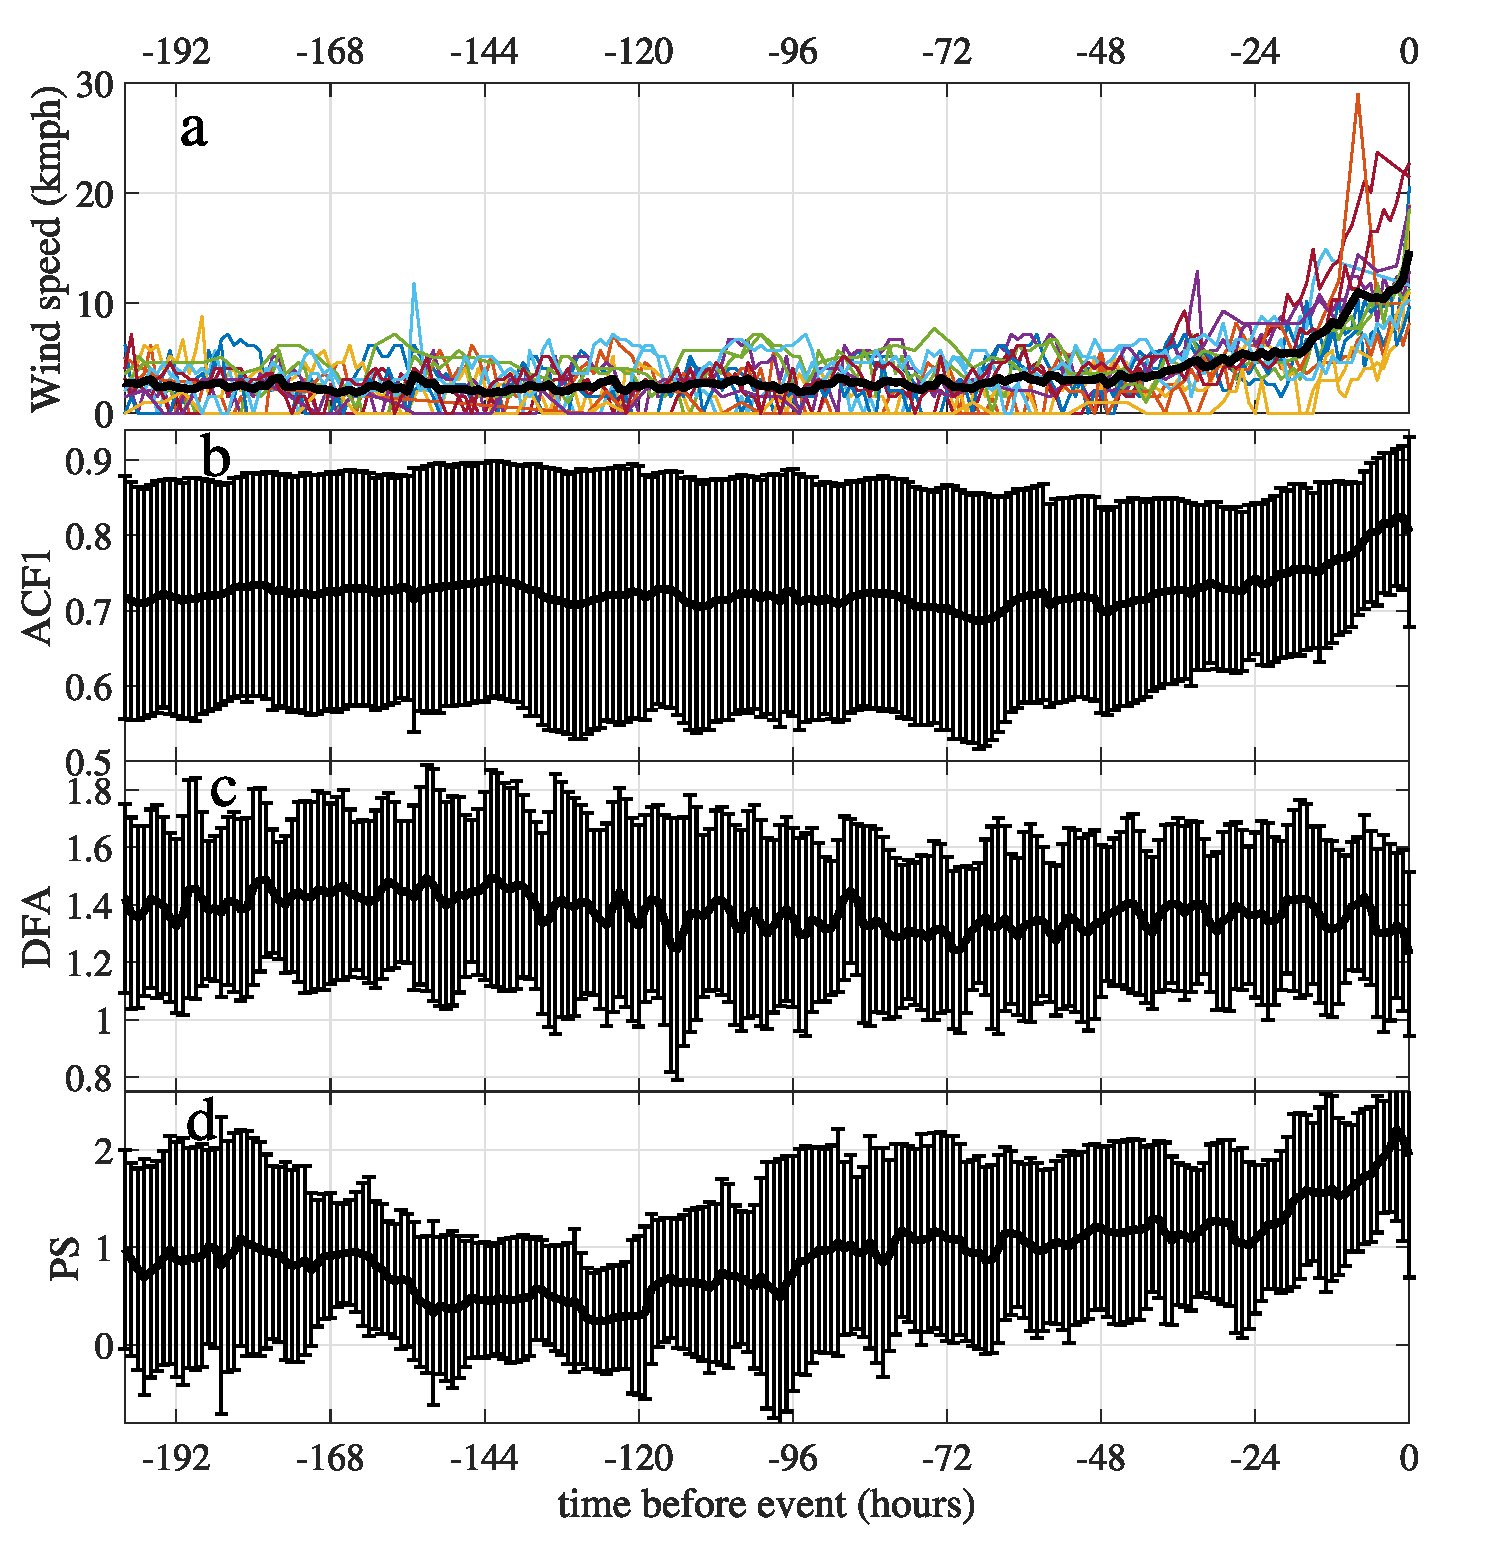
\includegraphics[width = 0.9\textwidth]{indicators14_windspeed}
	\caption{Wind speed data from fourteen tropical cyclones and the mean ACF1, DFA and PS indicators. (a) Wind speed data from the 14 tropical cyclones, mean shown in black. (b,c,d) The mean ACF1, DFA and PS indicators, with error bars of 1 standard deviation. \label{fig:TC:1DindicatorsWS}}
\end{figure}

\subsection{Method}
\label{subsec:TC:2Dmethod}

Having considered the sea-level pressure and wind speed variables separately (figures~\ref{fig:TC:1DindicatorsSLP} and~\ref{fig:TC:1DindicatorsWS}) we now combine the two variables so that more data is available from which to produce a single tipping point indicator series. We use the the methods introduced in sections~\ref{sec:2D:Williamson} and~\ref{sec:2D:EOF}, that is, the analysis of the eigenvalues of the Jacobian matrix of a linearised system, and the use of EOFs to reduce the dimension before applying the one-dimensional indicator techniques.  

\subsubsection{Jacobian eigenvalues analysis}
For the Jacobian eigenvalues analysis we repeat the method described in section~\ref{sec:2D:Williamson} using a window size of 102 points in order to provide a comparison with the PS indicator applied to the one-dimensional sea-level pressure time series, for which this window size is used. In section~\ref{subsec:TC:2D_SA} we will perform a sensitivity analysis to determine whether a different window size is preferable. Besides the window size, it is necessary to choose whether to study the real part, the imaginary part, or the complete complex eigenvalue. Since we do not know in advance the nature of the tipping, we record both the real and imaginary parts. Thus, in a sliding window of 102 points, the Jacobian matrix of the linearised system is estimated from the two system variables (sea-level pressure and wind speed) and the principal eigenvalue is recorded. The method of approximating Jacobian eigenvalues has previously been applied to dynamical systems where the governing equations and the type of bifurcation are known \citep{williamson2015}, and so we know in advance what type of signal we should expect, such as with the example of the Van der Pol oscillator in the previous chapter (figure~\ref{fig:2D:vdpIndicators}). However, we have noted that the method was intentioned as a two-dimensional analogue to the lag-1 autocorrelation, so it is reasonable to apply it to systems in which the one-dimensional ACF1 indicator, and the related PS and DFA indicators, increase prior to a tipping point. We are particularly interested to note the extent to which this indicator is an improvement, if at all, over simply considering the one-dimensional indicators individually, and whether any additional artefacts arise as a consequence of considering the two variables together.

\subsubsection{Dimension reduction using EOFs}
The other technique we use here is to first obtain the the leading EOF score of the two time series (sea-level pressure and wind speed) in order to reduce the dimension to one. The time series in both variables are first mean-centred, as per the EOF method, and also normalised in order to non-dimensionalise. We are then able to apply the one-dimensional EWS techniques, the ACF1 and PS indicators, and take the mean over all cyclones. We use a window size of 102 for the PS indicator and 90 for the ACF1 indicator, since these were found to be useful when considering the sea-level pressure alone in the previous section.

As noted in section~\ref{subsec:2D:EOF:movingEOF}, there are three available approaches to obtaining the principal EOF score, that is, there are three approaches to obtaining the vector onto which we project the two-variable series. The vector is the principal eigenvector of the covariance matrix of two time series, we may use either
\begin{enumerate}
	\item the entire available time series (global projection), or
	\item only the segment of the time series in each window (windowed projection), or
	\item the entire available time series \emph{up to} the end of the current window (moving projection).
\end{enumerate}
The first option in this case implies using the part of the time series which lies in the "future" of the current window. This is not comparable to practical prediction problems and so we avoid it here. It is also not sensible to obtain the projection vector using the part of the time series which includes the tipping point when considering the rest of the series, because the dynamics are not representative. 

The second and third options are distinguished in section~\ref{subsec:2D:MethodsApplied:Hopf_movingEOF}. The windowed projection most accurately captures the maximum variance in each window, but may be unsuitable if the principal EOF eigenvector is highly variable due to noise. In this system we want to avoid considering signals from meteorological events prior to the tropical cyclone being studied and want to, as much as possible, consider a relatively stationary system prior to the tipping event. To this end, we generally truncate the time series at around 300 hours before the tipping point and so the total length of the series is not much longer than the window size used in the indicator calculation (approximately 100 hours). Therefore, the difference between using the windowed or moving projection will be negligible. Throughout this section, we use the windowed projection.

Since the two variables have different units, it is not meaningful to consider them together without first non-dimensionalising. To satisfy this requirement, as part of the EOF technique, each time series is mean-centred and normalised by its own standard deviation. In section~\ref{subsec:TC:2D_SA} we explain the investigation into the effect of weighting the two variables differently, as a result of which we choose to weight the sea-level pressure and wind speed variables in the ration $40:60$ when using the ACF1 indicator, and to weight the variables equally when using the PS indicator.

\subsection{Results}
\label{subsec:TC:2Dresults}

The Jacobian eigenvalue analysis is performed separately for each cyclone and both the real and imaginary parts of the principal eigenvalue are recorded. The mean of the fourteen resulting indicator series is shown in figure~\ref{fig:TC:indicators_WLandEOF}a,b, with error bars of one standard deviation over the fourteen indicators. We note that there is a slight increasing trend in the real part of the eigenvalue starting at around 48 hours before the minimum pressure, similarly to the PS indicator applied to the sea-level pressure series (figure~\ref{fig:TC:1DindicatorsSLP}). The imaginary part also exhibits a spike as the event occurs. 

The results of applying the ACF1 and PS indicators to the windowed EOF projection are shown in figure~\ref{fig:TC:indicators_WLandEOF}c,d. We note that the rise in the ACF1 indicator is more noticeable than when using only the sea-level pressure (figure~\ref{fig:TC:1DindicatorsSLP}b), but is not so noticeable as when using only the wind speed (figure~\ref{fig:TC:1DindicatorsWS}b). The combination of the two variables using EOF has given an indicator series which appears to be somewhere between the two separate indicator series, although it is not equivalent to simply taking the mean of the two. The PS indicator series is more similar to the PS indicator series using only sea-level pressure (figure~\ref{fig:TC:1DindicatorsSLP}d). We quantify the gradient of the indicator by evaluating the Mann-Kendall coefficient of the mean indicator series in the 30-hour window before time zero, using the equation
\begin{equation}
	c(X) = \frac{2}{N(N-1)}\sum_{i=1}^{N-1}\sum_{j=i+1}^{N}\text{sign}(X_j-X_i)\,,
	\label{eqn:TC:MannKendall}
\end{equation} 
where $X$ is the time series of the indicator. The result is summarised in table~\ref{tab:TC:EOFresults}.

	\begin{table}
		\centering
		\begin{tabular}{l c c}
			\hline
			& \multicolumn{2}{c}{Indicator} \\
			\cline{2-3}
			Data & ACF1 & PS\\
			\hline
			Sea-level pressure & -0.20 & 0.79 \\
			Wind speed & 0.91 & 0.70 \\
			EOF & 0.45 & 0.72\\
			\hline
		\end{tabular}
		
		\caption{Comparison of the Mann-Kendall coefficient of the ACF1 and PS indicators of the time series data in a 30-hour window before the tropical cyclone event. We compare sea-level pressure and wind speed data alone (as presented in figures~\ref{fig:TC:1DindicatorsSLP} and~\ref{fig:TC:1DindicatorsWS}) to the EOF score of the two series (figure~\ref{fig:TC:indicators_WLandEOF}c,d). In the case of each indicator, the EOF result has a gradient somewhere between the two considered alone.}\label{tab:TC:EOFresults}
	\end{table}

\begin{figure}
	\centering
	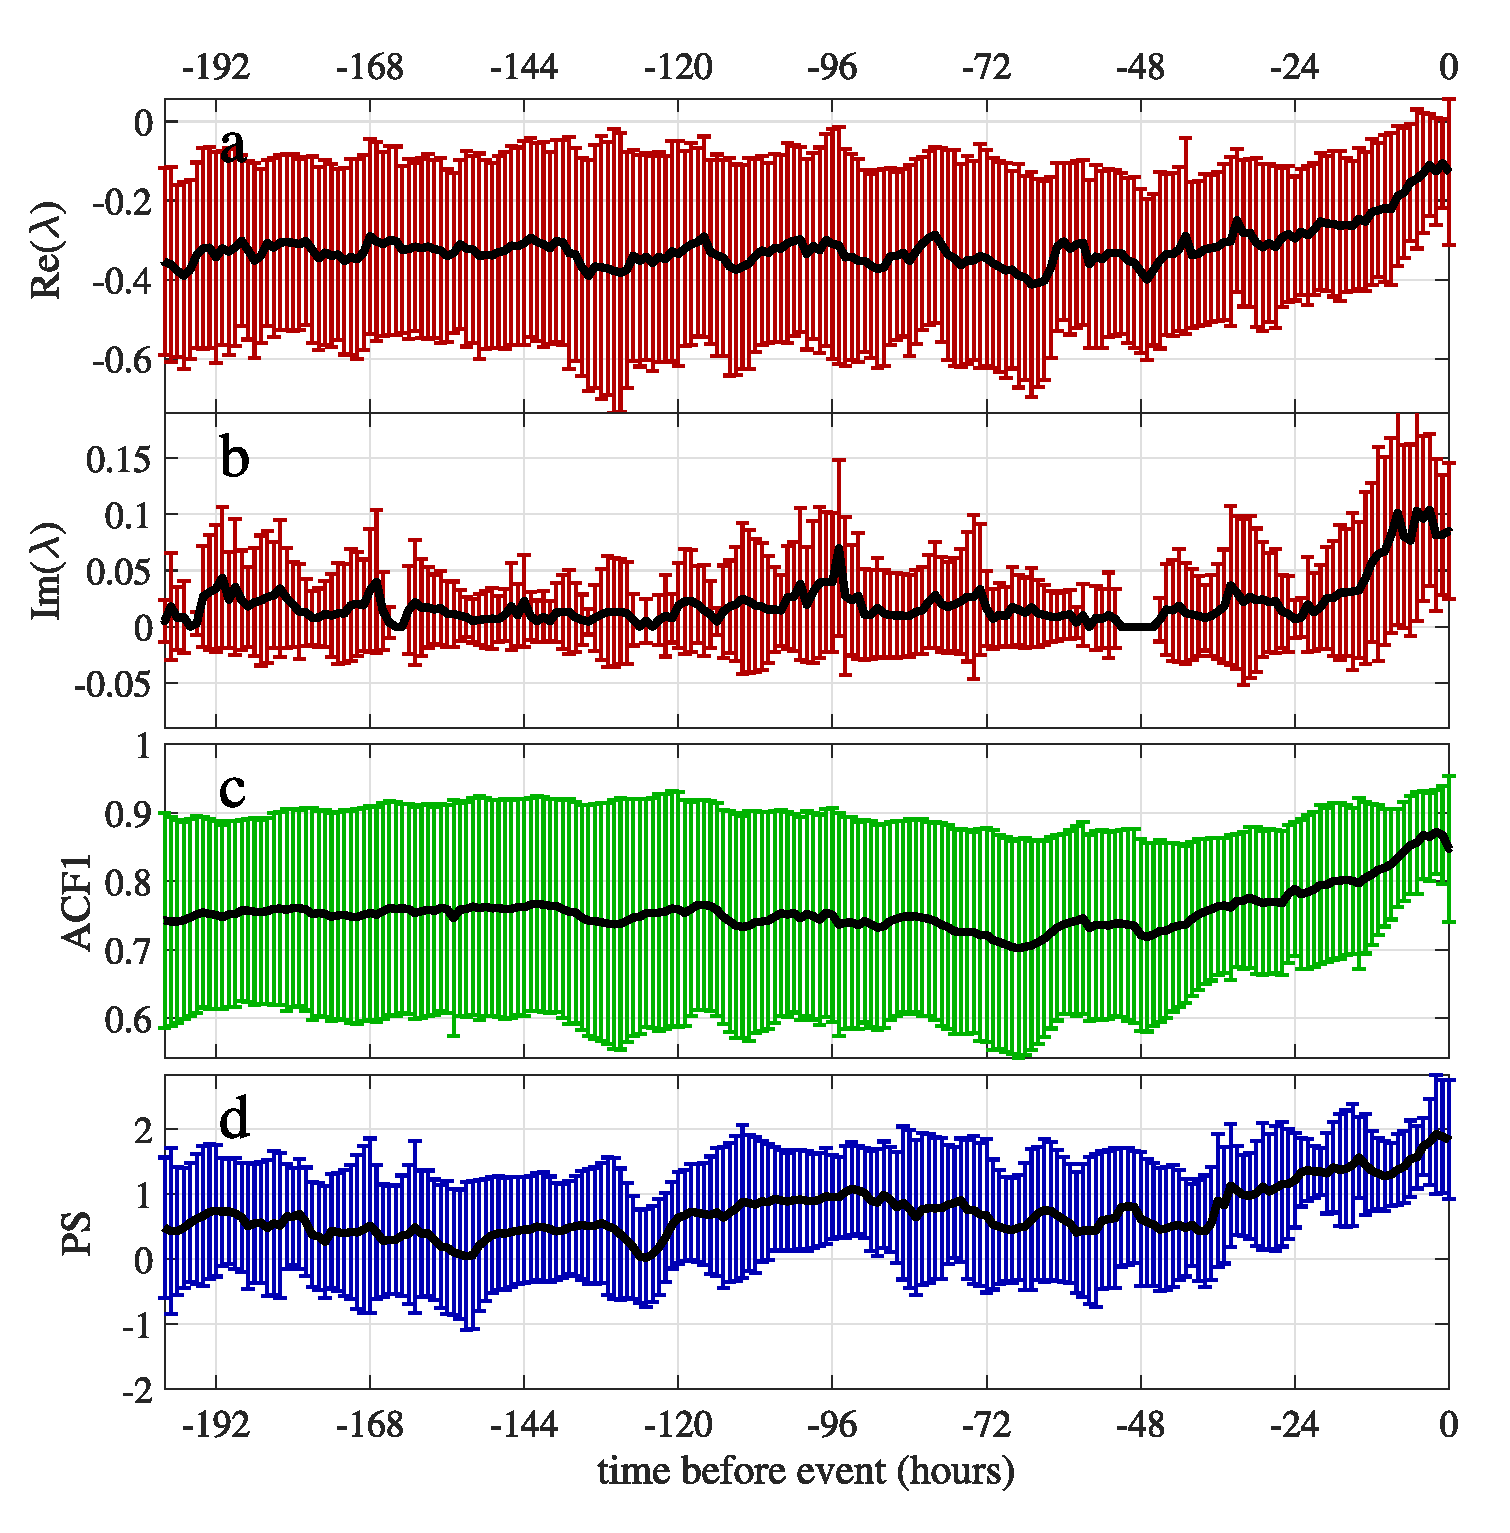
\includegraphics[width = 0.9\textwidth]{indicators_WLandEOF} \caption{\label{fig:TC:indicators_WLandEOF} Multivariate indicator methods applied to sea-level pressure and wind speed data in fourteen tropical cyclones. Mean value shown in black with error bars of one standard deviation over the fourteen series. Panels \textbf{a} and \textbf{b}: the real and imaginary parts of the principal Jacobian eigenvalue calculated in a sliding window of 90 hours. Panels \textbf{c} and \textbf{d}: the ACF1 and PS indicators calculated for the windowed EOF projection using window sizes 90 and 102 hours respectively. For the ACF1 indicator, the sea-level pressure and wind speed variables are weighted $40:60$.}
\end{figure}


\subsection{Weighting sensitivity in EOF techniques}
\label{subsec:TC:2D_SA}

The Jacobian eigenvalues technique takes into account only the covariance between the two variables and is not sensitive to the relative weights of the variables. That is, if the data in one column were changed to different units resulting in values many times larger, the eigenvalues (but not the eigenvectors, which are not studied) would not change. The calculation of EOFs, however, is sensitive to different weighting schemes. By multiplying each variable (each column of the data matrix) by different scalar values, we are able to assign greater or lesser importance to each variable. 

We are therefore able, by visualising the indicator series for a variety of different weighting schemes, to select an optimum weighting in each case. For the data matrix $X$, where the columns of $X$ are the time series variables, we instead use the weighted matrix 
	\begin{equation}
		X_{w} = XW,
	\end{equation}
where, in our case,
	\begin{equation}
		W = \begin{bmatrix}
		p & 0\\
		0 & 1-p
		\end{bmatrix}~,~~~~~p\in [0,1].
	\end{equation}
For $p=0$ the first column of $X$, in our case the sea-level pressure variable, is given no weight and the indicator series is identical to the one-dimensional indicator applied to wind speed alone. Conversely, when $p=1$, only the sea-level pressure is considered. 

\begin{figure}
	\centering
	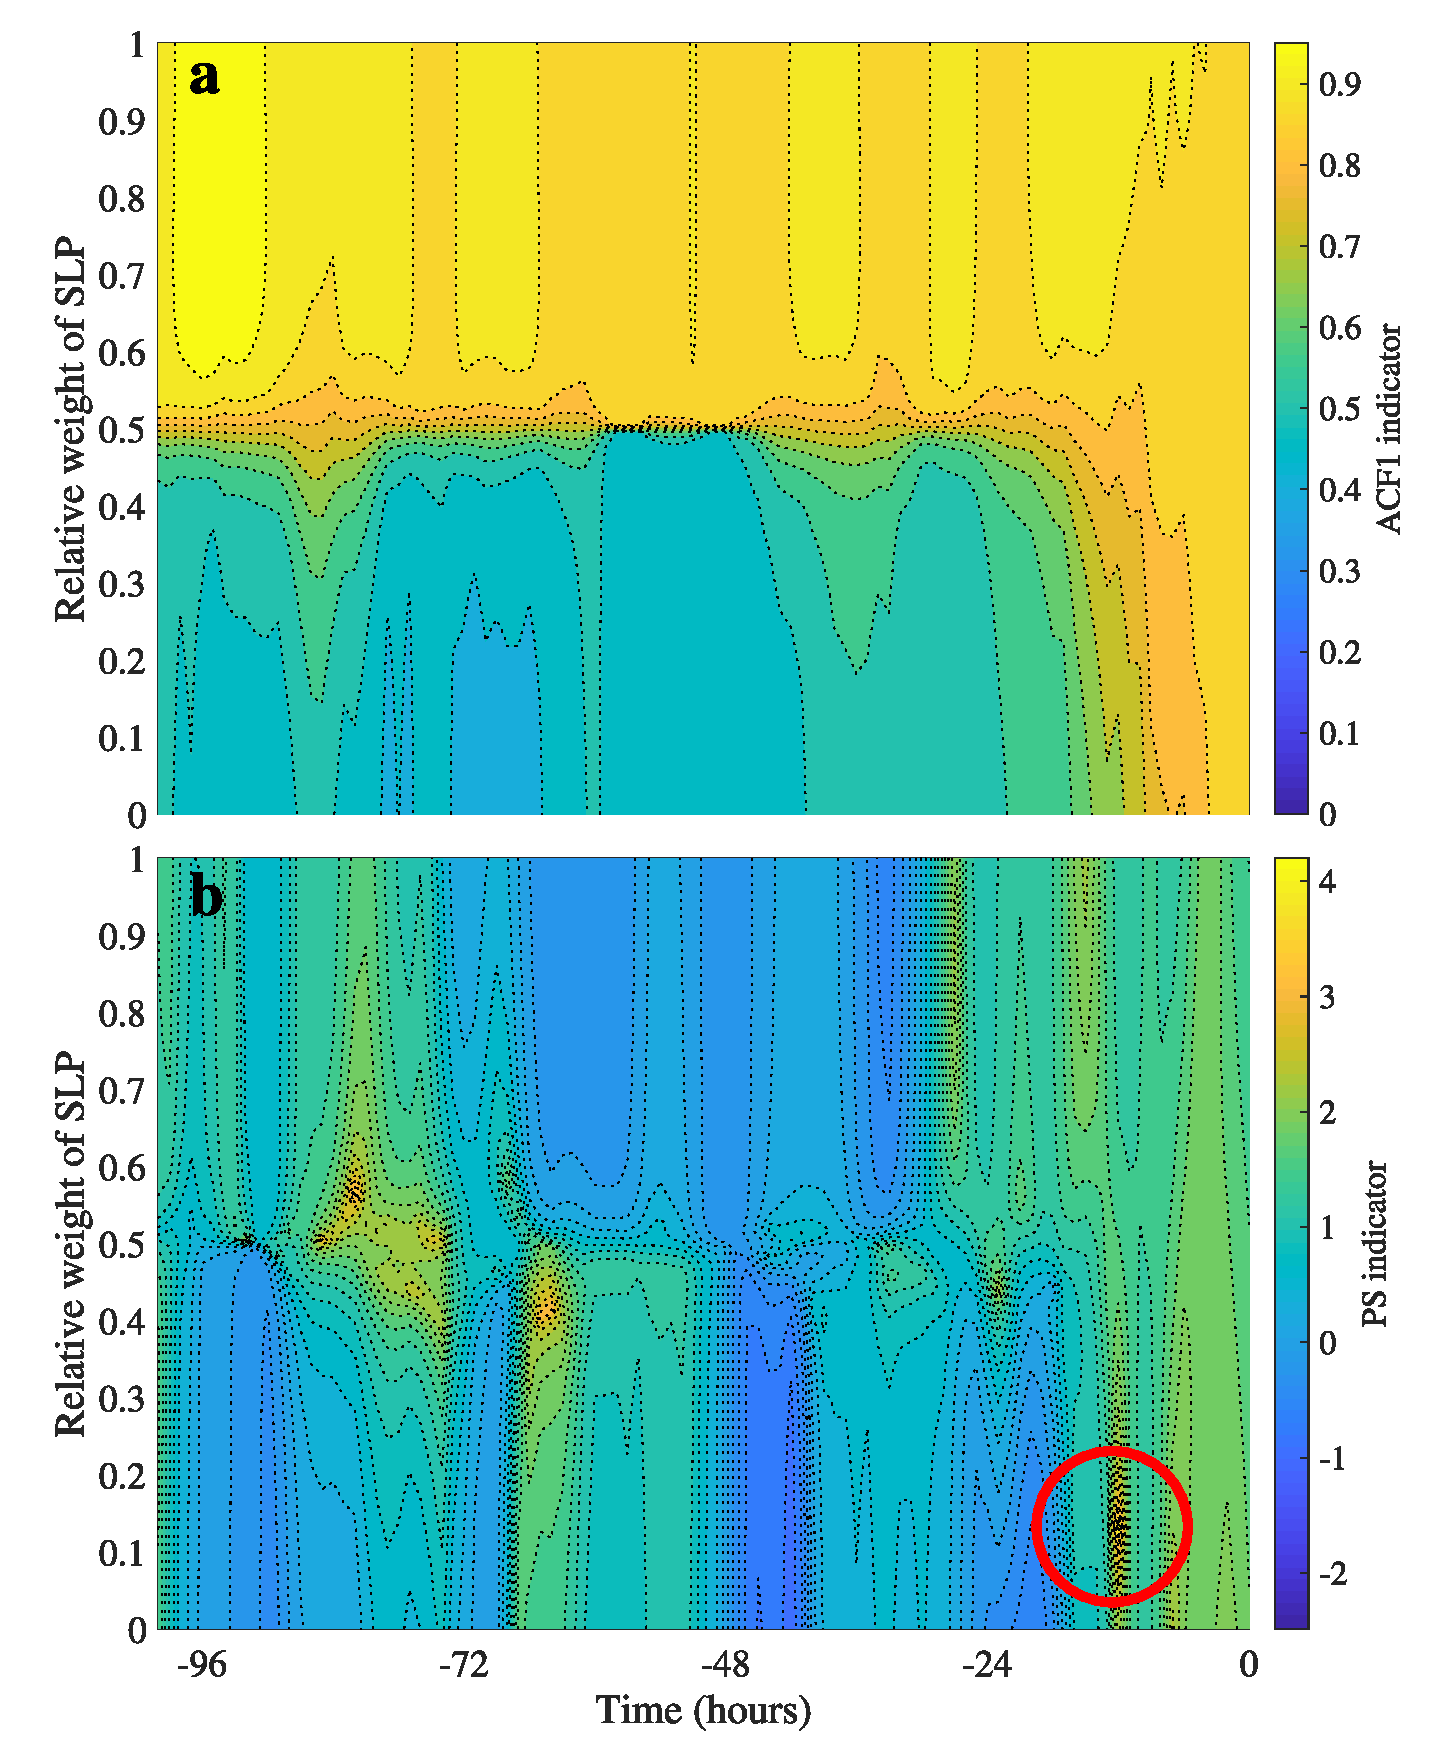
\includegraphics[width=0.9\textwidth]{weightsensitivity_both}\caption{Sensitivity of the ACF1 and PS indicators to different EOF weighting schemes. The widowed EOF projection is found for a range of SLP weighting values from $p=0$ (only wind speed considered) to $p=1$ (only SLP considered) and the ACF1 and PS indicators are calculated (panels \textbf{a} and \textbf{b} respectively). A non-periodic spike in the PS indicator is circled in red. \label{fig:TC:weightSensitivity} }
\end{figure}

The EOF projection is found for a range of values from $p=0$ to $p=1$ and the PS and ACF1 indicators are calculated. The results for the ACF1 indicator and the PS indicator are both shown as contour plots in figure~\ref{fig:TC:weightSensitivity}. We note that, when using the ACF1 indicator, there is a clear difference between $p<0.5$ and $p>0.5$. Weighting the sea-level pressure variable at $0.4$ is effectively equivalent to weighting it zero. Likewise, weighting the SLP variable at $0.6$ is effectively equivalent to weighting it $1$. When SLP is weighted more heavily than wind speed ($p>0.5$) the ACF1 indicator is consistently high and does not provide an EWS, which is already apparent from the ACF1 indicator applied to SLP alone (see figure~\ref{fig:TC:1DindicatorsSLP}b). Using $p<0.5$ there is an increase in the indicator prior to the event, as in figure~\ref{fig:TC:1DindicatorsWS}b, and this rise appears earlier as the relative weight of the SLP variable increases, up to the complete qualitative change at $p=0.5$. It appears that choosing a value $p=0.4$ would provide the best EWS in this case. 

For the PS indicator, the picture is more similar for different weighting schemes. The contour plot is complicated by a few unexplained spikes with much higher indicator values than the surrounding points. For example, for the specific weighting $p=0.15$ there occurs a non-periodic spike at -12 hours where the PS indicator is greater than $3$, this spike is circled in red in figure~\ref{fig:TC:weightSensitivity}. It is possible that this approach could be used to determine specific weightings to avoid, based on the presence of spikes, but this would not be practical without prior knowledge of the spikes' distribution.


\section[Spatially separated data]{Early warning signals for tropical cyclones using spatially distributed data}
\label{sec:TC:field_data}

Here we make an attempt to use the one-dimensional EWS indicators applied to multiple time series data distributed over a geographic area. We investigate the spatial variation in the indicator series, potentially with a view towards detecting a spatial pattern which may provide a warning of the arrival of the tropical cyclone. {\Red{The results presented in this section have previously been published in \cite{prettyman2019}.}}


\subsection{Method}
\label{subsec:TC:fieldmethod}

For this analysis nine separate tropical cyclone events were selected (see section~\ref{subsec:TC:data:HadISD}) which are described in table~\ref{tab:TC:9hurricanes}. {\Red{These events were selected due to an availability of data at several stations within 200~km of the landfall location of the hurricane, which gives between $21$ and $48$ stations depending on the hurricane (see column ``\# stations'' in table~\ref{tab:TC:9hurricanes}, page~\pageref{tab:TC:9hurricanes}).}} The sea-level pressure data were obtained from each station within this radius in a period of twenty days before landfall, and stations were disregarded where more than ten points were missing during this period. The data from the remaining stations were linearly interpolated onto the entire one-hourly time series.

For each of the nine hurricanes, we take the sea level pressure data from all available stations in the region supplied by the HadISD 2017 dataset. We then calculate the PS indicator series for each pressure dataset and asses the slope of that indicator series, using the Mann-Kendall coefficient (see equation~\ref{eqn:TC:MannKendall}), in a window of approximately 30 hours before the hurricane enters the region. If the behaviour here is similar to the behaviour of the mean of the PS indicator applied to the individual sea level pressure series (figure~\ref{fig:TC:1DindicatorsSLP}d), we would expect that an upward trend in the indicator (i.e. a high positive value of the Mann-Kendall coefficient) will be detectable for each location within 30-hours travelling time of the hurricane. We expect that the slope of the PS indicator series would be high at points where the hurricane is very close and lower at points further from the point where the hurricane enters the region. 

The window size used in the calculation of the PS indicator series, and the length of the window in which the Mann-Kendall coefficient is evaluated, are determined for each hurricane through a sensitivity analysis similarly to the process described in section~\ref{subsec:TC:1D_SA}, which is presented in figure~\ref{fig:TC:3by3_sensitivity}. In these contour plots, the mean is not taken over the indicator series for all tropical cyclones, as in section~\ref{subsec:TC:1D_SA}, but rather an individual contour plot is presented for each cyclone in which the mean is taken over all the stations in that region. We see that there is again a significant qualitative change as the window size increases over 100 hours. We note that the increase in the indicator is usually seen in a 30-50 hour window before the event, which is consistent with our expectations based on previous analysis.

As a result of the sensitivity analysis in figure~\ref{fig:TC:3by3_sensitivity} we take the decision to measure the Mann-Kendall coefficient of the indicator series (for the time series at each spatial location, separately) in a 30-50 hour window before a time $T_{\text{entry}}$, which is when the cyclone enters the region under study: that is the time at which the minimum pressure is attained at the first spatial location on the cyclone's path. We expect to see a high coefficient value (i.e. a large increase in the indicator) at locations close to the entry point.
	\begin{figure}
		\centering
		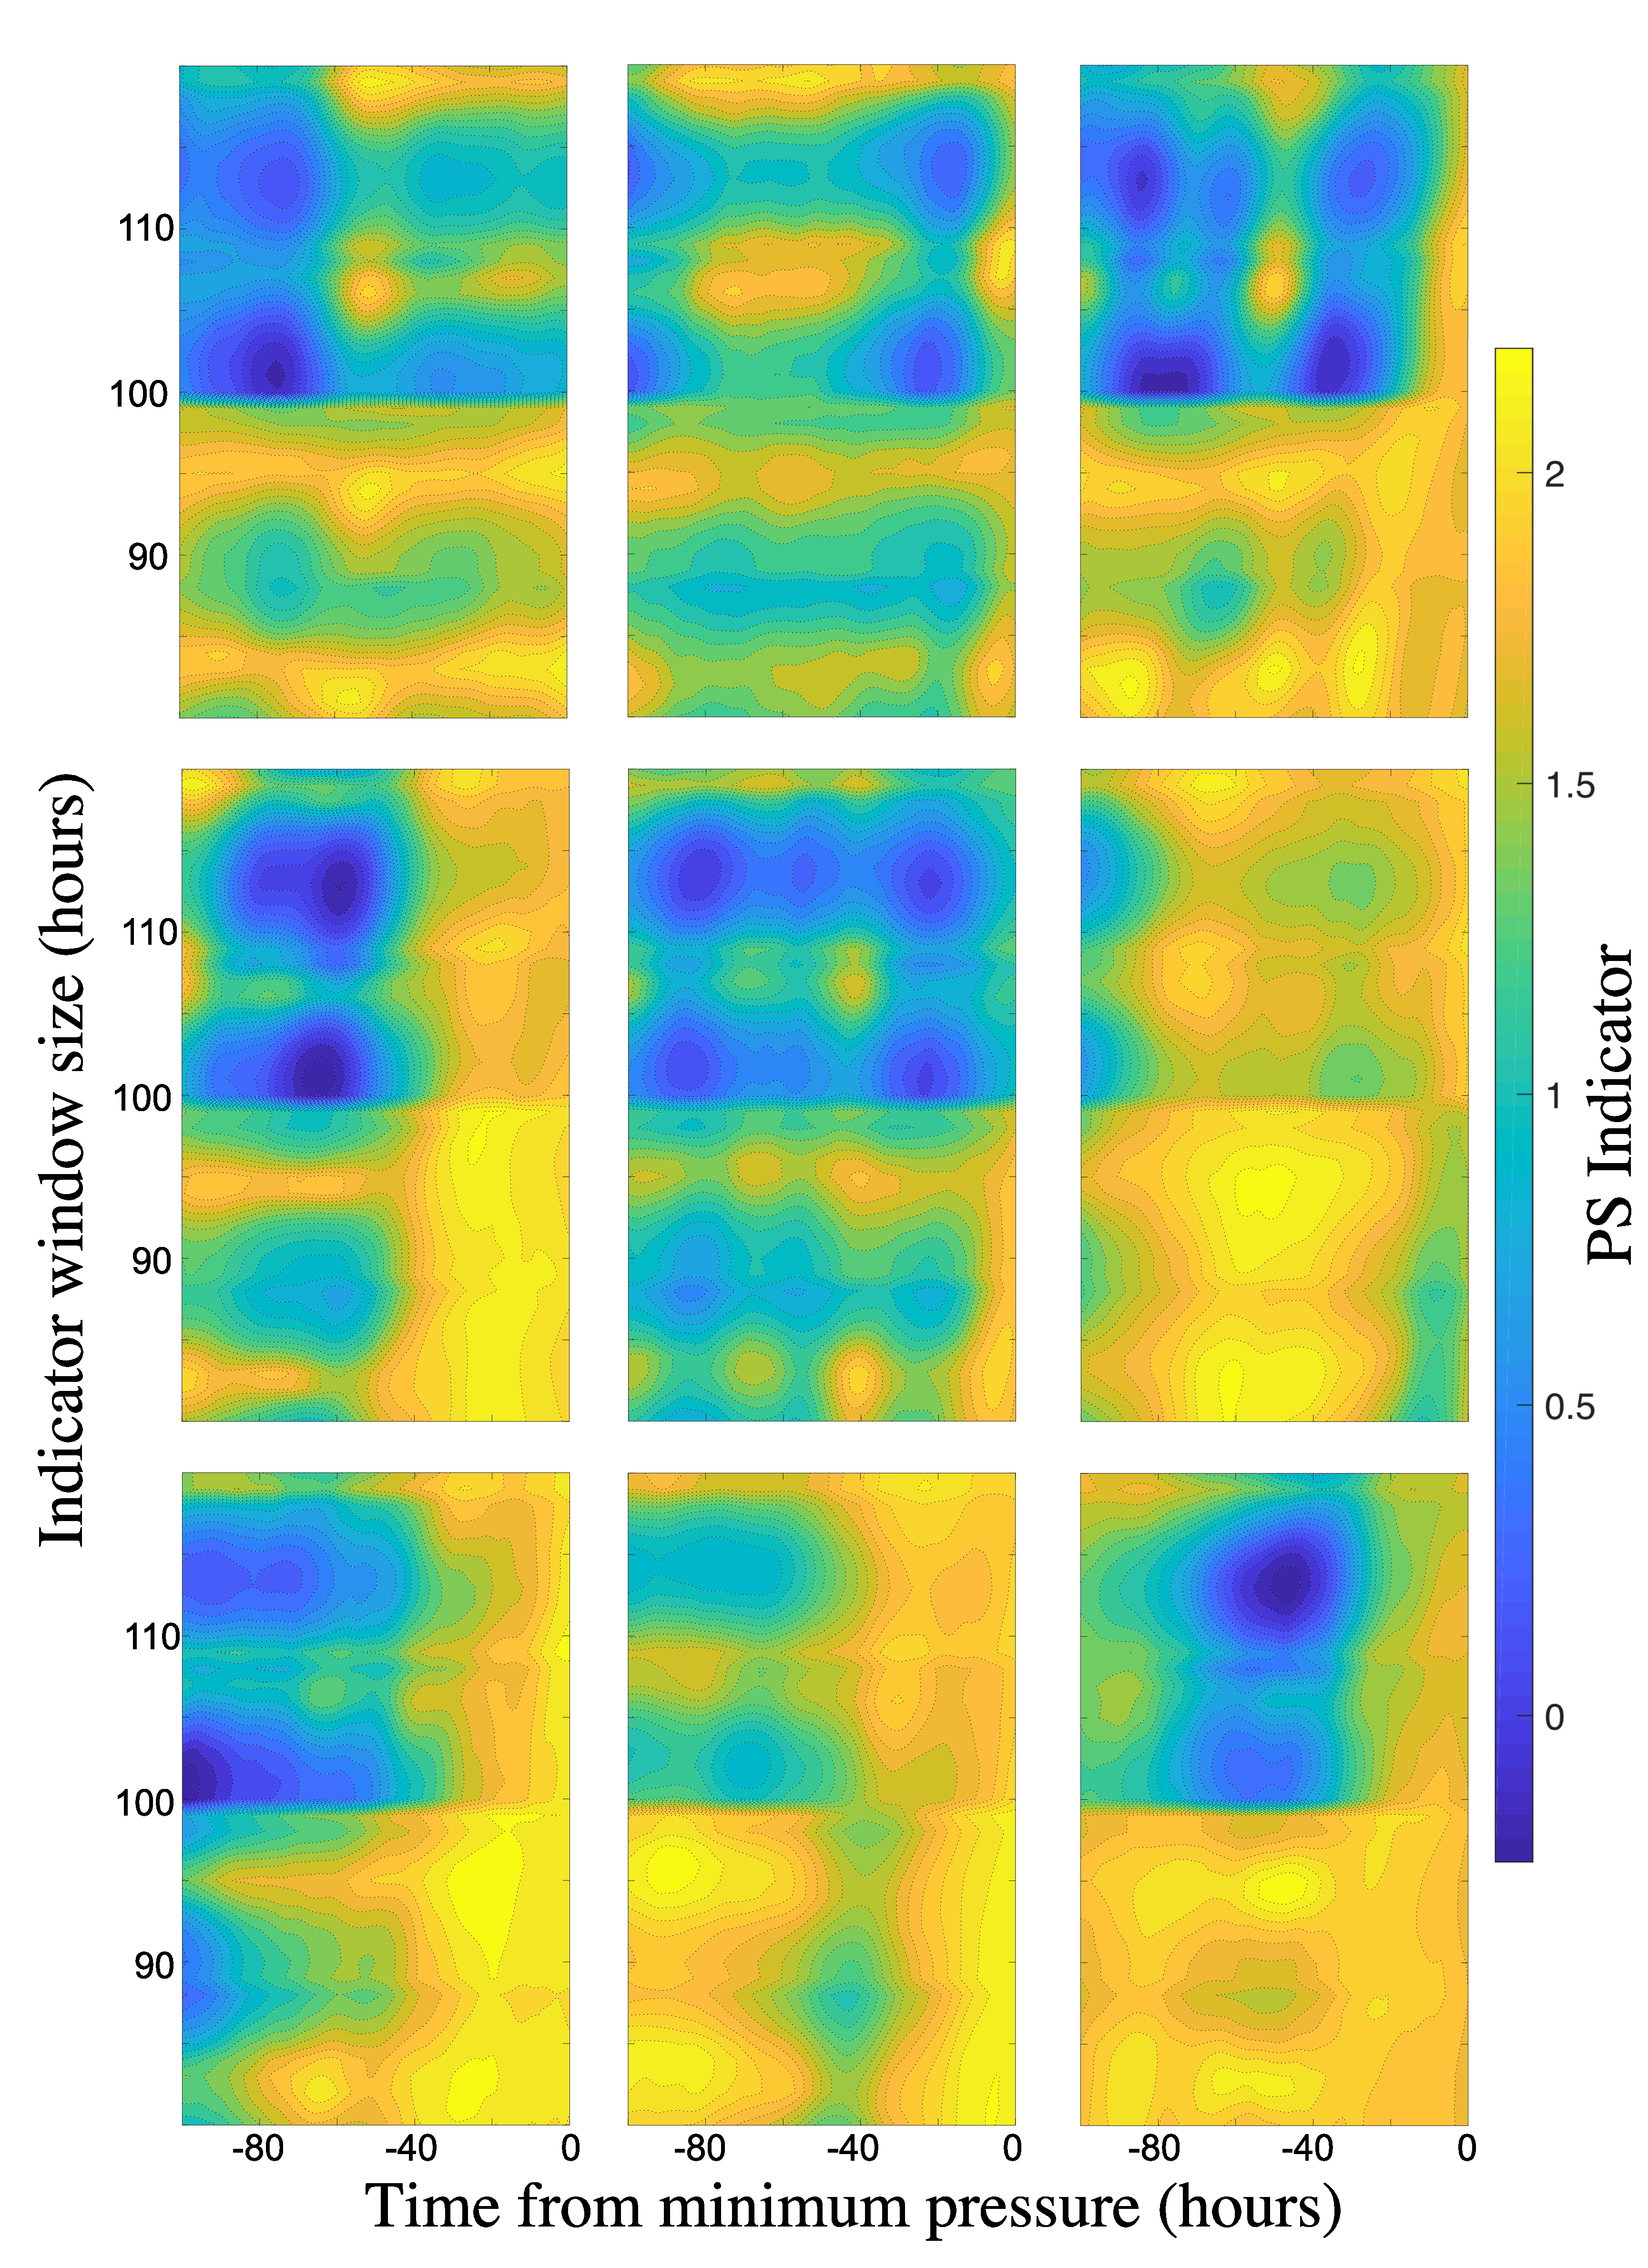
\includegraphics[width = 0.9\textwidth]{Sensitivity3x3}
		\caption{\label{fig:TC:3by3_sensitivity} Contour plots showing the sensitivity of the PS indicator to the window size. Reading left to right the plots show the results for: Andrew (Florida); Andrew (Louisiana); Katrina; Wilma; Gustav; Matthew; Harvey; Irma; Nate. In each case, for each window size, the PS indicator is calculated for the sea-level pressure time series given at each station in the landfall region and the mean taken over all of these stations.}
	\end{figure}
Also, according to the sensitivity analysis, we note that the PS indicator is most useful when using a window size which is an odd multiple of six, consistent with the result of the previous sensitivity analysis in section~\ref{subsec:TC:1D_SA}. This is likely due to the 12-hour tidal oscillations in the data. For each cyclone we have chosen an indicator window size of either 90 or 102 points.

\subsection{Results}
\label{subsec:TC:fieldresults}

\begin{figure}
	\centering
	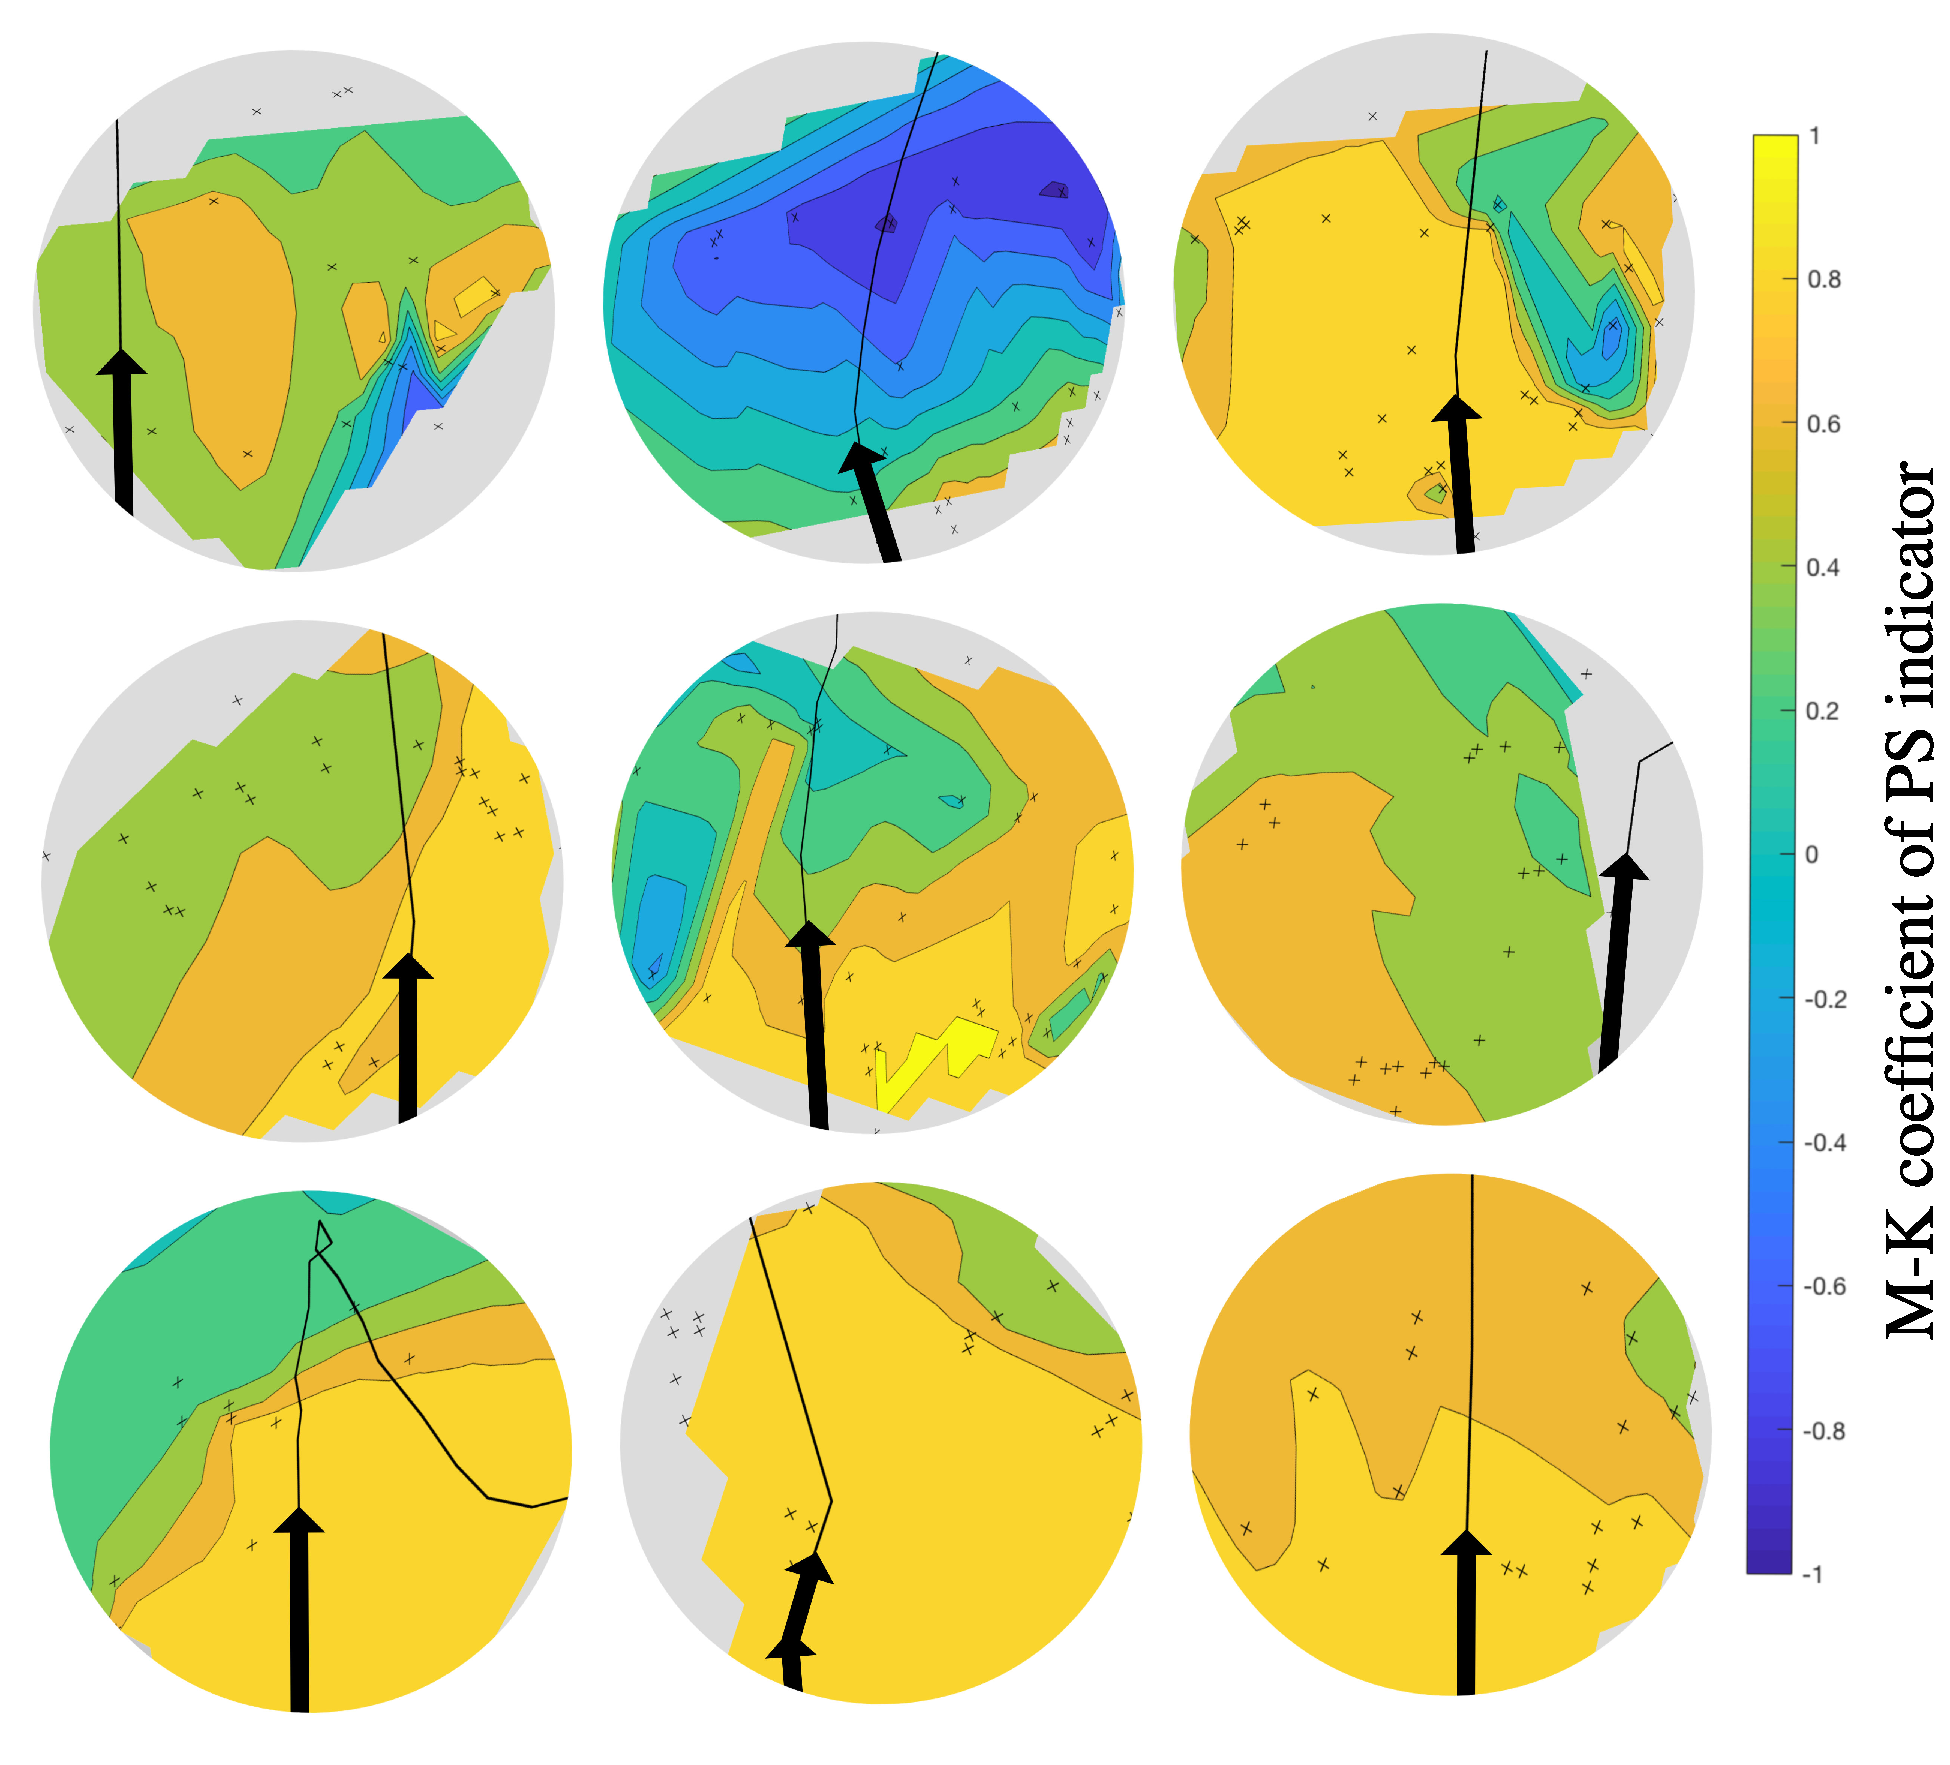
\includegraphics[width = 0.9\textwidth]{Contour3x3}
	\caption{Contour plots of PS indicator gradient for nine Atlantic hurricanes on the Caribbean and Florida coastlines of the USA. left to right: Andrew (Florida); Andrew (Louisiana); Katrina; Wilma; Gustav; Matthew; Harvey; Irma; Nate. In each case, the slope of the PS indicator is evaluated using the Mann-Kendall coefficient and the value of this coefficient is plotted over the geographic area. Each plot has been rotated so that the hurricane track is moving from the bottom to the top of the image (shown by the black line, direction indicated by thick black arrow). The locations of the weather stations are shown by crosses; the grey areas fall outside of the polygon enclosing the weather stations and are therefore not interpolated onto.}
	\label{fig_ContourMapSummary} 
\end{figure}

The value of the Mann-Kendall coefficient of the PS indicator is plotted as a filled contour plot over the geographic area. In figure~\ref{fig_ContourMapSummary} we present a summary of the results: in each case, the contour map is rotated so that the forward path of the Hurricane is moving from the bottom to the top of the image. Hurricane tracks, obtained from the NOAA HURDAT2 dataset (see section~\ref{subsec:TC:data:HURDAT}) are shown by the black line. We are generally able to see a movement of the hurricane from areas with a high value of the Mann-Kendall coefficient, towards areas with lower value, as we expect. Whilst this doesn't provide a useful EWS, it is clear that the PS indicator provides a more robust EWS when applied to many time series in a region than when applied to individual series, as in figure~\ref{fig:TC:1DindicatorsSLP}d.






\section[A tropical cyclone model]{A model of sea-level pressure in tropical cyclones}
\label{sec:TC:Model}

{\Red{
In this section we develop a model of the pressure profile of an approaching tropical cyclone, based on the simple deterministic model developed by \cite{holland1980}. We aim to add a stochastic component to the model which we will parametrise using the early warning signals from the PS and ACF1 indicators obtained in section~\ref{sec:TC:1Dtechniques}. It is expected that by using the values of the PS and ACF1 indicators, obtained from our study of actual sea-level pressure data, we will be able to recreate the stochastic component of the sea-level pressure as observed in the actual data and, by adding this into the model, obtain something that looks like a genuine sea level pressure signal. If we are able to parametrise our stochastic model in this way it will be a verification of effectiveness of the PS indicator in obtaining useful information about the system. {\Red{This model has been presented in \cite{prettyman2019}.}}

We emphasise that it is with this goal of verifying the effectiveness of our techniques in mind that we proceed to develop the model of a tropical cyclone including a stochastic component. It is not with a view towards using the model for practical modelling or forecasting purposes, although this may be interesting subject for future work to be achieved by further developing the model presented here.
}}

\subsubsection{The deterministic model}

\citet{holland1980} presents a simple analytic model of the pressure profile $p$ of a hurricane:
	\begin{equation}
		p(r) = p_c + (p_n-p_c)\exp\left( \frac{-A}{r^B} \right),
	\label{eqn:TC:hollandmodel}
	\end{equation} 
where $r$ is the radial distance from the centre of the hurricane, $p_c$ and $p_n$ are the central and ambient pressures, $A$ and $B$ are parameters to be determined by fitting to observed data. \cite{holland1980} fits the model to three Australian hurricanes: Tracy (December 1974), Joan (December 1975) and Kerry (February 1979). The values of parameters $A$ and $B$ are obtained by fitting to sparse observations, particularly the observations of maximum wind speed $V_m$ given by
	\begin{equation}
		V_m = \left(\frac{B(p_n-p_c)}{\rho e}\right)^{1/2}\,,
		\label{eqn:TC:model:V_m}
	\end{equation} 
and occurring at a radius $R_w = A^{1/B}$. 

Here we present a similar model modified so that the pressure is modelled at a fixed point in space as a function of time, rather than a profile modelled at a fixed time as a function of the distance from the hurricane centre. We are therefore able to model the effect on sea level pressure (at a weather station, for example) of an approaching hurricane. 
We use the values $A=40$ and $B=1$ which are obtained by fitting to Hurricane Katrina (2005) at peak intensity. We consider a fixed point at distance~$d(t)$ from the hurricane centre at time~$t$. In equation~\ref{eqn:TC:hollandmodel}, we replace $r$ by $d(t)$ to introduce a time dependence. We assume the hurricane moves in a straight line towards the fixed point with a speed of $v(t)$~kmph, in which case we have $d(t) = \int_0^t v(s) ds$. For this model, a constant velocity will suffice: 18~kmph is obtained by taking a mean of the nine tropical cyclones studied in section~\ref{sec:TC:field_data} using the HURDAT2 data (see section~\ref{subsec:TC:data:HURDAT}). We in fact use a constant velocity sampled uniformly from the range~$[16,20]$ so that not all implementations of the model are identical. The ambient pressure, $p_n$, is given by 
	\begin{equation}
		p_n(t) = 1016 + 5\eta_1 + 1.6\sin\left(\frac{2\pi t}{12} + K\right),
	\label{eqn:TC:ambientpressure}
	\end{equation} 
where the sine wave models the 12-hourly tidal oscillations and $K$ is a random offset chosen uniformly in the range {\Red{$[0,2\pi]$}}. The central pressure is given by $p_c = 950+10\eta_2$. Values $\eta_1$ and $\eta_2$ are sampled from a standard normal distribution. The reason for the inclusion of $\eta_1$, $\eta_2$ and the random offset $K$ is that we may wish to run the model multiple times and take the mean of statistics over those simulations to obtain an ensemble estimate. For this purpose, we would not want all of the sine wave components to be aligned, nor for all the models to have exactly the same initial parameters.

\subsubsection{The stochastic component}

{\Red{
We observe, in the HURDAT2 sea-level pressure data, that fast-scale noisy fluctuations occur in the times series on top of the large-scale dynamics and the 12-hour tidal oscillations. These fast-scale fluctuations are not included in equation~\ref{eqn:TC:hollandmodel}, but we wish to model them as an additional stochastic component. 
}}

There is also a need to model the increasing memory in the pressure signal, shown to exist using the PS indicator. We therefore add a noise signal to the output in which the power spectrum scaling exponent $\alpha$ increases over time. The maximum value of $\alpha$ is greater for points closer to the cyclone track, and the time at which the maximum value is reached is the time at which the closest approach occurs, which we call $T_{\min}$. We have used values such that $\alpha=0.4$ for $t<t_{\min}-50$ (more than fifty hours before the minimum approach distance is reached). In the 50-hour window, the value of $\alpha$ increases linearly from the background value of $0.4$ to a higher value $\alpha_0$. $\alpha_0$ takes the value 2 in cases where the hurricane path passes directly over the grid-point in question (an approach distance of zero) and decreases linearly with increasing distance from the cyclone track, to a minimum value of $0.4$ for grid-points more than 200km distant.

The part of the noise signal with increasing $\alpha$ value is made by concatenating 10 sub-series, each of length 1000 and with a higher $\alpha$ value than the last (covering the range $[0.4, \alpha_0]$), then sampling with an interval size chosen to give a series of the desired length. All of the noise signals in the model are generated by the method detailed by \citet{kasdin1995}.

We therefore have the model:
	\begin{equation}
		p(d(t)) = p_c + (p_n(t)-p_c)\exp\left( \frac{-A}{d(t)^B} \right) + \eta_t,
	\label{eqn:TC:OurOwnModel}
	\end{equation} 
where $d(t)$ is the distance to the centre of the hurricane at time $t$, $p_c$ is the central pressure, $p_n(t)$ is the ambient pressure at time $t$ given by equation \ref{eqn:TC:ambientpressure}, $A=40$ and $B=1$ are fitted parameters, and $\eta_t$ is a noise term with changing power spectrum scaling exponent as described above. For every point on a spatial grid we are able to calculate the distance $d(t)$ using simple geometry (we model the hurricane as moving in a straight line for simplicity), generate the noise series $\eta$ and then calculate the pressure at that point using equation \ref{eqn:TC:OurOwnModel}. 

We model sea-level pressure at a single point in space which is approached by a hurricane passing by at a distance of 20km, the model uses a time-step of 0.05 hours and 100 implementations are evaluated. We then calculate the ACF1 and PS indicators in a 100-hour sliding window in order to compare them with the results in figure~\ref{fig:TC:1DindicatorsSLP}. The result is shown in figure~\ref{fig_model100}. We see that the ACF1 and PS indicators behave similarly to the result from the real sea-level pressure data, and the pressure series itself also looks reasonable. 

\begin{figure}
	\centering
	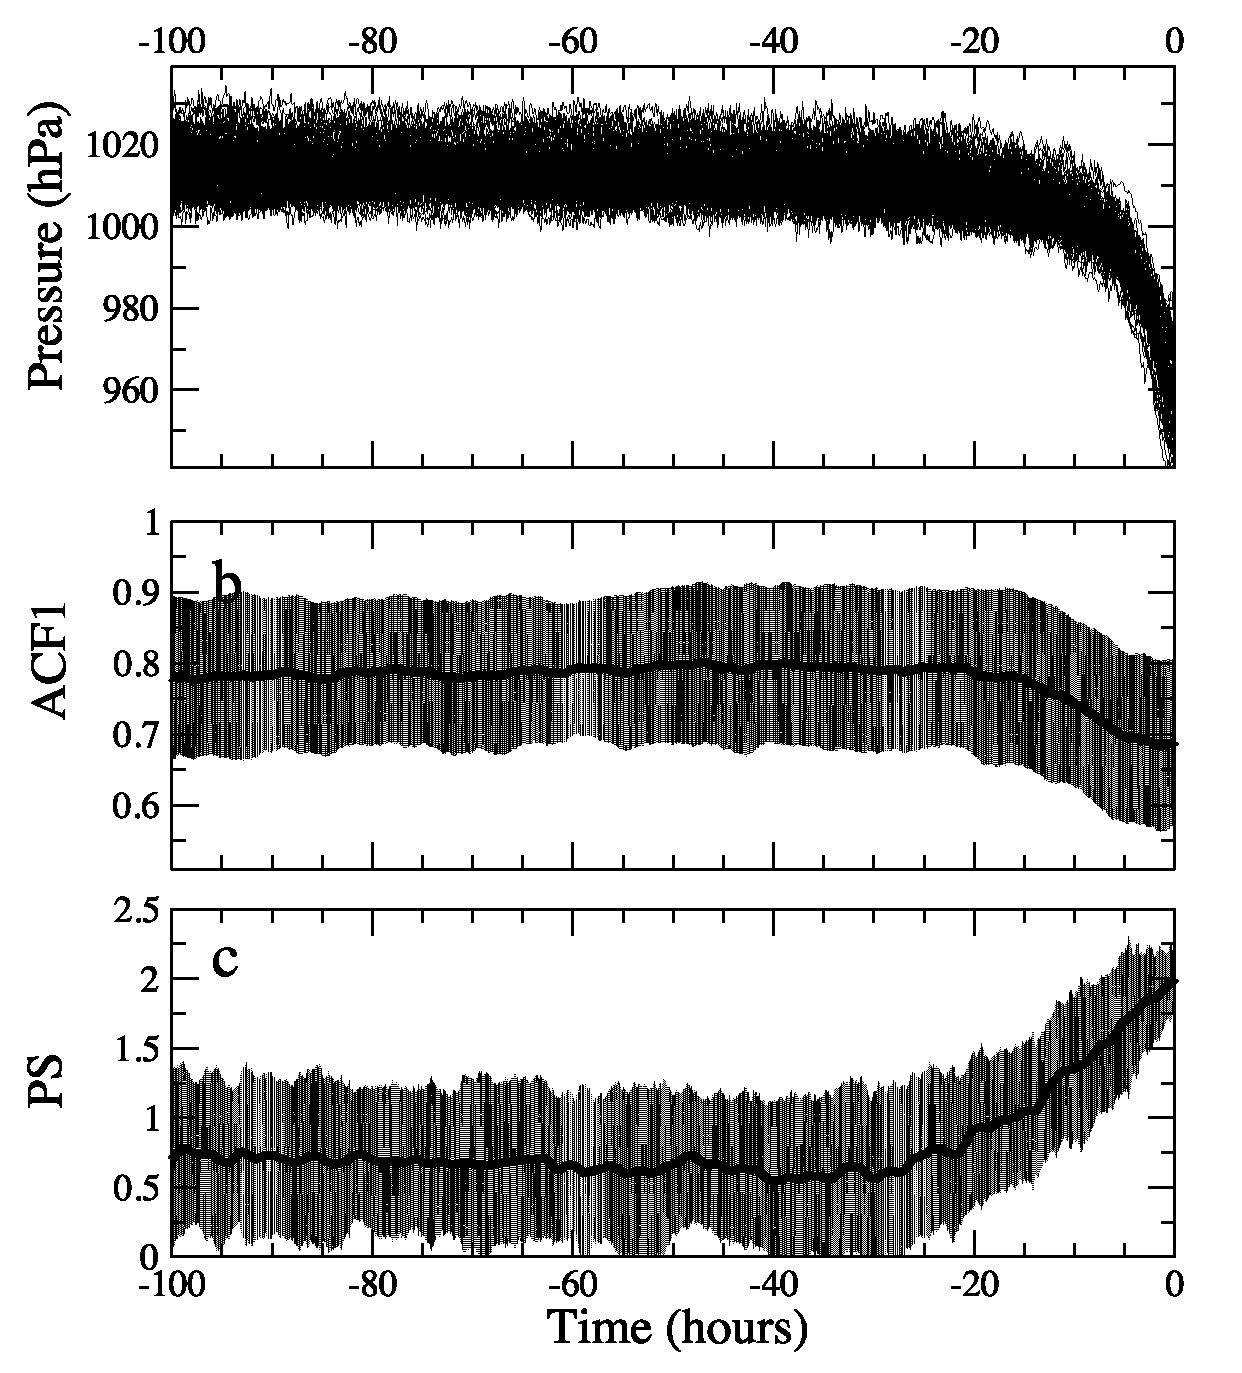
\includegraphics[width = 0.9\columnwidth]{simpleModel100}\caption{\label{fig_model100} Model data (see equation~\ref{eqn:TC:OurOwnModel}) and its EWS indicators. Top panel: 100 instances of the tropical cyclone model. Middle panel: the mean ACF1 indicator. Bottom panel: the mean PS indicator, shown with error bars of one standard deviation.}
\end{figure}

The model is then evaluated with a time-step of 0.05 hours at 100 points in a ten-by-ten grid with 40km spatial separation between points (giving a square of side 360km). The hurricane is modelled as travelling from ‘south' to ‘north' from 400 hours before reaching the bottom of the grid up to the point where it reaches the top of grid. The PS indicator of the pressure signal for each grid-point is calculated in a 100-hour sliding window (of 20,000 points). We then calculate the PS indicator slope, evaluated using the Mann-Kendall coefficient, in the exact same way as shown in the previous section (figure~\ref{fig_ContourMapSummary}), in the 30-hour window before the hurricane reaches the bottom of the grid. Figure~\ref{fig_tenModelRuns} shows the mean over ten such evaluations for ten separate runs of the model. We see that the pattern is consistent with our expectations and also with the general pattern of the analysis of real data in figure~\ref{fig_ContourMapSummary}. This confirms our understanding of the hurricane statistics.

\begin{figure}
	\centering
	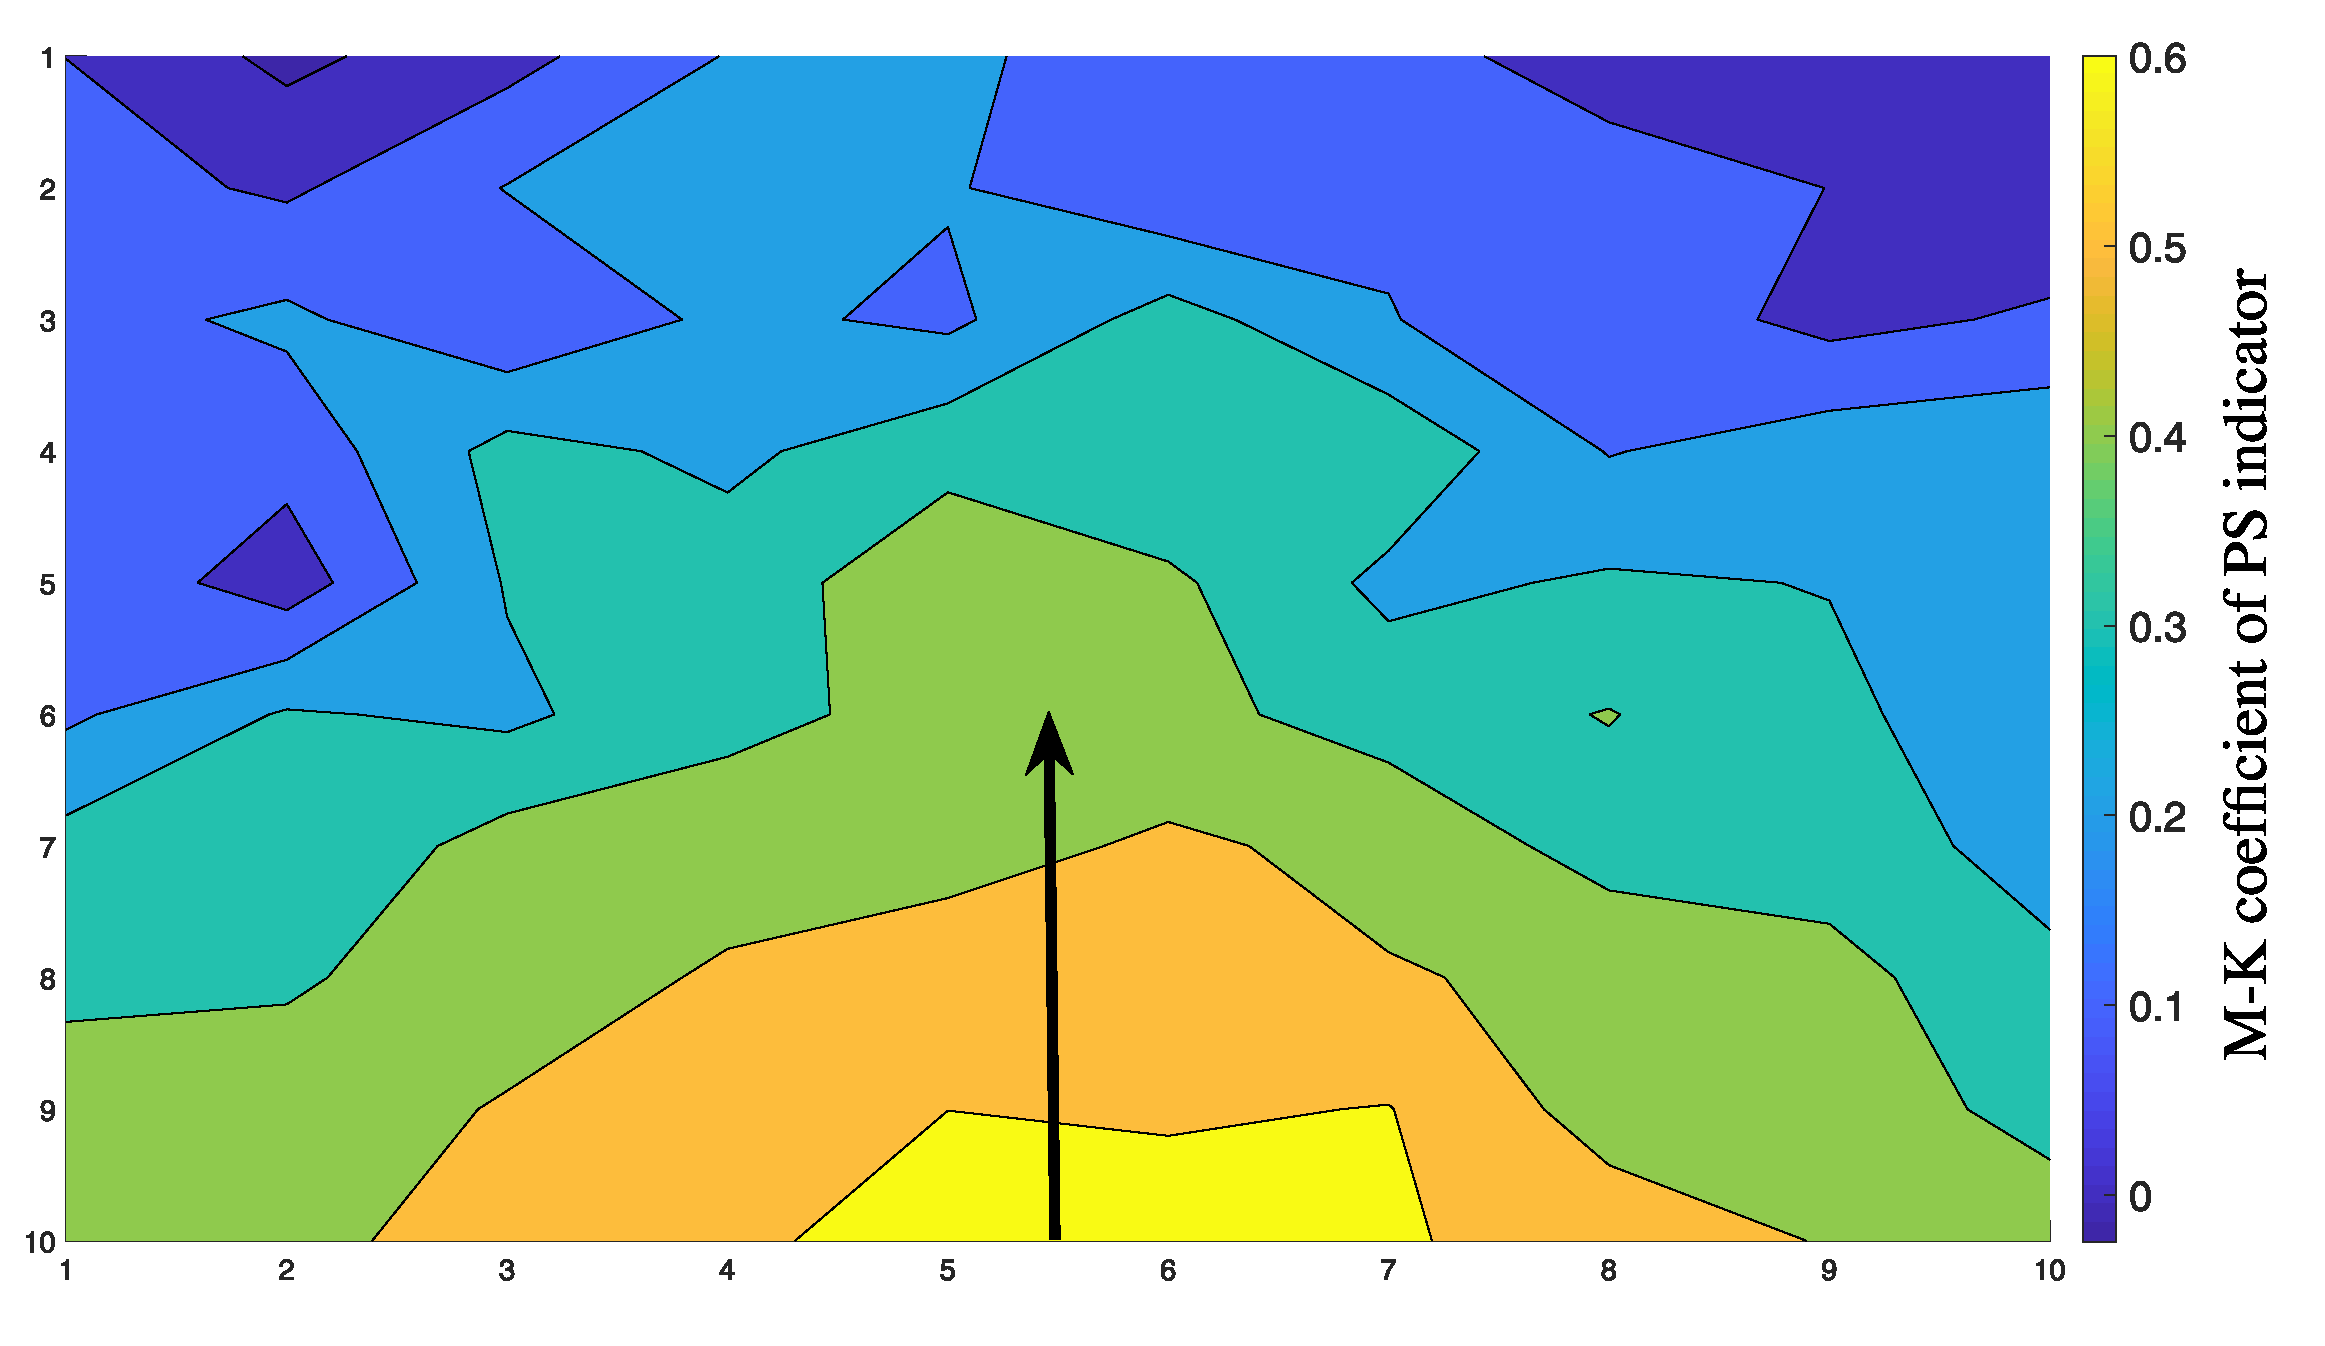
\includegraphics[width = 0.9\textwidth]{07_tenModelRuns}\caption{\label{fig_tenModelRuns} The mean of the PS indicator slope (evaluated using the Mann-Kendall coefficient) over ten realisations of the hurricane model. The slope is evaluated for the PS indicator of the pressure signal at each of 100 grid points with 20km spacing, in a 30-hour window before the modelled hurricane reaches the bottom of the image. The motion of the hurricane is shown by the black arrow.}
\end{figure}


\section{Discussion}\label{sec:TC:discussion}

We have applied the tipping point indicators introduced in chapters~\ref{chap:1D} and~\ref{chap:2D} to the meteorological variables measured in the vicinity on an approaching tropical cyclone. When applied to the sea-level pressure data, the ACF1 and DFA indicators do not appear to provide an EWS. {\Red{\label{pageref:TC:exaggeration} However, looking at the mean over the ensemble of fourteen cases, the PS indicator appears to begin to increase around 48 hours before the lowest pressure, although this increase is not significant when considering the error in the signal. This is about the same point ($-48$ hours) that the decreasing trend in pressure becomes visible, suggesting that it may be able to provide a detectable EWS in this context, if longer time series and larger ensembles were available.}} The methods used to incorporate wind speed data into the analysis besides sea-level pressure have not appeared to yield any improvement, this is possibly due to the two variables being closely correlated. 

We have also attempted to increase the robustness of the results provided by the PS indicator by including data from many points in a close geographical region. This has not produced a reliable early warning signal but it has allowed us to visualise an approaching storm by plotting the strength of the increasing trend in the PS indicator over the region. We have therefore confirmed that in this specific system the PS indicator increases consistently prior to and during the tipping event, which is not a bifurcational tipping, whilst the DFA indicator shows no change (see section~\ref{sec:TC:1Dtechniques}). {\Red{\label{pageref:TC:scaling_comment} This is not unexpected since claims that the DFA and PS scaling exponents are linearly related \citep{heneghan2000} are assuming power-law scaling of the power spectrum and DFA segment sizes, whereas we are estimating the PS exponent even in the absence of power-law scaling, as justified by the analysis in section~\ref{subsec:1D:Exponents_as_EWS:nopowerlawsacaling} (page~\pageref{subsec:1D:Exponents_as_EWS:nopowerlawsacaling}). }}

We note that the tropical cyclone example was chosen because it appears to exhibit tipping behaviour whilst not being described, according to our current knowledge, by a bifurcating or state-switching dynamical system often associated with tipping point analysis, therefore presenting the opportunity to apply known methods in a novel system. In future work it will be interesting to apply the PS indicator in other applications where it may be compared to the existing ACF1 and DFA indicators. In particular, the methods applied in section~\ref{sec:TC:field_data} to sea-level pressure data over a geographic area could usefully be applied to the greening and desertification of the Sahara, similarly to the methods presented by \citet{bathiany2013p1} (discussed in section~\ref{sec:2D:ExtensionToGridded}). At the time of writing, model data with sufficient temporal resolution are not available.  

%%%%%%% Cyclogenesis

%schreck2015kelvin
%graf2017objective
%kilroy2017unified
%riehl1950model
%schecter2009hurricane

%maestre2009patch -- vegetation patches for desertification
%lin2010spatial -- 
%kefi2014early
%dakos2011slowing

Another interesting system worth studying with these methods is the formation, rather than the approach, of a tropical cyclone (cyclogenesis) since this is closer to the idea of a complex system undergoing a critical transition \citep{scheffer2009} and therefore a better candidate for tipping point analysis. However, real-life data, at a resolution suitable for tipping point analysis, is not available to our knowledge: it is unlikely that measurements would be taken at the precise location of cyclogenesis. Moreover, there are many different conditions under which cyclogenesis occurs \citep{graf2017objective, kilroy2017unified} and many influencing external factors \citep{schreck2015kelvin}. Since the original aim of this study was to investigate the behaviour of tipping point indicators in a novel system, not necessarily to produce a result useful to practical prediction problems, it was not necessary to select a system with typical bifurcational tipping point dynamics. Rather, the availability of data was the primary concern. A future project, however, could apply tipping point indicators to data from cyclogenesis models, such as the model presented in \citet{schecter2009hurricane} which shows an ordered hurricane forming from a turbulent initial state, producing an image resembling models of tipping points in vegetation coverage \citep{dakos2011slowing, kefi2014early} in which early warning signals have been detected.

We have also presented a simple model of an approaching tropical cyclone parametrised using observed trends in tipping point indicators. {\Red{We suggest that the nature of the noise present in this model is similar to the noise found in a real sea-level pressure signal since we have used our analyses of real sea level pressure time series in the vicinities of tropical cyclones to parametrise the stochastic component of the model. }}